% Options for packages loaded elsewhere
\PassOptionsToPackage{unicode}{hyperref}
\PassOptionsToPackage{hyphens}{url}
%
\documentclass[
]{book}
\usepackage{amsmath,amssymb}
\usepackage{lmodern}
\usepackage{ifxetex,ifluatex}
\ifnum 0\ifxetex 1\fi\ifluatex 1\fi=0 % if pdftex
  \usepackage[T1]{fontenc}
  \usepackage[utf8]{inputenc}
  \usepackage{textcomp} % provide euro and other symbols
\else % if luatex or xetex
  \usepackage{unicode-math}
  \defaultfontfeatures{Scale=MatchLowercase}
  \defaultfontfeatures[\rmfamily]{Ligatures=TeX,Scale=1}
\fi
% Use upquote if available, for straight quotes in verbatim environments
\IfFileExists{upquote.sty}{\usepackage{upquote}}{}
\IfFileExists{microtype.sty}{% use microtype if available
  \usepackage[]{microtype}
  \UseMicrotypeSet[protrusion]{basicmath} % disable protrusion for tt fonts
}{}
\makeatletter
\@ifundefined{KOMAClassName}{% if non-KOMA class
  \IfFileExists{parskip.sty}{%
    \usepackage{parskip}
  }{% else
    \setlength{\parindent}{0pt}
    \setlength{\parskip}{6pt plus 2pt minus 1pt}}
}{% if KOMA class
  \KOMAoptions{parskip=half}}
\makeatother
\usepackage{xcolor}
\IfFileExists{xurl.sty}{\usepackage{xurl}}{} % add URL line breaks if available
\IfFileExists{bookmark.sty}{\usepackage{bookmark}}{\usepackage{hyperref}}
\hypersetup{
  pdftitle={Estudo da Bíblia},
  pdfauthor={José Roberto Costa Moretti},
  hidelinks,
  pdfcreator={LaTeX via pandoc}}
\urlstyle{same} % disable monospaced font for URLs
\usepackage{longtable,booktabs,array}
\usepackage{calc} % for calculating minipage widths
% Correct order of tables after \paragraph or \subparagraph
\usepackage{etoolbox}
\makeatletter
\patchcmd\longtable{\par}{\if@noskipsec\mbox{}\fi\par}{}{}
\makeatother
% Allow footnotes in longtable head/foot
\IfFileExists{footnotehyper.sty}{\usepackage{footnotehyper}}{\usepackage{footnote}}
\makesavenoteenv{longtable}
\usepackage{graphicx}
\makeatletter
\def\maxwidth{\ifdim\Gin@nat@width>\linewidth\linewidth\else\Gin@nat@width\fi}
\def\maxheight{\ifdim\Gin@nat@height>\textheight\textheight\else\Gin@nat@height\fi}
\makeatother
% Scale images if necessary, so that they will not overflow the page
% margins by default, and it is still possible to overwrite the defaults
% using explicit options in \includegraphics[width, height, ...]{}
\setkeys{Gin}{width=\maxwidth,height=\maxheight,keepaspectratio}
% Set default figure placement to htbp
\makeatletter
\def\fps@figure{htbp}
\makeatother
\setlength{\emergencystretch}{3em} % prevent overfull lines
\providecommand{\tightlist}{%
  \setlength{\itemsep}{0pt}\setlength{\parskip}{0pt}}
\setcounter{secnumdepth}{5}
\usepackage{booktabs}
\usepackage{amsthm}
\makeatletter
\def\thm@space@setup{%
  \thm@preskip=8pt plus 2pt minus 4pt
  \thm@postskip=\thm@preskip
}
\makeatother
\ifluatex
  \usepackage{selnolig}  % disable illegal ligatures
\fi
\usepackage[]{natbib}
\bibliographystyle{apalike}

\title{Estudo da Bíblia}
\author{José Roberto Costa Moretti}
\date{Texto finalizado 29 de agosto de 2020}

\begin{document}
\maketitle

{
\setcounter{tocdepth}{1}
\tableofcontents
}
\hypertarget{capa}{%
\chapter*{Capa}\label{capa}}
\addcontentsline{toc}{chapter}{Capa}

\begin{center}\includegraphics[width=0.7\linewidth]{Estudo da Bíblia} \end{center}

\hypertarget{prefuxe1cio}{%
\chapter*{Prefácio}\label{prefuxe1cio}}
\addcontentsline{toc}{chapter}{Prefácio}

Na manhã do dia que meu pai foi internado, de onde 15 dias mais tarde iria partir ao encontro de Deus e Nossa Senhora, recebi dele por e-mail a versão final deste texto. Naquele momento não compreendi o que estava por acontecer. No entanto, em poucos dias entendi que além de estar se despedindo e desejando que eu e minha família fossemos felizes, meu pai também pedia indiretamente naquela mensagem que eu divulgasse este estudo. Ele sempre me dizia que o texto que ele estava redigindo poderia ajudar as pessoas a compreender melhor a Palavra de Deus e alcançar a Salvação.

Este Estudo da Bíblia resultou de um esforço de 2 anos realizado por meu pai. Nos momentos em que estive com ele neste período, me recordo dele sempre ter dedicado parte do seu dia sublinhando trechos da sua Bíblia e redigindo este texto no computador. Meu pai continuou firme no seu objetivo, mesmo nos seus últimos meses vida, quando sua enfermidade havia se agravado significativamente.

Após alguns meses do seu falecimento, consegui fazer a leitura deste texto e decidi que eu mesmo iria estruturá-lo na forma de um livro digital que pudesse ser rapidamente divulgado e facilmente acessado. Em uma linguagem simples e clara, este estudo reforça as passagens e lições mais importantes da Bíblia, servindo tanto de apoio para os que já possuem o hábito de ler a Palavra de Deus quanto de estímulo para aqueles que ainda não possuem este hábito.

Desejo uma boa leitura a todos e peço que sempre que passarem em frente a Igreja de Lourdes, na Rua da Bahia em Belo Horizonte, rezem pela alma do meu pai. Ali, junto de Nossa Senhora, estão depositadas as cinzas de um homem que foi um exemplo de fé.

\emph{Marcelo S. Moretti}

\begin{center}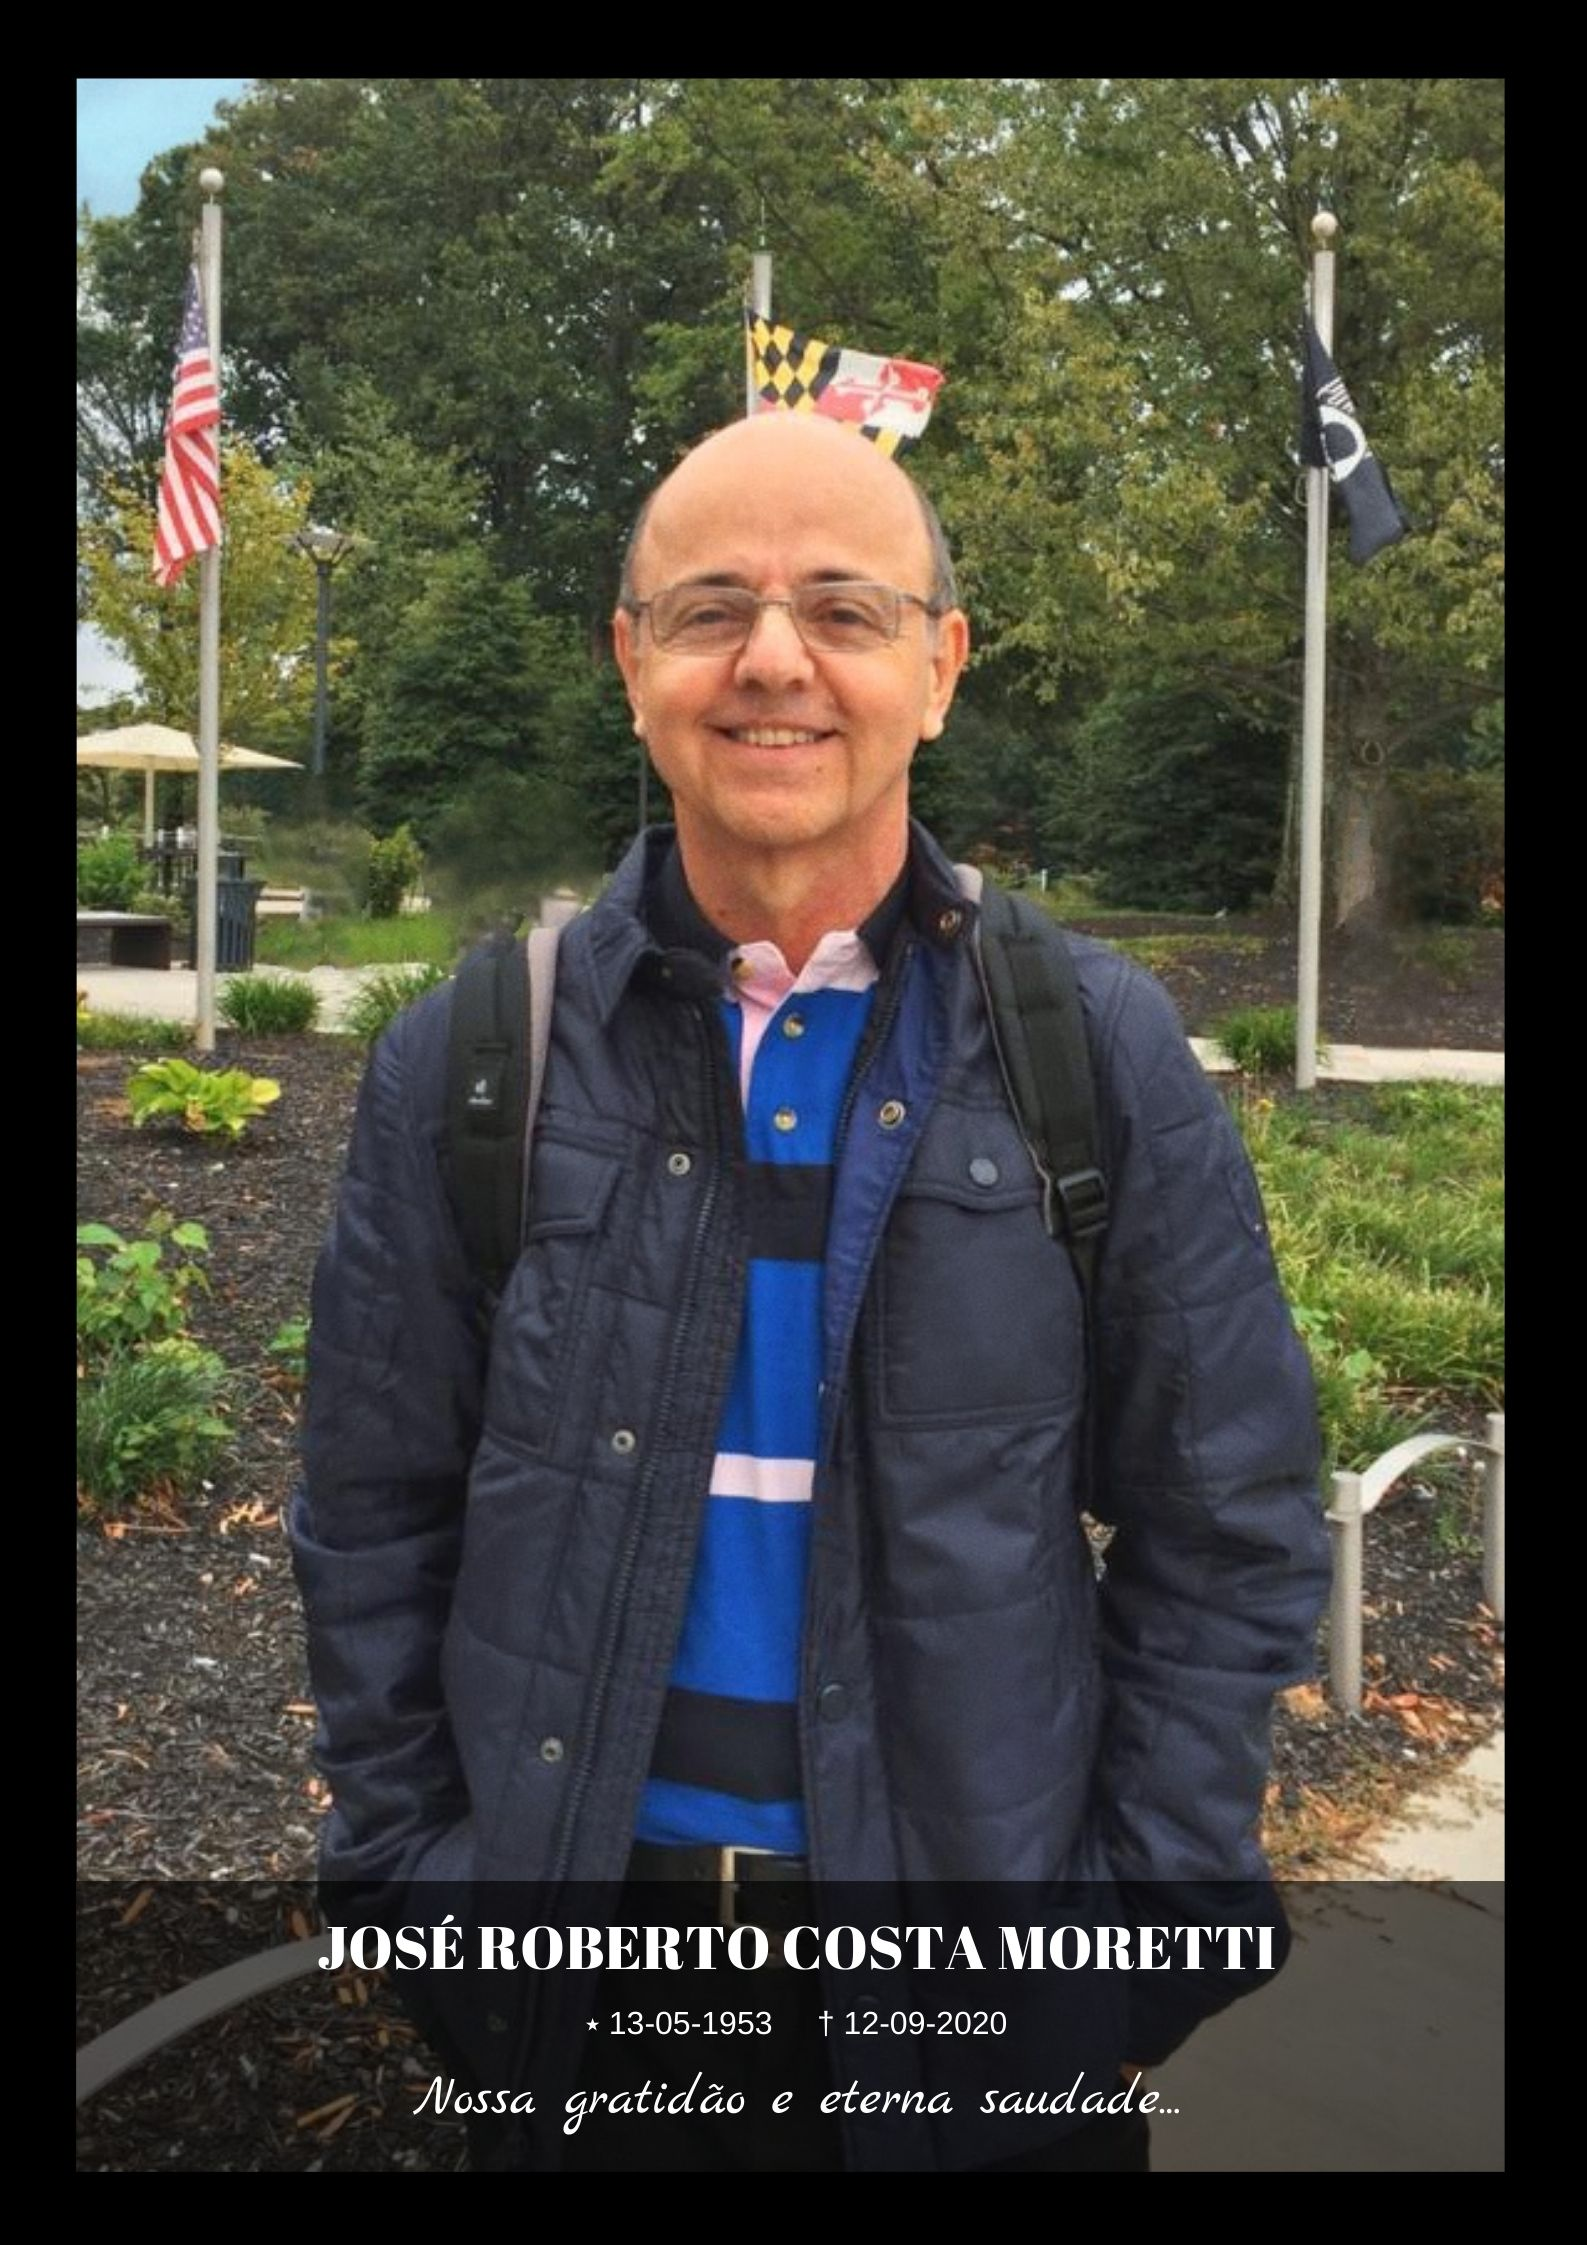
\includegraphics[width=0.7\linewidth]{Lembrança Moretti} \end{center}

\hypertarget{parte-i-explicando-o-antigo-testamento}{%
\chapter*{Parte I: Explicando o Antigo Testamento}\label{parte-i-explicando-o-antigo-testamento}}
\addcontentsline{toc}{chapter}{Parte I: Explicando o Antigo Testamento}

\hypertarget{pentateuco}{%
\section*{1. Pentateuco}\label{pentateuco}}
\addcontentsline{toc}{section}{1. Pentateuco}

Conjunto de cinco livros: Genesis (origem), Êxodo (Saída e Libertação), Levítico (Leis), Números (Recenciamento) e Deuteronômio (Segunda Lei). Na Bíblia hebraica (\textbf{Tanah}) os judeus referem-se a esses livros como \textbf{Torá} -- Lei.

\hypertarget{genesis}{%
\section*{2. Genesis}\label{genesis}}
\addcontentsline{toc}{section}{2. Genesis}

O primeiro livro da Bíblia porque nele encontramos as narrativas sobre as origens do mundo, da humanidade, do pecado e da história do povo de Deus a partir de Abraão. Ao que tudo indica ele foi escrito durante o exilio da Babilônia entre os anos 586 a 538 AC.

\hypertarget{pecado-de-aduxe3o-e-eva}{%
\section*{3. Pecado de Adão e Eva}\label{pecado-de-aduxe3o-e-eva}}
\addcontentsline{toc}{section}{3. Pecado de Adão e Eva}

Pecado da autossuficiência, do orgulho de desejarem ser como Deus, para poder dominar e explorar o seu semelhante. Adão e Eva desejaram o conhecimento do bem e do mal segundo critérios próprios, deixando de lado a sabedoria e a Lei de Deus (Gn 1, 28; 2, 16; 2,17; 3, 35).

\hypertarget{fruto}{%
\section*{4. Fruto}\label{fruto}}
\addcontentsline{toc}{section}{4. Fruto}

O fruto simboliza a eterna tentação do homem em não querer conhecer-se diante de Deus, mas querer comportar-se por si mesmo, escolher o próprio caminho. Comer do fruto (maça) é deixar Deus e seguir a si próprio.

\hypertarget{serpente}{%
\section*{5. Serpente}\label{serpente}}
\addcontentsline{toc}{section}{5. Serpente}

Significa a tentação, aquela inclinação que todos nós temos para o mal.

\hypertarget{torre-de-babel}{%
\section*{6. Torre de Babel}\label{torre-de-babel}}
\addcontentsline{toc}{section}{6. Torre de Babel}

A narrativa explica a causa de tantas línguas existentes no mundo. Segundo o autor, a causa é fruto do orgulho do homem, o que faz que a humanidade perca a unidade. Babel significa confusão.

\hypertarget{manuxe1}{%
\section*{7. Maná}\label{manuxe1}}
\addcontentsline{toc}{section}{7. Maná}

O maná era semelhante a semente do coentro e tinha aparência de resina. O povo se espalhava para juntá-lo e esmagava no moinho ou moía no pilão; depois cozinhava numa panela e fazia pão e bolos.

\hypertarget{uxeaxodo}{%
\section*{8. Êxodo}\label{uxeaxodo}}
\addcontentsline{toc}{section}{8. Êxodo}

Sabemos que o povo de Deus (Israel), devido a uma grande fome, veio para o Egito quando José era vice-governador. Os hebreus da época (1500 AC) perceberam que estavam sendo explorados e escravizados. Deus ouve suas preces e envia Moisés como instrumento de libertação, o que aconteceu por volta de 1250 AC. A palavra êxodo significa saída. O livro descreve a saída da escravidão do Egito, a passagem pelo Mar Vermelho e também os dez Mandamentos dados por Deus através de Moisés no Monte Sinai. Descreve a caminhada do povo ao longo de 40 anos pelo deserto. Com isso o povo está caminhando com a proteção de Deus rumo à liberdade e à Terra Prometida.

\hypertarget{levuxedtico-leis}{%
\section*{9. Levítico (Leis)}\label{levuxedtico-leis}}
\addcontentsline{toc}{section}{9. Levítico (Leis)}

Levítico provém do nome de Levi, a tribo de Israel que foi escolhida para exercer a função sacerdotal no meio do povo. O livro fala de sacrifícios, holocaustos (sacrifício no qual a vítima é queimada completamente) e oblações (oferecimento de alimentos, as primícias, ou seja, os primeiros frutos). Relata também a Lei do puro e do impuro: lei terrível que causou tantos sofrimentos no povo do Antigo Testamento, de modo mais intenso após Esdras e Neemias (pós-exílio da Babilônia). Puro era a pessoa sem pecado e que tinha condições de participar do culto e estar próxima de Deus. Impuro era a pessoa que devia ser excluída de participar do culto a Deus (tem mais sentido num ato físico do que condição moral). Para ser impuro bastava ingerir alguns alimentos, como por exemplo, carne de porco, ter lepra, tocar em mortos e em algumas atividades sexuais. Até Jesus critica esta lei: Não é o que entra na boca que torna o homem impuro, mas o que sai da boca. Pois é do coração que vem as más intenções, crimes, adultério, imoralidade, roubos, falsos testemunhas e calunias (Mt 15, 11, 19-20).

\hypertarget{nuxfameros}{%
\section*{10. Números}\label{nuxfameros}}
\addcontentsline{toc}{section}{10. Números}

O livro tem esse nome porque começa com um grande recenciamento do povo ou para descrever o período de 40 anos no deserto. O deserto foi como que um tempo necessário de sofrimentos, lutas, conflitos e de confiança em Deus que caminha com seu povo, a fim de construir uma nova sociedade de justiça e solidariedade. Javé tinha dito que em relação a primeira geração: \emph{Morrerão todos no deserto e não ficará nenhum, além de Caleb, filho de Jefoné, e Josué, filho de Num} (Nn 26,25). Um povo novo e vida nova na Terra prometida. Um texto curioso cita as serpentes venenosas no deserto que picavam e muitos morriam. Javé pediu a Moisés: \emph{Faça uma serpente venenosa e coloque-a sobre um poste. Quem for mordido e olhar para ela ficará curado} (Nn 21,8). Jesus se refere a este texto: \emph{Assim como Moisés levantou a serpente no deserto, do mesmo modo é preciso que o Filho do Homem seja levantado. Assim todo aquele que nesse acreditar, nele terá vida eterna} (Jo 3, 14,-15). Outra citação é a \textbf{benção litúrgica aos filhos de Israel}: \emph{O Senhor disse a Moisés: Dize a Arão e seus filhos: Eis como abençoarei os filhos de Israel: O Senhor te abençoe e te guarde. O Senhor de mostre a sua face e conceda-te sua graça. O Senhor volta o seu rosto para ti e te dê a paz. E assim invocação o meu nome sobre os filhos de Israel e eu os abençoarei} (Nm 6, 22-27).

\hypertarget{segunda-lei-deuteronuxf4mio}{%
\section*{11. Segunda Lei Deuteronômio}\label{segunda-lei-deuteronuxf4mio}}
\addcontentsline{toc}{section}{11. Segunda Lei Deuteronômio}

O texto gira em torno da aliança entre Israel e Deus, ou seja, a fidelidade do povo em relação aos preceitos (Leis) divinos. Lá encontramos a famosa profissão de fé ou oração que os judeus fazem até hoje: O \textbf{``Shemá''} (escutar e ouvir): \emph{Escuta Israel. O Senhor nosso Deus, é o Senhor que é um. Amaras o Senhor, teu Deus, com todo o teu coração, com todo o teu ser, com todas as tuas forças. As palavras dos mandamentos que hoje te dou estarão presentes no teu coração; tu os repetiras a teus filhos. Tu lhes falarás deles quando estiveres em casa e quando andares pela estrada, quando estiveres deitado e quando estiveres de pé} (Dt 6, 4-7).

\hypertarget{mudanuxe7a-de-vida-liberdade-e-conversuxe3o}{%
\section*{12. Mudança de vida (Liberdade e conversão)}\label{mudanuxe7a-de-vida-liberdade-e-conversuxe3o}}
\addcontentsline{toc}{section}{12. Mudança de vida (Liberdade e conversão)}

\emph{Hoje estou colocando diante de você a vida e a felicidade, a morte e a desgraça. Se obedeceres aos mandamentos de Javé seu Deus você viverá e se multiplicará. Todavia, se o seu coração se desviar e você não obedecer perecerão. Hoje eu lhe propus a vida ou a morte, a benção ou a maldição. Escolha, portanto, a vida} (Dt 30, 15-20).

\hypertarget{livros-histuxf3ricos}{%
\section*{13. Livros Históricos}\label{livros-histuxf3ricos}}
\addcontentsline{toc}{section}{13. Livros Históricos}

Narram a história do povo de Deus, desde a entrada na Terra Prometida (Josué) até quase a época de Jesus (Macabeus) por ocasião do domínio grego. \emph{Fica claro que a história de Israel depende da atitude que o povo toma em relação à aliança com Deus. Se o povo é fiel a aliança, Deus concede a benção que traduz no dom da terra e na prosperidade. Se o povo é infiel, atrai para si mesmo a maldição que se concretiza com fracasso e perda da terra, que no Antigo Testamento é igual a vida}. Estes livros estão divididos em 3 grupos:

\begin{itemize}
\item
  Josué, Juízes, 1 e 2 Samuel, 1 e 2 Reis: \emph{Reafirmam que a história de Israel depende da atitude que o povo toma na aliança com Deus}. Se o povo é fiel Deus lhe concede a benção que se traduz no dom da terra e prosperidade.
\item
  1 e 2 Crônicas, Esdras e Neemias, 1 e 2 Macabeus: \emph{Procuram dar as normas básicas para a sobrevivência e organização do povo de Deus depois do exílio da Babilônia e da reconstrução do Templo em Jerusalém e a resistência dos Macabeus contra a dominação grega}.
\item
  Rute, Tobias, Judite e Ester: Estes livros se apresentam como modelos de vivências da fé diante das dificuldades da vida, percebendo claramente a proteção de Deus.
\end{itemize}

\textbf{Josué:} Narra os fatos ocorridos entre 1230 a 1200 AC. O centro deste livro é a questão da posse da terra, vista na Bíblia como fonte de vida, e ao mesmo tempo, como dom de Deus. A terra pertente a Deus e é sagrada por produzir alimentos, gerar vida e ser local de moradia. Não foi pela força ou inteligência humana, muito menos pelo poder das armas que Israel conquista a Terra Prometida e sim, pela atuação direta de Deus em favor dos israelitas. O Povo de Israel deveria ter um novo sistema de ser e agir nesta nova terra: \emph{Nada de opressão, acúmulos, riquezas exorbitantes, escravizações, seria um sistema tribal, onde ninguém era dono da terra e sim Deus. O povo deveria partilhar a terra e seus bens produtivos, lutar pela justiça, igualdade e fraternidade}.

\textbf{Juízes:} O livro recebeu este nome devido aos líderes responsáveis pela sociedade dos hebreus (israelitas) chamados de Juízes. Os acontecimentos compreendem da posse da Terra Prometida (Canaã -- 1200 a 1020 AC), no período chamado de sistema tribal, até quando Israel optou pela monarquia. Os juízes eram encarregados pela política, economia, guerras e lutavam pela justiça e fidelidade a Javé. Dentre eles destacamos: \emph{Débora e Jael, Sansão, Jefté, Gedeão, Samuel e outros}. As constantes guerras e o perigo da idolatria, ou seja, de adoração a outros deuses, principalmente a Baal, o deus cananeu da fertilidade, além dos costumes da ``prostituição sagrada'' (ritual que consiste em relações sexuais realizadas no contexto de um culto religioso) e de muitos outros fatores, fez com que Javé suscitasse vários juízes e juízas. Numa visão ampla, pode-se dizer que a geração revolucionária que conquistou duramente a terra, tinha morrido. Surge uma nova geração e começa o pecado (adoração a Baal), depois vem o castigo (Javé entrega seu povo ao poder de assaltantes de tal forma que os israelitas já não conseguiam resistir), a conversão (os madianitas reduziram Israel à miséria e então eles clamaram a Javé) e a libertação (Javé fez surgir juízes que libertam os israelitas dos assaltantes). Os juízes organizam o povo e o lideram na luta pela libertação. Conta a história de Sansão que salva Israel do poder dos filisteus. Quanto a Jefté ele faz uma promessa imprudente a Javé ao dizer: Se entregares os amonitas em meu poder, então, a primeira pessoa que sair para me receber será oferecida em holocausto. Esta pessoa foi sua única filha. Quanto a juíza Debora e a Jael, que mata Sísara, a história mostra como a força, a coragem e a esperteza femininas são importantes na vida de um povo.

\textbf{Samuel:} A história de Samuel (nome de Deus) descreve a transição entre o sistema tribal para o sistema da monarquia. Ana, sua mãe era estéril. Ela orou e chorou muito diante de Deus e fez um voto: se me deres um filho homem, eu o consagrarei ao Senhor. Elcana conheceu sua mulher Ana e ela concebeu Samuel. Samuel é chamado por Deus 3 vezes. Pensa que é Eli. Somente na quarta vez que ele responde: Fala Javé, pois o teu servo escuta. O livro fala também da Arca da Aliança que era levada a frente dos exércitos quanto saiam para lutar. Samuel alerta a todos do perigo de um sistema de monarquia onde o rei tem autoridade máxima, exige tributos, mão de obra escrava, desapropriação de terras, exército, exploração. Com os juízes o povo não era explorado. O primeiro rei foi Saul que detém todo o poder, guarda para si as riquezas, faz guerras, usa o poder para os próprios interesses e esquece-se dos pobres. Davi, depois da morte de Saul torna-se rei. Davi pecou, pois assassinou Urias, o heteu, para poder casar com a mulher dele. Em 2Sm, 7, 12-16 encontramos \textbf{a profecia de Natã} a respeito da permanência da linhagem davítica sobre o trono de Israel: \emph{A dinastia e a realeza dele permanecerão firmes para sempre diante de mim, e o seu trono será sólido para sempre} (2Sm 7,16).

\textbf{1 e 2 Reis:} A maioria dos reis não foi fiel a Javé. Surgem nesta época os primeiros profetas que anunciam o projeto de Deus e denunciam as injustiças e defendem o povo da exploração dos reis (os primeiros reis: Saul, Davi e Salamão). O livro dos Reis se baseia em competições, lutas, sangue e morte. É a história do poder e da ambição, do poder pelo poder, da ganância e da corrupção fruto da vontade humana e não de Deus. Os livros dos Reis abrangem os acontecimentos que cobrem o período de mais de quatrocentos anos, desde o Rei Salomão (971 AC) até o Rei Jeconias (561 AC). Após a morte de Salomão (931 AC) sobe ao poder seu filho Roboão que deseja servir ao povo. A corte aconselha o contrário: aumentar a exploração para não perder a autoridade. Isto gera um conflito entre Roboão e Jeroboão. Este é proclamado Rei do Norte, cuja capital é Samaria, e Roboão é proclamado rei do Sul, cuja capital é Jerusalém. De todos os reis que governaram Israel somente Davi, Ezequias e Josias são considerados bons. Os demais não combateram a idolatria. O reino do Norte (Israel) caiu em 722 AC: o rei Salmanasar V da Assíria invadiu Israel, após o rei Oseias ter recusado a pagar tributo aos assírios e conquistou Israel). Após a queda do reino do Norte o reino do Sul (Judá) viveu anos de paz e caiu somente em 586 AC quando Jeconias era rei. Nabucodonosor foi rei da Babilônia e conquistou Judá. Está também no livro dos Reis a história do Profeta Elias e de Elizeu: o livro cita as passagens de Elias com a viúva de Sarepta quando não havia mais farinha e azeite. E Elias diz: a vasilha de farinha e a vasilha de azeite não ficaram vazias até o dia em que Javé mandar chuva sobre a terra (1Rz 17,14). Narra também a ressurreição do menino conforme pedido de Elias a Javé (1Rs 17, 17-24). O livro cita também a cura de Naamã pelo profeta Elizeu (sucessor de Elias): Naamã mergulha 7 vezes no rio Jordão e fica curado da lepra (2Rs 5).

\begin{itemize}
\item
  Resumo da vida do profeta Elias: Elias, cujo nome significa ``Jeová é Deus'' foi chamado por Deus para o ministério profético, em um dos piores períodos da história de Israel. \emph{Elias profetizou em um período marcado por crise, fome, miséria, corrupção e apostasia. Mas, em meio à crise moral, social e espiritual}. Deus pôde contar com a coragem e a determinação de Elias, para ser seu porta-voz. \emph{Elias foi profeta do Reino do Norte, nos reinados do Rei Acabe e do seu filho Acazias. Ele desafiou o povo a fazer uma escolha definitiva entre seguir a Deus ou a Baal}. Os israelitas achavam que podiam adorar o Deus verdadeiro e ao mesmo tempo adorar a Baal. \emph{Eles tinham o coração dividido e por esta razão queriam servir a dois senhores}. Jesus, durante o seu ministério terreno advertiu contra essa atitude fatal: \emph{``Ninguém pode servir a dois senhores, porque ou há de odiar um e amar o outro ou se dedicará a um e desprezará o outro''} (Mt 6:24).
\item
  Quem era Elias: O mais famoso e dramático dos profetas de Israel (874 AC). Foi contemporâneo de Acabe, Jezabel, Acazias, Obadias, Jeú e Aazael. \emph{Predisse o início e o fim de uma seca de três anos e meio (IRs 17.1; 18.44). Fugiu da presença de Acabe e foi sustentado pelos corvos e por uma pobre viúva (IRs 17.1-6; 8-16). Foi usado por Deus para ressuscitar uma criança (IRs 17.22). Desafiou os sacerdotes de Baal no Monte Carmelo: dois bezerros foram oferecidos em holocausto; o fogo deveria ser acesso pelo deus Baal e por Javé. Os sacerdotes de Baal não conseguiram que seu deus acendesse o fogo. Somente Javé enviou fogo do céu. O povo bradou: Só o Senhor é Deus! Só o Senhor é Deus! E Elias lhes disse: Lançai mão dos sacerdotes de Baal, que nenhum deles escape. E lançaram mão deles; e Elias os fez descer ao ribeiro de Quisom, e ali os matou (IRs 18.22-45). Ameaçado de morte, fugiu com medo de Jezabel, esposa do rei Acabe, e desejou a morte (IRs 19.4). Caminhou 40 dias 40 noites, após ser alimentado com pão e água, trazidos por um anjo (IRs 19.8). Ao chegar a Horebe, esconde-se em uma caverna, onde tem um encontro com Deus (IRs 19.12). Unge Elizeu como seu sucessor (IRs 19.15,21). Foi levado ao céu em um redemoinho (IIRs 2.11)}. A história de Elias está registrada em IRs 17.1 até IIRs 2.11. Elias era natural de Tisbe.
\item
  Período de idolatria: O rei Acabe, que era mau aos olhos do Senhor, mais do que todos os que foram antes dele (IRs 16.30,31), destaca-se nas Escrituras como um rei idólatra, pois ele andou nos caminhos de Jeroboão (IRs 16.31); serviu a Baal e o adorou (IRs 16.31); conduzindo toda a nação à idolatria. Casou-se com Jezabel, filha de Etbaal, rei dos sidônios; casamento este, jamais aprovado por Deus. Tudo isto fez Israel mergulhar no mais profundo paganismo, sem nenhuma pretensão de preservar o culto a Jeová, tornando-se uma nação idólatra e pagã, como as demais nações. Quando Acabe, influenciado por sua esposa Jezabel, substituiu o culto a Jeová pela adoração à Baal (IRs 16.31-33), Elias apareceu repentinamente perante o rei para anunciar a ausência de chuva e orvalho sobre a terra (IRs 17.1). Como isso provocou seca, fome e miséria. As Escrituras dizem que ``\ldots{} a fome era extrema em Samaria'' (IRs 18.2). Isto fez com que Acabe se irasse ainda mais com Elias, pois achava que ele era o culpado daquela calamidade.
\item
  Principais virtudes do caráter de Elias:

  \begin{enumerate}
  \def\labelenumi{\alph{enumi}.}
  \tightlist
  \item
    Elias aprendeu a confiar em Deus: Profetizar no tempo de Elias não era uma tarefa fácil. Era colocar a sua própria vida em risco (IRs 18.4). E Elias foi chamado para profetizar exatamente contra aqueles que tinham o poder nas mãos: o rei Acabe e sua ímpia esposa, Jezabel. Mas Elias não vacilou: Profetizou a falta de chuva e de orvalho (IRs 17.1); combateu o pecado de Acabe, chamando-o de perturbador de Israel (IRs 18.18); desafiou os profetas de Baal (IRs 18.22-40) e predisse a morte do rei Acabe e de sua esposa Jezabel (IRs 22.17-24). Somente uma confiança inabalável em Deus poderia levar um homem a profetizar naqueles dias.
  \item
    Elias aprendeu a depender de Deus: Ao contrário do que muita gente pensa, depender de Deus não é uma tarefa fácil. É preciso ter fé. A trajetória de Elias nos ensina isto: ora bebendo água de um ribeiro e se alimentando de pão e carne trazidos pelos corvos (IRs 17.1-6); ora sendo sustentado por uma pobre viúva (IRs 17.8-16); ora alimentando-se de pão e água trazidos por um anjo (IRs 19.5-7). Com certeza, a confiança de Elias não estava depositada nos corvos, nem na viúva, nem mesmo no anjo, e sim, no Jeová, o Senhor que provê.
  \item
    Elias aprendeu a se fortalecer em Deus: Quando Elias foi ameaçado por Jezabel, após a morte dos profetas de Baal, perdeu o ânimo e desejou a morte (IRs 19.4). No entanto, Deus envia um anjo para lhe dar pão e água (IRs 19.5-7). Com a força daquela comida, Elias caminhou quarenta dias e quarenta noites até chegar à Horebe (IRs 19.8). Ao chegar a Horebe, ele esconde-se em uma caverna, onde tem um encontro com Deus, que lhe fala numa voz mansa e delicada (IRs 19.12). Suas forças, então, são renovadas, fazendo com que ele saísse daquela caverna e executasse os propósitos divinos (IRs 19.15-21).
  \item
    Elias aprendeu a ter intimidade com Deus: O ministério de Elias não foi marcado apenas por profecias, mas também, por muitos milagres, tais como: multiplicação de azeite e farinha (IRs 17.16); ressurreição (IRs 17.22); fogo no altar (IRs 18.16-46); morte dos soldados do rei Acazias (IIRs 1.9-14); divisão do rio Jordão (IIRs 2.8). Todos estes milagres demonstram claramente que Elias era um homem que vivia em íntima comunhão com Deus. A maior prova disto é que, semelhante a Enoque, Deus o tomou para si (IIRs 2.11,12).
  \end{enumerate}
\item
  Quem foi Enoque? Enoque é a sétima geração desde Adão. Adão viveu 930 anos, Sete 912, Enos 905, Cainã 910, Maalelel 895, Jarede 962 e Enoque 365 anos. Enoque teve a vida mais curta, mas foi o melhor de todos. Numa sociedade incrivelmente perversa, Enoque andou com Deus. Deus para si o tomou 69 anos antes de Noé nascer. Foi transladado sem experimentar a morte. Só outro em toda história teve a mesma sorte, foi Elias. Enoque e Elias talvez tenham sido designados por Deus para ser uma espécie de figura antecipada do arrebatamento dos salvos. Enoque era um homem de fé e foi esta a qualidade que fez dele o melhor homem dos primeiros dez séculos de história. Pela fé Enoque andou com Deus; e Deus para si o tomou. A fé é indispensável e, é verdadeira a partir de uma experiência com Deus. Em Gen.5:24 lemos: ``E andou Enoque com Deus; e não se viu mais, porquanto Deus para si o tomou''. \emph{A condição para estar com Deus é uma vida limpa, isenta do pecado: Foi o que aconteceu com Enoque}.
\item
  Conclusão: O ministério de Elias foi marcado por profecias, milagres, desafios e muitas experiências com Deus. Porém, o acontecimento mais notável na vida do profeta Elias não foi profetizar a falta de chuva, nem desafiar os profetas de Baal, nem ressuscitar o filho da viúva. Sem dúvidas, o fato mais notável foi quando lhe apareceram cavalos e carros de fogo e, em um redemoinho, ele foi levado ao céu (IIRs 2.11).
\end{itemize}

\textbf{1 e 2 Crônicas:} Traduz como fatos do dia ou fatos da história. Foram escritos por volta de 300 a 200 AC. Muitos acham que este livro é desnecessário pois muitas coisas são repetições dos livros de Samuel e dos Reis. A história do Reino do Norte não é contata, pois os samaritanos eram considerados impuros e inimigos dos judeus (os samaritanos são descendentes dos antigos israelitas que habitaram a histórica província de Samaria). O autor viveu no período do domínio grego em 333 AC. Quando o povo corria o risco de perder sua identidade e sua cultura. O autor dedica-se a reforma religiosa, moral e exortam a todos à fidelidade ao templo e ao culto do Senhor. Os reis agora eram gregos, antes eram babilônicos e persas. O povo estava desanimado e descontente com os reis e com a religião.

\textbf{Esdras e Neemias (base para o Judaísmo):} O centro da preocupação destes livros foi a reconstrução do templo, da cidade de Jerusalém e o reagrupamento do povo que estava disperso e completamente alheio as suas tradições (Ciro, Rei da Pérsia, autoriza o retorno do povo de Israel para Jerusalém -- 515 ac). \emph{Para que o povo pudesse manter sua identidade era preciso uma rigorosa observância da lei; tão rigorosa que se esqueceram da misericórdia de Deus. As bases da reforma de Esdras e Neemias, juntamente com a instituição da sinagoga, da atividade dos doutores da Lei e do Sinédrio são os alicerces do Judaísmo}. Na festa das Tendas a Lei de Deus, pela primeira vez foi lida pelo sacerdote Esdras em Assembleia (Ne 8,9).

\textbf{Rute:} a História de Rute (estrangeira de Moab) começa com a descrição da opressão e pobreza em que vive o povo. Rute e Noemi são viúvas dos filhos de Emelec. Rute luta a fim de ter um filho, casa e pão e, principalmente vida. Isto foi possível porque ela conhecia um parente Booz que tinha o direito de resgate (Quando alguém por motivo de pobreza era obrigado a vender sua propriedade ou se tornar escravo, então seu parente mais próximo tinha obrigação de resgatar a terra ou a vida, isto comprando de volta a terra ou pagando a dívida do seu irmão). Como Booz era seu parente Rute permite que ele se deite com ela porque tinha o direito de resgate. Ele aceita e daí nasce Obed (servo). Este filho nasce sob a Lei do Levirato (quando um homem casado morre, sem deixar filho, o irmão ou parente do falecido deveria casar-se com a viúva e o filho seria considerado filho não dele, mas do irmão falecido). Rute une as duas leis pois ter pão e terra, sem filho também não era a solução.

\textbf{Tobias:} A essência do livro gira em torno da manutenção da identidade judaica em terra estrangeira (chama-se Diáspora ou Dispersão o fato de muitos judeus viverem fora da Palestina após a volta do exílio da Babilônia), da fidelidade do justo aos ensinamentos de Deus. Dentre as passagens temos uma em destaque: \emph{Meu filho, lembre-se do Senhor todos os dias. Não peque e nem transgrida seus mandamentos. Pratique a justiça todos os dias da vida, e jamais ande pelos caminhos da injustiça. Dê esmolas daquilo que você possui, e não seja mesquinho. Se você vê um pobre, não desvie o rosto, e Deus não afastará seu rosto de você. Escolha uma esposa que pertença à família de seus antepassados. De fato, o orgulho é causa de ruína e muita inquietação. A preguiça traz pobreza e miséria, porque a preguiça é mãe da fome. Não faça para ninguém aquilo que você não gosta que façam para você. Reparta seu pão com quem tem fome e seus roupas com quem está nu. Procure aconselhar-se com pessoas sensatas e bendiga ao Senhor Deus em todas as circunstâncias}. (Tb 4, 5-19). Rafael diz a Tobias que seu parente Raquel tinha uma filha de nome Sara, a qual era viúva de sete maridos. Tobias pede a moça em casamento porem na noite de núpcias permanecem em oração pedindo a Deus que lhes conceda misericórdia e salvação. Assim procedendo Sara não fica viúva e eles vivem em paz com as bênçãos de Deus.

\textbf{Judite:} A mensagem do livro é clara o povo tem de cortar a cabeça do opressor para não ser oprimido, explorado e escravizado. O livro mostra as armas e a força do sistema opressor (Rei selêucida Antioco IV Epífanes (Assíria); mostra o poder de Deus, a força e a coragem de Judite que, para garantir a vida e liberdade a seu povo, embriaga e corta a cabeça do comandante Holofernes. Com isto Israel derrota os assírios.

\textbf{Ester:} O livro gira em torno dos banquetes que o rei Assuero (Pérsia) dá a seus oficiais que governam as províncias do seu reino. A Rainha Vaste não quis se exibir diante dos oficiais. O rei destitui a rainha e busca novas moças no reino. Ester foi escolhida e o rei se apaixona por ela. A rainha Ester fica sabendo que um alto funcionário ordenará exterminar todos os judeus e saquear seus bens. \emph{Ester faz o seguinte pedido ao rei: Se o senhor quiser fazer-me um favor, se lhe parecer bem, o meu pedido é que me conceda a vida e o meu desejo é a vida do meu povo} (Es 7, 2-3). O rei atende ao seu pedido e a tristeza de seu povo se transformou em alegria e o luto em festa.

\hypertarget{livros-sapienciais-sabedoria-do-povo}{%
\section*{14. Livros Sapienciais (sabedoria do povo)}\label{livros-sapienciais-sabedoria-do-povo}}
\addcontentsline{toc}{section}{14. Livros Sapienciais (sabedoria do povo)}

Jó, Provérbios, Eclesiastes, Sabedoria, Eclesiástico, Salmos (orações do Povo) e Cântico dos Cânticos (poemas de Amor). Estes livros se referem às situações do dia-a-dia, das dificuldades, das doenças, das conquistas, do amor, da amizade, da saúde, do trabalho e de muitos outros assuntos.

\hypertarget{livro-de-juxf3}{%
\section*{15. Livro de Jó}\label{livro-de-juxf3}}
\addcontentsline{toc}{section}{15. Livro de Jó}

Uma história belíssima que mostra o relacionamento de Deus com o homem. Jó questiona a fé, a religião, as injustiças. Jó tinha tudo: honestidade, temor de Deus, família, riqueza, filhos. Perdeu tudo inclusive ficou doente. O eixo central é o dogma da retribuição: Deus retribui o bem com o bem e o mal com o mal. Tal concepção não é correta pois a verdadeira religião é mistério de fé e graça: o homem se entrega livremente, gratuitamente a Deus; e Deus, mistério insondável, volta-se para o homem gratuitamente, a fim de estabelecer com ele uma comunhão que o leva para a vida. Jesus também sofreu, morreu e ressuscitou provando que o nosso Deus é o Deus da vida.

\hypertarget{salmos}{%
\section*{16. Salmos}\label{salmos}}
\addcontentsline{toc}{section}{16. Salmos}

Os Salmos são orações que manifestam a fé no Deus vivo e libertador, que age em favor dos oprimidos. Os Salmos estão divididos em 4 classificações: de libertação, de instrução, de louvor e de celebração da vida. Formam um conjunto de 150 orações. Os salmos são orações que manifestam a fé no Deus vivo e libertador que age em favor dos oprimidos. São, portanto expressão dos anseios de um povo que encontra razões para viver e lutar, mesmo quando tudo parece estar perdido.

\hypertarget{provuxe9rbios}{%
\section*{17. Provérbios}\label{provuxe9rbios}}
\addcontentsline{toc}{section}{17. Provérbios}

Provérbios significa semelhança, comparação. A finalidade do livro é conhecer a sabedora do povo e de outros povos e seus ditados ou sentenças populares. Muitos dizem que foi o Rei Salomão que os escreveu, mas não é verdade, pode até ter escrito alguns. Veja um dos provérbios: \emph{Deus detesta seis coisas e a sétima ela abomina: olhos altivos, língua mentirosa, mãos que derramam sangue inocente, coração que trama planos perversos, pés que correm para a maldade, testemunha falsa que profere mentiras, e aquele que semeia discórdia entre os irmãos} (Pr 6, 16-19).

\hypertarget{eclesiastes}{%
\section*{18. Eclesiastes}\label{eclesiastes}}
\addcontentsline{toc}{section}{18. Eclesiastes}

Não há um autor específico. Ele se denomina Coélet que é rei de Jerusalém e muito sábio. O livro fala que a vida é passageira. Foi escrito por volta de 250 AC onde a não existia a noção de ressurreição e de outra vida, ou seja: morreu, acabou. É um livro pessimista que faz um alerta ao povo para desfrutar de seu trabalho e procurar ser feliz enquanto é tempo. O livro apresenta os passos concretos para alcançar a felicidade, ironiza a sabedoria oficial e joga por terra os fundamentos da teologia de retribuição. É um convite para viver a vida com intensidade, realizando a partilha na gratuidade.

\hypertarget{cuxe2ntico-dos-cuxe2nticos}{%
\section*{19. Cântico dos Cânticos}\label{cuxe2ntico-dos-cuxe2nticos}}
\addcontentsline{toc}{section}{19. Cântico dos Cânticos}

Um livro desconcertante, lindo e maravilhoso. O amor, a paixão, o sexo e os elogios à amada e ao amado são a razão de ser deste livro. Dos 117 versículos 60, são vozes da amada, 37 do amado e 20 do narrador. Este livro não foi escrito por Salomão. Possivelmente esses cânticos eram cantados em festa de casamento de pessoas importantes.

\hypertarget{sabedoria}{%
\section*{20. Sabedoria}\label{sabedoria}}
\addcontentsline{toc}{section}{20. Sabedoria}

Na Bíblia sabedoria é a capacidade de perceber profundamente a realidade e as situações da vida e viver de acordo com o projeto e a vontade de Deus. \emph{Sabedoria é viver de acordo com a vontade de Deus}. O princípio da Sabedoria é o desejo de instrução, e a preocupação pela instrução é o amor. O Amor é a observância das Leis da Sabedoria. A observância das Leis é a garantia da imortalidade que faz com que a pessoa fique perto de Deus. Portando, o desejo pela sabedoria conduz ao reino (Sb 6, 17-20).

\hypertarget{eclesiuxe1stico}{%
\section*{21. Eclesiástico}\label{eclesiuxe1stico}}
\addcontentsline{toc}{section}{21. Eclesiástico}

O nome vem do nome ``Ekklesia'' que significa Igreja. A Igreja o usava por ser cheio de conselhos referentes à sabedoria, à lei, à família e outros assuntos (180 ac). Em Ec 50, 37-29 lemos: \emph{Feliz o homem que medita estas coisas, pois quem as coloca no coração se tornará sábio. Se as colocar em prática será forte em tudo porque a luz do Senhor é o seu caminho}. Em Ec 2,1-6 lemos: \emph{Meu filho, se você se apresenta para servir o Senhor, prepare-se para a provação. Tenha coração reto, seja constante e não desanime nas dificuldades. Una-se ao Senhor e não se separe. Aceite tudo o que lhe acontecer e seja paciente nas dificuldades. Confie no Senhor, e ele o ajudará, seja reto em seu caminho e espere no Senhor}.

\hypertarget{livros-profuxe9ticos}{%
\section*{22. Livros Proféticos}\label{livros-profuxe9ticos}}
\addcontentsline{toc}{section}{22. Livros Proféticos}

Os Profetas são as pessoas que falam em nome de Deus. Sua missão é anunciar a Palavra de Deus e denunciar as injustiças e o pecado. Ele analisa o presente e mostra o projeto de Deus, denuncia tudo que não está de acordo com a vontade de Deus e que leva a morte.

\begin{itemize}
\item
  Profetas maiores: Isaías, Jeremias, Ezequiel e Daniel.
\item
  Profetas menores: Amós (projeta da justiça social), Joel, Miqueias, Sofonias e outros.
\end{itemize}

Hoje todos os cristãos são chamados a serem profetas denunciando as injustiças e lutando para que o Reino de Deus seja realidade no meio de nós.

\hypertarget{isaias}{%
\section*{23. Isaias}\label{isaias}}
\addcontentsline{toc}{section}{23. Isaias}

Isaias é o profeta mais citado no Novo Testamento. Nasceu por volta do 760 AC no período de reinado de Ozias, Joatão e Ezequias, reis de Judá. Judá como Israel (Reino do Norte) estavam bem política e economicamente, mas, como sempre havia muitas injustiças, corrupção e exploração dos pobres. Com a expansão do Império Assírio (745 a 705 ac) Israel foi destruída e Judá permaneceu pagamento altíssimos impostos a Assíria. Isaias afirma que ainda há esperança: Se vocês estiverem dispostos a obedecer, comerão os frutos da terra, mas se vocês se recusarem e se revoltam, serão devorados pela espada (Is 1, 20). Em 586 AC o país de Judá foi destruído, quando a Babilônia o invadiu e exilou muitos judeus. O livro de Isaias narra acontecimentos de mais de 400 anos. Isto se explica porque temos três Isaias a saber:

\begin{itemize}
\item
  Primeiro Isaias (1 a 39): Escrito pelo profeta Isaias por volta de 740 a 701 ac. A preocupação central é mostrar a santidade de Deus, a nação pode ser salva, mas tem de ser fiel a Deus. Isaias diz: Parem de fazer o mal, aprendam a fazer o bem (Is 1,15,17);
\item
  Segundo Isaias (40 a 55): escrito por um profeta anônimo durante o exilio na Babilônia (586 a 538 ac). Escreve uma mensagem de esperança e consolação aos exilados (Is 43, 1-4);
\item
  Terceiro Isaias: O povo voltou para Jerusalém, porém continua explorado e massacrado pelos governantes judeus e pelo Império Persa (520 a 400 ac). Isaias denuncia os abusos do poder e convoca a todos para lutar pela justiça, pelo amor e criar um novo céu e uma nova terra (Is 65, 17).
\item
  Algumas profecias: Pois saibam que Javé lhes dará um sinal: \emph{A jovem concebeu e dará a luz um filho e o chamará pelo nome de Emanuel} (Is 7,14); \emph{O povo que andava nas trevas viu uma grande luz, e uma luz brilhou para os que habitavam nas trevas: nasceu um menino \ldots. Deus Forte, Pai para sempre, Príncipe da paz} (Is 9.1.5); \emph{O povo me honra com os lábios, mas o seu coração está longe de mim. Em vão me prestam culto, pois os que ensinam são apenas mandamentos humanos} (Mt 15, 7-9); \emph{Cântico do servo sofredor: Ele é o meu escolhido, nele tenho o meu agrado} (Is 42, 1-9); \emph{Foi oprimido e humilhado, mas não abriu a boca\ldots. Foi preso, julgado injustamente, e quem se preocupou com a vida dele?\ldots{} Ele carregou os pecados de muitos e intercedeu pelos pecadores} (Is 52, 13 e Is 53, 12); \emph{Uma voz que grita: abram no deserto um caminho para Javé, na região da terra seca, aplainem uma estrada para o nosso Deus} (Is 40,3); \emph{O Jejum que eu quero é este: acabar com as prisões injustas, desfazer as correntes do jugo, por em liberdade os oprimidos e despedaçar qualquer tipo de jugo, repartir a comida com quem passa fome, hospedar em sua casa os pobres sem abrigo, vestir aquele que se encontra nu, e não se fechar a sua própria gente} (Is 58, 6-70); \emph{O Espírito do Senhor está sobre mim, porque me ungiu. Ele me enviou para dar a boa notícia aos pobres, para curar os corações feridos, para proclamar a libertação dos escravos e por em liberdade os prisioneiros, para promulgar um ano de graça} (Is 61, 1).
\end{itemize}

\hypertarget{jeremias}{%
\section*{24. Jeremias}\label{jeremias}}
\addcontentsline{toc}{section}{24. Jeremias}

Jeremias é da tribo de Benjamim, sacerdote que viveu entre 637 a 586 ac. ``Antes de formar você no ventre de sua e mãe, eu o conheci, antes que você fosse dado à luz, eu o consagrei para fazer de você profeta das nações\ldots. Não tenha medo, pois eu estou com você para protegê-lo'' (Jr 1,5,8).

Jeremias viveu numa época difícil no sentido político e econômico. Com o enfraquecimento do império da Assíria, o Rei Josias (Judá) procura anexar Israel que se recusava a pagar impostos. O rei fez uma reforma religiosa e na guerra de Miguido foi morto pelo Faraó em 609 ac. Com isso Egito e Babilônia começam a disputar Judá. Jeremias adverte os israelitas que os babilônios invadirão o país. Por causa disto é aprisionado como traidor; mesmo assim ele aponta os responsáveis como pessoas importantes que detém o poder em Jerusalém. Em 597 ac aconteceu a primeira deportação quando Nabucodonosor destrói Jerusalém, queima o Templo, leva as pessoas importantes como prisioneiros. Jeremias é o que profetiza contra as nações e lamenta que o povo de Israel não siga os preceitos de Deus.

Alguns oráculos: \emph{Mas semelhante à mulher que trai o seu marido, assim me traiu a casa de Israel. Voltem, filhos rebeldes e eu os curarei de sua rebeldia} (Jr 3, 20-22); \emph{Se endireitarem seus caminhos, se começarem a praticar o direito com seu próximo, se não derramarem sangue inocente neste tempo e não correram atrás dos deuses estrangeiros, então eu continuarei morando com vocês neste lugar} (Jr 7, 5-7); \emph{Como barro nas mãos do oleiro, assim estão vocês em minhas mãos, ó casa de Israel} (Jr 18,6); \emph{Vejam que vão chegar dias em que eu farei brotar para Davi um broto justo. Ele reinará como verdadeiro rei e será sábio, pondo em prática o direito e a justiça no país. Em seus dias Judá estará a salvo e Israel vivera em paz, a ele darão o nome de Javé, nossa justiça} (Jr 25, 5-6); \emph{Quando se completarem 70 anos na Babilônia eu olharei para vocês e cumprirei minhas promessas, trazendo-os de volta para casa} (Jr 29, 10-14).

Apesar de todas as dificuldades que enfrentamos no mundo de hoje dominado pelo poder, corrupção e violência, devemos ser profetas para que outros convertam a Deus através de nossa vivência de cristãos.

\hypertarget{lamentauxe7uxf5es}{%
\section*{25. Lamentações}\label{lamentauxe7uxf5es}}
\addcontentsline{toc}{section}{25. Lamentações}

Este livro não foi escrito por Jeremias e sim por um anônimo que teria vivido em Israel, durante o exílio da Babilônia (586 a 538 ac). O livro mostra a angústia, o desespero e o sofrimento do povo que ficou em Israel. \emph{No livro há cinco lamentações: dor, miséria, fome, exílio e falta de esperança}. São chamadas de cantos fúnebres ou poemas de dor. Ai! Como está solitária a capital do povo. A primeira entre as nações está como viúva. Quem era líder entre os povos, agora paga tributo. Banhada em lágrima a face, passa a noite chorando. De todos os seus amantes não há nenhum que a console. Todos os seus aliados a traíram, tornando-se para ela inimigos (Lm 1, 1-2). \textbf{O canto de Verônica na Paixão de Cristo é um trecho das Lamentações:} \emph{Vocês todos que passam pelo caminho, olhem e prestem atenção haverá dor semelhante à minha dor} (Lm 1,12); \emph{O amor de Javé não acaba jamais e sua compaixão não tem fim. Pelo contrário, removam-se a cada manha: como é grande a tua fidelidade. Digo a mim mesmo: Javé é minha herança. Por isso nele espero} (Lm 3, 22-24).

\hypertarget{baruc}{%
\section*{26. Baruc}\label{baruc}}
\addcontentsline{toc}{section}{26. Baruc}

Baruc não foi secretário de Jeremias. Baruc significa abençoado. O livro tem o caráter sapiência para exortar o povo de Israel a se manter firme na fé, na cultura e não deixar ser levado pelos costumes de outros povos, principalmente os gregos. O dogma da retribuição está bem presente neste livro, ou seja, se o povo está na pior, foi exilado, é porque pecou contra Deus e desobedeceu aos seus mandamentos, mas se o povo se converter e mudar de vida, continua ainda a promessa: Se você estivesse andando nos caminhos de Deus, teria sempre vivido em paz. Aprenda agora onde está a prudência, a forma e a inteligência, para compreender onde está a vida longa, onde está a luz dos olhos e a paz (Ba 3, 13-14). Coragem, meus filhos, clamem a Deus. Ele mesmo que os provou se lembrará de vocês\ldots. Aquele que lhes enviou tanta desgraça lhes mandará também a alegria eterna da salvação (Ba 4, 27-29). Jerusalém tire a roupa de luto e de aflição e vista para sempre o esplendor da glória que vem de Deus. Vista o manto da justiça de Deus e ponha na cabeça a coroa gloriosa do Eterno, pois Deus mostrará o esplendor de você a todos os que vivem debaixo do céu. Deus dará para você um nome para sempre: Paz e justiça e Gloria da Piedade (Ba 5, 1-4).

\hypertarget{ezequiel}{%
\section*{27. Ezequiel}\label{ezequiel}}
\addcontentsline{toc}{section}{27. Ezequiel}

Ezequiel significa Deus é minha fortaleza. Viveu na época do exilio da Babilônia, num período de muito sofrimento, escravidão, tristeza e, ao mesmo tempo, de fé e de esperança. Era sacerdote e recebeu a missão de profeta. Exerceu sua atividade entre 593 até 571 ac. É o profeta da esperança que procura conformar o povo. Ezequiel insiste que Deus está junto do povo que deve converter: \emph{Darei para vocês um coração novo e colocarei um Espírito novo dentro de voes; tirarei de vocês o coração de pedra e lhes darei um coração de carne}. (Ez 23,26). Ezequiel deixa claro que só Deus é o Pastor e Ele mesmo cuidará com carinho e amor de suas ovelhas: o povo (Ez 34). Deus faz a sua parte, cabe agora ao povo mudar de vida, praticar o bem, obedecer aos mandamentos de Deus e, após o exílio, construir um mundo melhor com mais amor, liberdade e justiça. Deus quer que o ser humano tenha liberdade, amor e seja feliz: O justo receberá a justiça que merece e o injusto pagará por sua injustiça. Se o injusto se arrepende de todos os erros que praticou e passa a guardar meus estatutos e a praticar o direito e a justiça, então ele permanecerá vivo, não morrerá. Tudo de mau que ele praticou não será mais lembrado, e ele permanecerá vivo, por causa da justiça que praticou (Ez 18, 20-23). Ezequiel compara Samaria (Oola) e Jerusalém (Ooliba) com duas prostitutas pois o povo destas cidades cometeu idolatria adorando outros deuses: Marduk, Baal, Bezerro de Ouro. Deus é o esposo e o povo sua esposa. Deus não castiga ninguém e quer a conversão e vida para todos (Ez 18, 19-32). Em Ez 34, 15-16 lemos: \emph{Eu mesmo conduzirei as minhas ovelhas para o pasto e as farei descansar. Procurarei aquela que se perder, trarei de volta aquela que se desgarrar, curarei a que machucar, fortalecerei a que estiver fraca}. No Salmo 22 podemos perceber este trecho ou seja: \emph{O Senhor e meu Pastor nada me faltará}. Jesus afirma: \emph{Eu sou o Bom Pastor: conheço minhas ovelhas e elas me conhecer} (Jo 10,14).

\hypertarget{daniel}{%
\section*{28. Daniel}\label{daniel}}
\addcontentsline{toc}{section}{28. Daniel}

Daniel significa Deus julga ou Deus é meu juiz. \emph{Este livro é diferente pois usa uma linguagem apocalíptica, com muitos símbolos, que significa tirar o véu, revelar}. Muitas vezes a revelação é acerca do futuro, mas que desperta para uma vivência da Lei de Deus no presente. O autor viveu no período do Rei Antioco IV Epífanes, na época da revolta dos Macabeus que teve início em 167 AC. O livro descreve fatos ocorridos por volta do século VI AC, na época de Nabucodonosor, rei da Babilônica, domina Jerusalém e exilia muitos, inclusive Daniel, Ananias, Misael e Azaria. A exemplo do livro de Judite incentiva o povo a lutar e resistir. \emph{Daniel, para não ser reconhecido e morto, utiliza linguagem simbólica, sonhos, visões, mostrando que Deus é o Senhor da História e consegue unir o povo em torno do ideal de liberdade, de vida e de manutenção da identidade e cultura do povo judeu, que estava ameaçada pelo Decreto do Rei de que os povos dominados seguissem os costumes dos gregos}. O livro mostra que os poderosos do mundo são um ``nada'' diante do poder de Deus. Daniel, Ananias, Misael e Azaria trabalham para o rei Nabucodonosor, mas seus nomes são alterados para: Baltassar, Sidrac, Misac, Abdênago, respectivamente. O rei tem um sonho e somente Daniel consegue interpretá-lo. O sonho era de uma grande estátua, em que a cabeça era de ouro, o peito e os braços de prata, a barriga e coxas de bronze, os pés de ferro e parte de barro. Uma pedra arremessada destrói esta estátua. A interpretação do sonho é: ouro significa o Império Babilônico, a prata o Império Medo; o bronze o Império Persa e o ferro/barro o Império Grego. A pedra arremessada é o Reino de Deus que vai destruir toda a estátua e os impérios. Com a interpretação o rei reconhece que ``o Deus de vocês é o Deus dos deuses, o Senhor dos reis, ele revela mistérios e segredos'' (Dn 2,47).

A questão da idolatria é comentada no livro pois o rei mandou construir uma estátua de outro e pediu a todos que a adorassem. Sidrac, Misac, Abdênago se recusam e são jogados na fornalha, porém não morrem. Depois, o rei Dario decreta que todos rezassem para o outro deus. Daniel se recusa e é colocado na cova com os leões e não é comido. Quando o rei percebe que ele está vivo publica um decreto: Todos do reino são obrigados a temer e respeitar o Deus de Daniel pois ele é o Deus Vivo, que permanece para sempre e seu reino jamais será destruído (Dn 6, 27-28).

Um outro trecho chama atenção: \emph{Em minhas visões noturnas vi entre as nuvens do céu alguém como um filho de homem. Chegou perto do Ancião e foi levado à sua presença. Foi lhe dado poder, glória e reino, e todos os povos, nações e línguas o serviram. O seu poder é um poder eterno, que nunca lhe será tirado. E o seu reino jamais será destruído} (Dn 7, 13-14). \emph{O mistério do filho do homem é uma personificação do povo fiel, que recebe de Deus o reino que durará para sempre. O Novo Testamento vê Jesus nesta passagem, o instaurador do Reino de Deus. Diversas vezes Jesus atribui a si este título: Filho do Homem} (Mt 9,6; 11,19; 12,8; 25.31).

Em 11,40 e 12,4 lemos: O autor descortina o futuro onde o perseguidor será destruído e as forças do mal serão vencidas. Na luta final, intervém Miguel, o anjo que protege o povo escolhido: são forças celestes unindo-se aos fiéis, que na terra lutam pela causa de Deus. A grande angústia inaugura o tempo da salvação: também os mártires que resistiram até o fim participarão da vitória final através da ressurreição, enquanto os infiéis se perderão definitivamente. \emph{Este é um dos trechos mais claros sobre a ressurreição no Antigo Testamento. Literalmente o texto diz: então o se povo será salvo, todos os que estiverem inscritos no livro. Muitos dos que dormem no pó despertarão: uns para a vida eterna, outros para a vergonha e a infâmia eternas. Fica claro que na época de Daniel já se tinha noção de que haveria outra vida, além desta vida, mas os detalhes só foram ditos por Jesus: Eu sou a ressurreição e a vida, quem crê em mim, ainda que esteja morte viverá. E todo aquele que cré e vive em mim, não morrerá jamais} (Jo 11, 25-26). \emph{No livro também é contada a história de Susana, esposa de Joaquim que foi deseja por dois juízes. Como ela não se entregou foi condenada. Deus despertou em Daniel o desejo de defendê-la, pois ela era temente a Deus. Descobriu-se que o testemunho dos juízes era falso e Susana foi salva}.

\hypertarget{oseias}{%
\section*{29. Oseias}\label{oseias}}
\addcontentsline{toc}{section}{29. Oseias}

Oseias que dizer Deus salva. Foi um profeta desconcertante, que fala do amor, da ternura, da idolatria e da prostituição. Exerceu sua atividade em Israel do Norte que o profeta chama de ``Efraim'', entre os anos 750 a 725 AC. Naquela época a Assíria tinha um grande império e o Imperador Teglat Falassar II começou a cobrar impostos, a ocupar cidade, a tomar terras produtivas. No reinado de Salmanasar V o Reino de Israel do Norte é escravizado pela Assíria em 722 AC. Nesta época de injustiças Oseias diz: ``Javé abre um processo contra os moradores do país, pois não há mais fidelidade, nem amor, nem conhecimento de Deus no país. Há juramento falso e mentira, assassínio e roubo, adultério e violência, e a sangue derramado se ajunta sangue derramado (Os 4, 1-2). Diante de uma sociedade onde os reis e ricos escravizam os pobres, a religião era utilizada para dominar o povo, e onde eram cometidas as mais terríveis injustiças, Oseias vem denunciar tudo isso, mostrando que o projeto de amor de Deus era muito diferente do que estava acontecendo:''Lamenta que um espírito de prostituição esta dentro deles e por isso, não conhecem a Javé'' (Os 5,4). A imagem da prostituição e do casamente predominam nesse livro bem como a questão do amor e da ternura. Prostituição porque o povo de afastou de Javé. Casamento porque lembra a fidelidade a Javé: ``Eu me casei com você para sempre, me casei com você na justiça e no direito, no amor e na ternura; eu me casei com você na fidelidade e você conhecerá Javé'' (Os 2, 18-21, 22). O casamento e a fidelidade que Deus quer com o seu povo é a vivência do amor, da ternura, do direito e da justiça; é nesse sentido que Deus quer casar-se e estabelecer uma aliança de amor para com o seu povo. Oseias critica os sacerdotes e cultos religiosos pois estes se esqueceram da lei do Seu Deus. Os sacerdotes manipulam as festas populares da colheita nas eiras (depósitos) com interesses de obter mais dinheiro e pessoas para formar seus exércitos e oprimir o povo. Oseias vai ressaltar que Deus não quer um culto sem sentido ``pois eu quero amor e não sacrifícios, conhecimento de Deus mais do que holocaustos'' (Os 6,6). Jesus se refere a essa passagem no evangelho de Mateus quando diz: ``Aprendam, pois, o que significa: ``Eu quero misericórdia e não sacrifício''. ``Israel, converta-se para Javé seu Deus, pois você tropeçou na sua própria culpa'' (Os 14,2). Deus sempre acolhe a todos, mesmo que tenham pecados graves e desde que queiram mudar de vida e seguir seus mandamentos.

\hypertarget{joel}{%
\section*{30. Joel}\label{joel}}
\addcontentsline{toc}{section}{30. Joel}

Joel significa Javé é Deus. Joel viveu por volta do ano 400 ac. Para ele Israel (província da Assíria) engloba Judá e Jerusalém. \emph{Joel é muito lembrado na liturgia da quaresma que fala sobre penitência e o derramamento do Espírito Santo sobre todos os viventes (no Antigo Testamento fica claro o derramamento do Espírito Santo sobre reis, sacerdotes e profetas)}. No livro Joel descreve uma situação de crise e desespero. Gafanhotos invadem o país, mas, na verdade, eles representam o exército inimigo que devora as roças e a terra fica de luto ``pois uma não poderosa e sem conta invadiu o meu país'' (Joel 1,6). Joel prega uma conversão profunda do coração, não de ritos: ``Voltem para mim fazendo jejum, cloro e lamentação, rasguem o coração e não as roupas, voltem para Javé, o Deus de vocês, pois ele é piedade e compaixão, lento para cólera e cheio de amor e se arrepende das ameaças (Jl 2, 12-13). A conversão só acontece se ela for do coração. Na profecia importante sobre a vinda do Espírito Santo ele diz: \emph{``Derramarei o meu Espírito sobre todos os videntes e eles se tornaram profetas\ldots, então todo aquele que invocar o nome de Javé será salvo''} (Jl 3, 1-2,5). \emph{Esta profecia se cumpre em At 2, 16-21 com a descida do Espírito Santo sobre os Apóstolos em Pentecostes}.

\hypertarget{amuxf3s}{%
\section*{31. Amós}\label{amuxf3s}}
\addcontentsline{toc}{section}{31. Amós}

Amós é o primeiro profeta a deixar escritos no Antigo Testamento. Viveu por volta de 760 AC, no tempo do Rei Jeroboão II e é considerado o profeta da justiça social. Exerceu sua atividade no Reino do Norte (Israel) que era uma potência econômica e militar. Amós em suas denúncias critica a questão do direito e da justiça. Amós crítica que só os ricos venciam no tribunal apesar de crimes contra os pobres, subornos. Amós diz: Odeiem o mal e amem o bem, restabeleçam o direito nos tribunais (Am 5,15). Para falar dos erros de Israel Amós fala primeiro dos erros das nações vizinhas (Damasco, Filisteia, Tiro, Edom, Amon, Moab, Judá): escravidão, guerras injustas, escravidão, perseguição de irmãos, e no caso de Judá porque desprezaram a Lei de Javé e não guardaram seus mandamentos. Com relação a Israel o profeta diz: Assim diz Javé: por três crimes de Israel e pelo quarto, eu não vou perdoar: porque vendem o justo por dinheiro (levam em conta o dinheiro e não a inocência do justo) e o necessitado por um par de sandálias (entregar as sandálias significa entregar sua propriedade ao credor); pisoteiam os fracos no chão (perante a lei os fracos não tem defensores) e desviam o caminho dos pobres (não praticam o caminho da justiça, único instrumento dos pobres). Pai e filho dormem com a mesma jovem, profanando assim o meu santo nome (prostituição sagrada ao deus Baal). Diante de todos os altares eles se deitam sobre roupas penhoras (quem não podia pagar deixava a única túnica com o credor: falta de misericórdia) e no tempo de seu deus bebem o vinho de juros (elites usavam indevidamente os impostos. Tudo isto está em Am 2, 6,8. Nesse tempo a injustiça reinava em Israel. O culto praticado era para os interesses do rei e da elite, ou seja, uma exploração em nome de Deus. Amós deixa claro que o povo deve prestar culto a Deus, mas na vida e em seu dia a dia e não em santuários do rei. Diante de toda situação de injustiça Amós é necessário uma conversão ao verdadeiro Deus e a seu projeto. Toda conversão exige mudança. Em Amós 5, 14-15 está escrito: Procurem o bem e não o mal então vocês viverão. Quem sabe assim Javé, Deus dos exércitos estará com vocês. Odeiem o mal e amem o bem, restabeleçam o direito no tribunal. No Antigo Testamento havia um conceito de Dia de Javé que seria um dia de terror para os inimigos de Israel pois Israel era privilegiada por Deus em detrimento dos outros povos. Amós inverte este conceito radicalmente: Aí de dos que vivem suspirando pelo Dia de Javé! Como será para vocês o Dia de Javé? Será trevas e não luz'' (Am 5,18). Um erro nosso é pensar que o Dia de Javé se refere ao fim do mundo. Quando existir amor, justiça, partilha, igualdade e fraternidade aí sim podemos afirmar que o reino de Deus ou Dia de Javé é atual e não escatológico. A última parte do livro trata das 5 visões do profeta: uma nuvem de gafanhotos que ia acabar com o verde da terra (Deus abranda o castigo); o fogo para fazer o julgamento (Deus abranda o castigo); Javé sobre um muro com um prumo ou estanho na mão (Deus vai destruir o poder político reinante e os santuários uma vez que a condenação da injustiça e da idolatria é irrevogável, para que o povo seja libertado); frutas maduras (chegada do fim para o povo de Israel); Bata no alto das colunas para fazer tremer os umbrais, quebre a cabeça de todos, que o resto matarei com espada (tudo foi destruído pela invasão da Assíria em 722).

\hypertarget{abdias}{%
\section*{32. Abdias}\label{abdias}}
\addcontentsline{toc}{section}{32. Abdias}

É o menor dos livros do Antigo Testamento com trechos antes do exilio da Babilônia (586 AC). A mensagem de Abdias fala da solidariedade, embora lembre da Lei de Talião (olho por olho, dente por dente). Descreve o castigo de Edom, que teve sua origem em Esaú, irmão de Jacó (Israel). Edom aproveitou da fraqueza de Jerusalém (586 a 548 AC) para invadir e atacar a Judéia num ato de crueldade e covardia. Por isso o profeta diz: Quem acabou com você foi a soberba do seu próprio coração. Por causa do morticínio e da violência praticada contra seu irmão Israel a vergonha cobrira você e você será eliminado (Ab 1, 3.10).

\hypertarget{jonas}{%
\section*{33. Jonas}\label{jonas}}
\addcontentsline{toc}{section}{33. Jonas}

É um livro mais sapiencial do que profético. Jonas significa povo Hebreu. É uma linda história que mostra que Deus não é exclusivo de um só povo, mas que a misericórdia é o amor. Provavelmente este livro foi escrito após o exilio (538 AC). Deus pede a Jonas que vá a Nínive, capital da Assíria e anuncie que a maldade dela chegou até mim. Jonas partiu, porém, fugindo de Deus. Toma um barco para Tarsis; o barco enfrenta uma tempestade. Jonas conta aos marinheiros que está fugindo de Deus e eles o jogam no mar. Jonas é engolido por uma baleia e fica no seu ventre 3 dias e três noites. Até Jesus se refere a este fato em Mt 12, 39-40: De fato, assim como Jonas passou três dias no ventre da baleia, assim também o Filho do Homem passará três dias e três noites no seio da terra. O que significa Baleia: Pode ter sido a providência de Deus para salvar Jonas; pode simbolizar o interior do profeta que encontra consigo mesmo e com Deus. Segundo Erich Fronn simboliza o estado de isolamento e encarceramento que a falta de amor e solidariedade lhe trouxe. Jonas prega em Nínive que a cidade seria destruída em quarenta dias e isso provoca uma grande conversão do rei e da população. Jonas se revolta por Deus ter perdoado Nínive e diz: Foi por isso que eu corri, tentando fugir para Tarsis, pois eu sabia que tu és um Deus compassivo e clemente, lento para a ira e cheio de amor (Jn 4,2). No final Jonas entende que Deus é amor e que quer a vida para todos.

\hypertarget{miquuxe9ias}{%
\section*{34. Miquéias}\label{miquuxe9ias}}
\addcontentsline{toc}{section}{34. Miquéias}

Escreveu este livro por volta de 740 a 700 AC. Critica a guerra, principalmente as injustiças dos representantes do povo na política, na religião e na economia. Deixa claro há corrupção geral: Essa gente tem mãos habilidosas para praticar o mal; o príncipe exige, o juiz deixa se comprar, o grande mostra a sua ambição. E assim distorcem tudo (Mq 7,3). Miqueias critica os latifundiários e elite dominante: ``Ai daqueles que deitados na cama, ficam planejando a injustiça e tramando o mal\ldots{} (Mq 2, 1-2). Denuncia os chefes que devoram a carne do povo: Por acaso não é obrigação de vocês conhecer o direito? Inimigos do bem e amantes do mal, vocês são gentes que devoram a carne do meu povo (Mq 3, 1-3). \emph{O profeta afirma: Vou reduzir a Samaria a uma ruína no meio do campo\ldots{} (Mq 1,6). Esta profecia se realizou em 722 AC com a destruição da Samaria pela Assíria. Outra profecia: Jerusalém se tornará um montão de ruínas e o monte do Templo será uma colina cheia de mato (Mq 3,12). Isto ocorreu em 586 AC quando a Babilônia destrói Jerusalém com Nabucodonosor. Uma outra profecia merece destaque: Mas você, Belém de Éfrata, tão pequena entre as principais cidades de Judá! É de você que sairá para mim aquele que há de ser o chefe de Israel. De pé governará com a própria força de Javé, com a majestade do nome de Javé, seu Deus. Ele próprio será a paz (Mq 5, 1-4). Quando Herodes pergunta onde Jesus deveria nascer eles respondem: Em Belém, na Judéia, porque assim está escrito por meio dos profetas (Mt 2,6). Miqueias resume sua mensagem em um dos mais lindos versículos do Antigo Testamento: Ó homem, já foi explicado o que é bom e o que Deus exige de você: praticar o direito, amar a misericórdia, caminhar humildemente com o seu Deus (Me 6,8)}.

\hypertarget{naum}{%
\section*{35. Naum}\label{naum}}
\addcontentsline{toc}{section}{35. Naum}

Natural de Elcós, Judá e viveu entre 663-612 ac. Seu nome significa Javé conforta. Naum se refere aos políticos: os grandes poderosos do mundo não são eternos. Por mais que dominem e explorem, por mais que oprimam os pequenos, um dia eles serão destruídos. É o caso da Assíria, Nínive em 612 AC. Alguns de seus escritos são assustadores: Javé é um Deus ciumento e vingador. Javé é vingador e sabe enfurecer-se. Javé é lento para a ira e muito poderoso, mas não deixa ninguém sem castigo (Na 1, 2-3). Jesus no novo Testamento mostra exatamente o contrário: Deus é Pai, amor e misericórdia. Naum também escreve: Javé é bom. Refúgio seguro nas horas de aperto: conhece aqueles que nele confiam (Na 1,7). Deus está do lado dos pobres que buscam a paz: vejam sobre os montes os passos de um mensageiro que anuncia a paz (Na 2,1).

\hypertarget{habacuc}{%
\section*{36. Habacuc}\label{habacuc}}
\addcontentsline{toc}{section}{36. Habacuc}

Exerceu sua missão de profeta por volta de 609 a 600 AC, na época do Rei Joaquim, em Judá. Período de instabilidade econômica. Judá pagava impostos ao Egito e o povo ainda sustentava o luxo da elite do país. A miséria resume a vida desse povo. Além disso o tribunal que deveria preservar a lei e o direito para fazer justiça também estrava corrompido pelos poderosos. \emph{O livro gira em torno do seguinte versículo: o justo viverá pela sua fidelidade} (Hb 2,4). Justo é aquele que vive de acordo com a Palavra de Deus e é fiel aos seus ensinamentos. Injusto não é o maldoso, sem caráter e sim aquele que embora conhecendo a Deus e ao seu projeto, na vida prática age como se Deus não existisse. ``Quem não é correto vai morrer, enquanto o justo viverá por sua fidelidade'' (Hb 2,4). Jesus comenta muito em relação a justiça, como alicerce para que seja construído um mundo novo: ``Buscai em primeiro lugar o Reino de Deus e a sua justiça (Mt 6,33) e Felizes (bem-aventurados) os que têm fome e sede de justiça, porque serão saciados (Mt 5,6). \emph{Habacuc cita cinco ``Ais'': Ai daquele que acumula o que não é seu e se carrega de penhores; Ai de quem ajunta dinheiro injusto em sua casa; Ai de quem constrói com sangue uma cidade e com o crime funda uma capital; Ai daquele que embriaga seu próximo para lhe contemplar a nudez; Ai de quem fala a um pedaço de madeira: Acorde, e à pedra muda: desperte. Pode o ídolo ensinar. Também diz: Ainda que a figueira não brote e não haja fruto na parreira; ainda que a oliveira negue seu fruto e o campo não produza colheita; ainda que as ovelhas desapareçam do curral e não haja gado nos estábulos, eu me alegrarei em Javé e exultarei em Deus meu salvador} (3, 17-18).

\hypertarget{sofonias}{%
\section*{37. Sofonias}\label{sofonias}}
\addcontentsline{toc}{section}{37. Sofonias}

Viveu num período conturbado da política e de muita corrupção religiosa. Provavelmente exerceu sua profecia na época do Rei Josias em Judá por volta de 650 a 630 AC. Seu nome significa Deus escondeu. Sofonias é um estrangeiro, negro, algo inédito na história dos profetas. O Novo Testamento cita-o apenas uma vez: O Filho do Homem enviará os seus anjos, e eles recolherão todos os que levam os outros a pecar e a praticar o mal (Mt. 13,14). Fala: É amargo o Dia de Javé. Nesse dia o valente grita de medo. Será um dia de cólera, um dia de angústia e aflição, dia de devastação e ruína, dia de trevas e escuridão (So 1, 14-15). \emph{O Dia de Javé não é o fim do mundo, mas de transformação do povo de Deus e do fim da maldade, injustiça e idolatria}. Sofonias afirma que o dinheiro e o poder também são ídolos. Para ele ainda resta uma esperança de salvação para os pobres da Terra: Procurem Javé, como todos os pobres da terra que obedecem aos seus mandamentos; procurem a justiça, procurem a pobreza. Quem sabe assim vocês acharão refúgio no dia da ira de Javé (So 2,3). Pobres são aqueles que depositam sua confiança no verdadeiro e único Deus e esperam pela justiça. São eles o ``resto'' que deve ser seguido rumo à salvação. Sofonias também profetiza o final do exilio na Babilônia quando o rei Ciro da Pérsia libertou Israel (538 AC) e deixa uma profecia de esperança: Deixarei em você um povo pobre e fraco, um resto de Israel que se refugiará no nome de Javé. Não praticarão mais a injustiça, nem contarão mentiras; não se encontrará mais em suas bocas uma língua mentirosa (So 3, 12,13).

\hypertarget{ageu}{%
\section*{38. Ageu}\label{ageu}}
\addcontentsline{toc}{section}{38. Ageu}

Após o exílio da Babilônia (586 a 538 AC) Ciro, rei da Pérsia decreta: Javé, o Deus do céu, entregou-me todos os reinos do mundo. Ele me encarregou de construir para ele um Tempo em Jerusalém, na terra de Judá. Quem de vocês provém do povo dele? Que o seu Deus esteja com você. Volte para Jerusalém para reconstruir o Tempo de Javé, o Deus de Israel (Esd 1, 2-3). Ageu escreveu este livro por volta de 520 AC. \emph{É um profeta que fala da reconstrução do templo. O profeta afirma: se o Templo for reconstruído, tudo vai melhorar, pois Deus habitará de novo no meio deles e espalhará as suas bênçãos}. O templo era um local essencial e um ponto de união e oração, para que o povo procurasse viver de acordo com os ensinamentos de Deus: Coragem, povo da terra! É o que Javé diz. Mão à obra, pois eu estou com vocês. Neste lugar eu estabelecerei a paz, diz Javé (Ag 2, 4,9). Esta mensagem tem um ensinamento: mais que a reconstrução do tempo é importante a reconstrução do templo vivo que era o povo. Até Jesus se compara com o templo: Destruam esse templo e em três dias eu o reconstruirei. O Templo era seu corpo (Jo 2, 19-21). Ele morreu e em três dias ressuscitou. Jesus também profetiza pela destruição do Templo em 70 DC pelos romanos: Eu garanto a vocês: aqui não ficará pedra sobre pedra. Tudo será destruído (Mt 24,2). São Paulo também fala sobre o templo: Vocês são templo de Deus e o Espírito Santo habita em vocês. Se alguém destrói o tempo de Deus, Deus o destruirá. (1Cor 3,16-17).

\hypertarget{zacarias}{%
\section*{39. Zacarias}\label{zacarias}}
\addcontentsline{toc}{section}{39. Zacarias}

No livro temos dois Zacarias. De 1 a 8 quem fala é o profeta Zacarias, contemporâneo de Ageu (520 a 518 AC) que fala da reconstrução do tempo, da fé e da cultura do povo judeu. De 9 a 14 alguém escreveu esta parte e atribuiu a Zacarias por volta de 300 AC, quando acaba o império Persa e Alexandre Magno inicia o império helenista por volta de 333 AC. Nessa segunda parte existem muitas profecias messiânicas em que: o rei é pobre (Zc 9,9), o Bom Pastor (Zc 11, 4ss), como alguém que foi transpassado (Zc 12, 9ss) lembrando a paixão de Jesus. O livro começa com um apelo a conversão: Voltem para mim, oráculo de Javé dos exércitos, e eu voltarei para vocês (Zc 1,3). Vejam algumas passagens atribuídas a Jesus: Dance com alegria cidade de Sião; grite de alegria Jerusalém, pois agora o seu rei está chegando, justo e vitorioso. Ele é pobre, vem montado num jumento\ldots, ele destruirá os carros de guerra de Efraim e os cavalos de Jerusalém, quebrará o arco de guerra. Anunciará paz a todas as nações, e o seu domínio irá de mar a mar, do rio Eufrates até os confins da terra (Zc 9, 9-10). Em Zacarias 11, 4-7 fala sobre o Bom Pastor. Jesus é o Bom Pastor (Jo 10, 14,15). No monte das Oliveiras Jesus diz aos seus discípulos: ``Esta noite vocês todos vão ficar desorientados por causa de mim, porque a escritura diz: Ferirei o pastor e as ovelhas do rebanho se dispersarão'' (Mt 26,31). Este trecho é citado em Zacarias 13,7.

\hypertarget{malaquias}{%
\section*{40. Malaquias}\label{malaquias}}
\addcontentsline{toc}{section}{40. Malaquias}

Malaquias significa ``Meu mensageiro''. \emph{Ele profetizou por volta de 480 a 450 AC, numa época em que o Templo já tinha sido reconstruído}. Todavia muitos vão ao Templo e praticam um culto formalista e sem compromissos com Deus e com os irmãos. Malaquias mostra que cumpria a lei, só por cumprir, não tem sentido: Javé diz: Amo vocês (Ml 1,2), o povo também deveria amar a Deus e o seu próximo; mostra que o culto e a liturgia deveriam ser celebrados com a vida e com o coração. Malaquias trata de outros temas: fidelidade matrimonial, conversão e dízimo. Com relação ao matrimonio afirma que é uma união sagrada e que ninguém pode desfazer sem ir contra o projeto de Deus. Moisés permitiu o divórcio porem Jesus disse: Foi por causa da dureza do coração de vocês que Moisés escreveu esse mandamento. Mas, desde o início da criação, Deus os fez homem e mulher. Por isso o homem deixará seu pai e sua mãe e os dois serão uma só carne. Portanto o que Deus uniu, o homem não deve separar (Mc 10, 4-9). Malaquias profetiza quanto vinda de João Batista: Vejam, estou mandando o meu mensageiro para preparar o caminho a minha frende (Ml 3,1). Jesus diz: É João o que a Escritura diz: Eis que envio o meu mensageiro à tua frente, ele vai preparar o teu caminho diante de ti (Mt 11,10). Quanto ao dízimo diz: Tragam o dízimo completo para o cofre do tempo, para que haja alimento em meu tempo. Façam essa experiência comigo, diz Javé dos exércitos. Vocês hão de ver, então, se não abro as comportas do céu, se não derramo sobre vocês as minhas bênçãos de fartura (Ml 3,10).

\hypertarget{parte-ii-explicando-os-evangelhos}{%
\chapter*{Parte II: Explicando os Evangelhos}\label{parte-ii-explicando-os-evangelhos}}
\addcontentsline{toc}{chapter}{Parte II: Explicando os Evangelhos}

\hypertarget{o-evangelho-de-marcos}{%
\section*{1. O Evangelho de Marcos}\label{o-evangelho-de-marcos}}
\addcontentsline{toc}{section}{1. O Evangelho de Marcos}

Alguns escritores dizem que foi escrito em Roma, Síria ou Palestina em 68 a 70 DC. Nessa época a Palestina era dominada pelos romanos que explorava o povo local, Nero também perseguia os cristãos e para complicar houve a guerra judaico-romana que culminou com a destruição do Tempo de Jerusalém no ano 70 DC comandada pelo general Tito com Vespasiano Imperador Romano. Foi nesse clima de desespero, angústia, guerras e medo que o Evangelho de Marcos foi escrito.

\textbf{a. Apresentação de Jesus}

Marcos escreve: ``Começo do Evangelho (Boa Notícia) de Jesus, o Messias, o Filho de Deus (Mc 1,1). Importante destacar que a Boa Notícia, o Evangelho, era utilizado pelo Império Romano quando o imperador desejava comunicar assuntos importantes aos seus súditos. Marcos afirma que Jesus é o Salvador, que é o Messias, o ungido que exerce a função de rei, sacerdote e profeta. Marcos em seu evangelho traça um caminho para mostrar quem é de fato Jesus, com como em que consiste o segredo messiânico. Como o povo hebreu passou pelas águas do Mar vermelho e caminhou pelo deserto ruma a Terra Prometida, é necessário agora, nesta nova libertação, passar pelas águas do batismo que está no deserto e seguir o caminho de Jesus, rumo ao Reino de Deus. João é a voz que prepara o caminho do Senhor. Para isto era necessário um batismo de conversão e de mudança de vida. No entanto o batismo de Jesus é com o Espírito Santo que nos permite discernir qual é o caminho de Deus. Quando Jesus foi batizado o céu se rasga, lembra a profecia de Isaias (Is 63,19) que afirma: ``Quem dera rasgasses o céu para descer'', e de fato Deus desceu até nós em Jesus, seu filho amado. Após o batismo o Espírito Santo impeliu Jesus para o deserto, onde seria tentado por Satanás, que representa o poder e a ideologia do poder e tenta os homens, excitando neles a ambição de superioridade e domínio. Jesus vence a tentação mantendo-se fiel a vontade de Deus.

\textbf{b. Jesus caminha ensinando o povo da Galileia - região dos pagãos (Mc 1, 14-8-26)}

Jesus inicia seu caminho na Galileia, começando por Cafarnaum, pregando ``o tempo já se cumpriu, e o Reino de Deus está próximo. Convertam-se e acreditem na Boa Notícia (Mc 1,15). O Reino de Deus se faz pelo caminho do amor, do serviço e da doação de vida, ao passo que o reino do poder e da glória terrena se faz pelo poder, pelas riquezas, injustiças, dominação e violência. São dois caminhos e qualquer pessoa é livre para seguir um outro.

Na Galileia Jesus chama seus primeiros apóstolos: Simão e seu irmão André, Tiago e João, filhos de Zebedeu.

Marcos apresenta o que podemos chamar de milagres de Jesus, que podem ser de cura, libertação e de apelo a partilha, e, para isso, vamos ter vários confrontos dele com demônios e espíritos maus ou do mundo. Satã ou Satanás significa adversário, opositor malvado. Espírito do mau que se apodera do homem e o aliena.

1º: Em Cafarnaum, no sábado, Jesus entrou na sinagoga e liberta um homem que estava possuído por um Espírito mau (Mc 1,21-28).

2º: Jesus cura a sogra de Pedro que estava com febre (Mc 1,29-34). Naquele tempo a febre era considerada de origem demoníaca. Curando a doença Jesus mostra que a visão da época era errada.

3º: Jesus curou um leproso (Mc 1,40-45). Na época esta doença excluía as pessoas do convívio da comunidade. Todos os leprosos eram chamados de impuros. Diz o Evangelho que Jesus ficou cheio de ira, estendeu a mão, tocou nele e disse: ``Eu quero fique purificado''.

4º: Jesus cura um paralítico em Cafarnaum (Mc 2,1-12). Parecem contraditória suas palavras, depois de tanto esforço para leva-lo diante dele, suas palavras seguem: ``Filho, teus pecados são perdoados''. Disse isto porque na época a doença era um castigo. Para demonstrar que Deus deseja o bem para todos e que a cura é completa Jesus diz: ``Eu ordeno a você: levante-se, pegue a sua cama e vá para casa''.

5º: Jesus cura um homem com a mão paralisada, num sábado, na sinagoga. Jesus questiona a lei que proíbe fazer o bem em dia de sábado. Os fariseus não queiram enxergar que a vida e o bem devem estar acima de qualquer lei.

Não é fácil anunciar um Reino que é contrário aos reinos políticos existentes. Muitas vezes o dinheiro e o poder corrompem a solidariedade humana.

No capítulo 4 Jesus fala através de parábolas. A primeira é a do semeador (Mc 4, 1-20). O semeador é Jesus, a semente é a Palavra e os tipos de terreno são os corações das pessoas. A Palavra de Deus, para que produza frutos, depende do nosso coração. Devemos sempre nos esforçar para produzir bons frutos (obras boas, como o amor, a justiça, a partilha, a solidariedade, enfim, todo o bem que praticamos).

Outra parábola fala de um homem que espalha a semente na terra. A semente é a Palavra de Deus. Semear significa anunciar a Palavra. Que cai em terra boa, ou seja, no coração. Porém o processo de fecundidade e crescimento depende da graça e do poder de Deus, pois nem tudo cai pronto do céu, sendo necessário o trabalho do homem ou do agricultor de semear, capinar e colher. Para que o Reino aconteça os homens e mulheres devem semear a Palavra -- é esta a união de Deus e os homens. O semeador é Jesus e todos os seus seguidores.

Jesus acalma uma tempestade (Mc 4, 35-41), expulsa uma legião de demônios na região dos gerasenos, ressuscita a filha de Jairo, um dos chefes da sinagoga, uma mulher que sofria de fruto de sangue ou hemorragia é curada ao tocar no manto de Jesus.

Jesus ensina na sinagoga de Nazaré. Os moradores ficam admirados com suas palavras, mas ao mesmo tempo não conseguem admitir, pois só alguém enviado por Deus pode fazer o que Jesus faz. E questionam: não é este o filho do carpinteiro e suas irmãs (primos) moram aqui conosco. Jesus fica admirado com a falta de fé e critica que um profeta só não é bem recebido em sua terra.

Jesus escolhe os doze discípulos e dá-lhes o poder de curar e expulsar demônios. Eles então saíram para proclamar o Reino de Deus. Expulsavam muitos demônios, ungiam com óleo os doentes e os curavam.

No deserto, diante do desafio da fome, os discípulos de Jesus lhe pedem para despedir o povo. Jesus diz: ``Vocês é que tem de lhes dar de comer'' (Mc 6,30). Os discípulos pensam no dinheiro e Jesus indica a partilha. Jesus deseja que todos partilhem e construam um mundo melhor. Jesus então realiza o primeiro milagre dos pães e dos peixes. Jesus ergueu os olhos para o céu, proclamou a benção, partiu os pães e alguns peixes e distribuiu ao povo. Todos comeram e sobraram doze cestos. Jesus anda sobre as águas. Os discípulos pensam que é um fantasma, mas Jesus diz: Sou eu. Coragem. Não tenhais medo. \emph{Jesus cita Isaias que bem profetizou com relação aos Judeus: este povo me honra com os lábios, mas o seu coração está longe de mim. É inútil o culto que me prestam. As doutrinas que ensinam não passam de preceitos humanos. Jesus afirma que eles abandonaram o mandamento de Deus e se apegaram a tradição humana}. Jesus afirma que o que torna uma pessoa impura é o que sai da pessoa. É de dentro do coração que saem as, mas intenções, a imoralidade sexual, roubos, homicídios, adultérios, ambições fraudes inveja, calunia, orgulho e insensatez. Em Tiro Jesus tira um demônio da filha de uma mulher que não era judia e sim sírio-fenícia. Jesus fala que os filhos devem ser saciados primeiro pois não fica bem tirar-lhes o pão para dar aos cachorrinhos (um pagão). A mulher responde: também os cachorrinhos comem as migalhas deixadas pelos filhos Jesus diz: por causa do que dissestes seu pedido foi realizado. O demônio já se retirou de sua filha. A partir de sete pães Jesus realiza o segundo milagre de multiplicação dos pães. Jesus cura o cego de Betsaida. Jesus o leva para fora do povoado, cuspiu nos olhos dele e colocou suas mãos e ele começou a enxergar.

\textbf{c.~Jesus mostra qual é o caminho dos verdadeiros discípulos -- O Messias diferente (Mc 8,27-1-52)}

Jesus vai com os discípulos para os povoados da Cesárea. No caminho Jesus pergunta o que as pessoas falam dele. As respostas: João Batista, Elias. E vocês o que pensam? Pedro diz: Tu és o Messias (Mc 8,29-30). Na época a palavra Messias lembra o rei Davi e o profeta Natã que diz: \emph{``Eu exaltarei a tua descendência depois de você, aquele que vai sair de você. Firmarei a realeza nele\ldots{} E eu estabelecerei o trono real dele para sempre. Serei para ele um Pai e ele será um filho para mim''}. O povo acreditava que o Messias libertaria o povo, expulsaria os romanos, levaria a observância completa da Lei e seria instaurado triunfalmente o Reino e Israel dominaria o mundo. Jesus responde: ``o Filho do Homem deve sofrer muito, ser rejeitado, deve ser morto e ressuscitar depois de três dias'' (Mc 8,31). Em função disto Jesus proíbe os discípulos de o chamarem de Messias pois poderia ser confundido com o Messias triunfalista. \emph{Marcos deixa claro que Jesus é o Messias, o Filho de Deus, mas na linha de servo: Jesus veio para servir e para dar a vida como resgate em favor de muitos (Mc 10,45). Jesus se identifica com o servo sofredor de Isaias (Is 42,1-9; 49,1-9; 50, 4-11, 52,13-53,12). Ele é o rei do amor e do serviço. Jesus também deixa claro: ``Se alguém quer me seguir, renuncie a si mesmo, tome a sua cruz e me siga. Pois quem quiser salvar a sua vida, vai perdê-la, mas quem perde a sua vida por causa de mim e da Boa Notícia, vai salva-la (Mc 8,35-35). Tomar sua cruz significa assumir o projeto de Deus: de amor, justiça, solidariedade, partilha e paz. Cristo entrou em choque com o projeto político e de poder de Roma, o que o levou a morte}. Faz parte da vida do cristão sofrimentos e perseguições que esta escolha nos impõe e essa é a nossa cruz. Cruz significa doação e entrega da vida. O verdadeiro discípulo deve ser manso e humilde como uma criança.

\textbf{d.~O caminho percorrido em Jerusalém e da cruz (Mc 11,15,47)}

Alguns dias depois Jesus levou consigo Pedro, Tiago e João a uma montanha e se transfigurou. Sua roupa brilhava e ele conversou com Moisés e Elias. Uma nuvem desceu sobre eles e disse; este é o meu filho amado, Escutai-o''. Quando voltavam para junto dos discípulos um pai pede a Jesus que expulse um demônio de seu filho. Ele diz: se podes fazer alguma coisa tenha compaixão. Jesus responde: Tudo é possível para quem crê. O pai afirma que crê e Jesus expulsa o demônio de seu filho.

No caminho para Jerusalém, passando pela Galileia Jesus anuncia para seus discípulos, pela segunda vez, a sua paixão e morte. No caminho Jesus percebe que os discípulos estavam discutindo quem seria o maior deles. Jesus diz: \emph{Se alguém quiser ser o primeiro seja o último, aquele que serve a todos}. Jesus afirma que o homem não deve repudiar sua mulher pois o que Deus uniu o homem não separe.

Jesus entra em Jerusalém montado em um jumento. O povo grita: Hosana, bendito aquele que vem em nome do Senhor. Todos viam em Jesus um rei-Messias, totalmente diferente dos reis guerreiros que vinham montados em cavaloe e com um grande exército. Jesus chega ao Templo, derruba as mesas e diz: ``Minha casa será chamada casa de oração para todos os povos e vocês fizeram dela uma toca de ladrões''. A partir dai os chefes dos sacerdotes e doutores da Lei iniciam os preparativos para mata-lo. Marcos afirma que Israel não está dando os frutos corretos. Cita Isaias (5,1-7): \emph{``A vinha de Javé é a casa de Israel, e sua plantação preferida são os homens de Judá. Eu esperava deles o direito e produziram injustiça, esperava justiça e aí estão gritos de desespero''. Em outra passagem Jesus resume os ensinamentos e toda a lei em dois mandamentos: O Senhor Deus é o único Senhor. E ame ao Senhor seu Deus com todo o seu coração, com toa a sua alma, com todo o seu entendimento e com toda a sua força. O segundo é este: Ame ao seu próximo como a si mesmo. Não existe outro mandamento mais importante que estes dois} (Mc 12, 29-31). Jesus sabendo que seu fim estava próximo, fala sobre as perseguições, torturas e outros sofrimentos que seus seguidores receberiam. Diz que o Espírito Santo falará por eles e, quem perseverar até o fim, será salvo (Mc 13,13). \emph{Jesus celebra sua pascoa, institui a Eucaristia. Esta ceia pascal substitui as cerimônias do Templo e torna-se o centro vital da comunidade formada pelos que o seguem}. Jesus vai para o monte das Oliveiras e lá diz: ``Vocês vão ficar desorientados, porque a escritura diz: ferirei o pastor e as ovelhas dispersarão. Mas, depois de ressuscitar, eu irei a frente de vocês para a Galileia. Após ser preso, diante do sumo sacerdote Jesus afirma: Eu sou o Messias. E vocês verão o Filho do Homem sentado à direita do Todo poderoso e, vindo sobre as nuvens céu (Mc 14,62). O projeto de Jesus visa a justiça, a vida e o amor, enquanto o projeto dos poderosos visa o poder, a morte e as injustiças.

\hypertarget{o-evangelho-de-mateus}{%
\section*{2. O Evangelho de Mateus}\label{o-evangelho-de-mateus}}
\addcontentsline{toc}{section}{2. O Evangelho de Mateus}

\textbf{a. A época do O Evangelho de Mateus}

Este Evangelho foi escrito por volta do ano 85 na Antioquia da Síria ou na Palestina. A cidade de Antioquia foi fundada no ano 300 AC e foi conquistada pelos romanos no ano 63 AC. A Palestina foi conquistada pelos romanos no ano 62 AC.

Com a guerra judaica romana no ano 66 o Templo foi destruído e muitos judeus deixaram a Palestina. Este acontecimento foi um golpe duríssimo para o judaísmo que culminou com a perda de sua identidade. Os judeus não tinham como oferecer sacrifícios, as liturgias e a parte social (distribuição de alimentos, auxílio funeral).

Na época de Mateus os cristãos e judeus conviviam com certa harmonia, pois os cristãos frequentavam a Sinagoga, liam a Torá. \emph{Com a criação da academia judaica em Jamia, em substituição ao Sinédrio, os cristãos foram expulsos do judaísmo, fato que gerou perseguição pelos romanos} (os cristãos não prestavam culto ao Imperador) e dificuldades financeiras, pois deixaram de receber ajuda do judaísmo. Nesse sentido o Evangelho de Mateus faz um apelo a solidariedade.

\textbf{b. O nascimento de Jesus}

Mateus inicia o seu Evangelho escrevendo a lista de antepassados de Jesus Cristo, filho de Davi e de Abraão. Sua intenção é demostrar que Jesus e o ungido, o escolhido de Deus, o Messias.

Interessante que Mateus cita 5 mulheres: Tamar que era estrangeira e para garantir de Judá o sogro, um filho e a descendência passa por prostituta (Gn 38); Raab prostituta e estrangeira ajuda o povo de Israel na guerra (Js 2), Rute que era pobre e estrangeira (Rt 1-4), Betsaida que era esposa de Urias, teve relacionamento sexual com Davi e gerou Salomão. Fez isto para dizer que a lei do impuro de Esdras e Neemias não tinha valor, pois considerava o estrangeiro impuro. Também nos surpreende ao colocar que ``de Maria nasceu Jesus''. Com isto rompe a estrutura patriarcal opressora onde a mulher não tinha vez. \emph{Maria é símbolo da nova humanidade que acolhe a graça de Deus. José é o símbolo do homem justo que coloca a vida acima da Lei}. Mateus narra a afirmação do profeta Miqueias de que o Messias nasceria em Belém. Davi também nasceu em Belém. Jesus nasce pobre. Os ricos Magos, vindos do oriente, simbolizando as nações pagãs, vendo uma nova estrela acreditam que nasceu alguém muito importante. Herodes ao saber do nascimento de um novo Rei manda matar todos os meninos de Belém. José e Maria fogem para o Egito. \emph{Moises libertou o povo hebreu saindo do Egito. Jesus também sai do Egito, agora é a libertação do povo de Deus}. Jesus e seus pais voltam para a Galileia.

\textbf{c.~A abertura da atividade de Jesus}

Em um primeiro momento João Batista vai dizer: \emph{Convertei-vos pois o Reino dos Céus está próximo. Jesus também ao iniciar sua atividade diz a mesma coisa}. Esta afirmação deixa clara a importância conversão e da mudança de vida para que aconteça este novo Reino, onde a justiça é a base e a razão de ser. Não basta dizer que cremos em Deus é preciso fazer coisas que provam que estamos fazendo a vontade de Deus, ou em outras palavras: devemos ser obedientes a Deus. \emph{No batismo, João e Jesus nos mostram que é necessário estar com o coração aberto para a conversão e mudança de vida, tendo por base a justiça. Pelo batismo recebemos a graça de Deus para superar todas as tentações}. Após seu batismo, Jesus vai para o deserto e é tentado pelo demônio. Após vencer as tentações Jesus inicia seu projeto de construir o Reino de Deus. Começa pela Galileia onde escolhe seus primeiros discípulos.

\textbf{d.~O Sermão da Montanha}

\emph{O alicerce do evangelho de Mateus é o sermão da montanha} (Mc 5-7):
Bem-aventurados (felizes) os pobres em espírito, porque deles é o Reino dos Céus. Pobres em espírito são aqueles que necessitam dos outros e de Deus e não tem o necessário para poderem viver. Jesus afirma que deles é o Reino do Céu.

Bem-aventurados os que choram, porque serão consolados. São aqueles que se empenham, esforçam para construírem um mundo melhor. Serão consolados porque trabalham para que este Reino seja realizado em nossa comunidade.

Bem-aventurados os mansos porque receberão a terra em herança. São os que lutam pela justiça e vida para todos utilizando somente o amor e nunca a violência. A mansidão e humildade são características de todo cristão.

Bem-aventurados os que têm fome e sede de justiça, porque serão saciados. São aqueles que se esforçam todos os dias para que possamos ter justiça, partilha e solidariedade em nossa sociedade.

Bem-aventurados os misericordiosos porque alcançarão misericórdia. São aqueles que têm uma profunda atitude de bondade e acolhimento junto aquele que precisa de ajuda. Não é ter dó e sim fazer o bem e partilhar o que temos com os mais necessitados.

Bem-aventurados os puros de coração, porque verão a Deus. São aqueles que optaram pela realização do Reino e sua justiça. Puros de coração são aqueles que se abrem para o ensinamento Jesus.

Bem-aventurados os que promovem a paz, porque serão chamados filhos de Deus. São aqueles que constroem uma sociedade no direito, na justiça e no amor. É a felicidade plena do homem que deseja estar bem consigo, com o outro e com Deus.

Bem-aventurados os que são perseguidos por causa da justiça, porque deles e o Reino dos Céus. São todos que fazem a opção de viverem de acordo com a vontade de Deus e não aceitam os princípios dos que detém o Reino do poder.

\emph{Em síntese é vivenciando as bem-aventuranças que estaremos cumprindo a vontade de Deus, construindo um mundo de acordo com o seu projeto de amor e caminhando, cada dia mais, rumo ao reino e conquistando a verdadeira felicidade}.

Jesus também vai dizer que o testemunho, ou seja, as boas obras são fundamentais na comunidade que deve ser ``sal e luz do mundo'' (Mt 5, 13-16) mostrando que o Reino de Deus é concreto e se constrói no dia a dia.

Jesus também afirma que o homem e a mulher estão acima de toda lei. Os judeus colocavam a Lei (Torá) acima da própria vida.

\emph{Jesus também fala da prática de justiça e das obras de piedade dos judeus -- esmola, oração e jejum (Mt 6, 1-18). Jesus afirma que são importantes desde que sejam feitas com amor e não para aparecer e receber elogios. Com a esmola abrimos nosso coração ao necessitado. Com a oração estabelecemos um contato íntimo com Deus. Com o jejum, um sacrifício pessoal, renunciamos a alguma coisa}.

Mateus narra também que os homens se preocupam com muitas coisas (comer, beber, vestir, ter dinheiro). Jesus pede para buscarmos primeiro o Reino de Deus e a sua justiça e todas as coisas nos serão dadas por acréscimo (Mt 6, 32-33).

Jesus também nos diz que não devemos julgar o próximo, que nem todo que diz ``Senhor entrará no Reino de Deus, mas aquele que põe em prática a vontade de meu Pai.

\textbf{e. As Obras do Messias - Milagres e curas}

Jesus passa do sermão para a ação mostrando sinais que comprovam que o Reino de Deus e sua justiça já são uma realidade. Jesus acaba com a exclusão social e cura um leproso (8,1.4). Mostra que o Reino é para todos e se admira com a profissão de fé do oficial romano 8,5.13) que diz: Senhor eu não sou digno que entres em minha casa, dize uma só palavra e o meu criado ficara curado. Jesus cura a sogra de Pedro e expulsa os demônios que geram a alienação e a morte. Jesus exige renúncia e mudança de vida radical àqueles que o seguem (8,14-17). Para construirmos o Reino de Deus e sua justiça é necessário eliminarmos os ``demônios'' de hoje do poder, do dinheiro, da fome, do desemprego, da morte, da opressão e exclusão. Jesus tem o poder de perdoar e restaurar a vida de um paralitico (9, 1.8). \emph{Acima de tudo Jesus demonstra que a justiça e a sua misericórdia são a razão de ser do seu Reino}. Jesus cura a mulher com hemorragia, revive a menina que havia morrido, recupera a visão do cego.

\emph{Jesus envia seus discípulos em missão, ou seja, desalienar os homens (expulsar demônios) e libertá-los de todos os males (curar doenças), evangelizar e anunciar o Reino de Deus e sua justiça, além de serem portadores da paz que supõe o bem-estar individual e coletivo, a felicidade completa em todos os sentidos}.

\emph{Os discípulos devem anunciar o Reino com sinais messiânicos, pois Jesus ordena: curai os doentes, ressuscitai mortos, purificai leprosos, expulsai demônios} (10,8 a). \emph{Outro sinal é a gratuidade e a partilha: De graça recebestes de graça deveis dar} (10,8 b). Quem se converte e se torna discípulo não teve ter medo de nada, pois Deus é o seu protetor. Confie sempre e em qualquer condição.

\textbf{f.~Atividade na Galileia}

Jesus inicia o anúncio da Boa Nova em diversas cidades de Galileia. Jesus é questionado pelos discípulos de João se ele é o Messias. Jesus responde: Ide contar a João o que estais ouvindo e vendo: cegos recuperam a vista, paralíticos andam, leprosos são curados, surdos ouvem, mortos ressuscitam e aos pobres é anunciado a Boa Nova (Mt 11,4,5). Jesus critica as cidades de Corazin, Betsaida e Cafarnaum por terem ouvido sua palavra e não terem convertido (Mt 11, 20-24). Para os que estavam cansados sob o farto da lei, dos impostos vai dizer que é manso e humilde de coração pois sua lei é o amor. Mais uma vez utiliza a expressão \emph{``Eu quero misericórdia e não sacrifícios''}. Em Jesus se cumpre a profecia de Isaias 42, 1-4: \emph{``Eis o meu servo, que escolhi, o meu amado, no qual está meu agrado; farei repousar sobre ele o meu Espírito e ele anunciará às nações o direito} (Mt 12,18). Jesus deixa claro que não será dado nenhum sinal a não ser o de Jonas (Mt 12,38-42): Jonas esteve três dias e três noites no ventre de uma baleia, assim também o Filho Amado estará três dias e três noites no seio da terra. Este é o sinal da ressurreição.

\textbf{g. Sermão das Parábolas}

Chegamos à essência do Evangelho de Mateus: as parábolas. Elas trazem em si uma revelação e explicação do que é Reino de Deus.

A parábola do Semeador foi explicada no Evangelho de Marcos. Jesus conta outras parábolas:

\begin{itemize}
\item
  ``O Reino dos Céus é como alguém que semeou boa semente no seu campo. Enquanto dormiam veio o seu inimigo, semeou joio e foi embora''. O dono deixou o joio crescer junto com o trigo, mas, na colheita, separou um do outro. A boa semente são os que pertencem a Deus e o joio os que pertencem ao maligno.
\item
  Jesus conta a parábola que fala da semente de mostarda (Mt 13, 31-22). A menor semente de todas é semelhante à nossa fé, por mais pequena que seja, pode produzir frutos e fazer outros crescerem no amor à Deus.
\item
  Jesus conta a parábola do fermento (Mt 13,33). O fermento faz a massa crescer. Jesus ensina que o fermento é amor à Palavra de Deus. Quando deste amor é colocado no meio da comunidade, aos poucos, produz grandes coisas e modifica as pessoas.
\item
  Jesus conta duas parábolas: uma que compara o Reino dos Céus a um tesouro escondido no campo (Mt 13, 44). Quem o encontra vende tudo para comprar aquele campo. O tesouro é a Palavra de Deus. A outra compara o Reino dos Céus a um comprador de pérolas que renuncia a tudo para possuir esta pérola.
\item
  Jesus conta uma parábola na qual a rede de pesca é lançada ao mar e apanha peixes de todo tipo. Quem é bom pescador sabe escolher o bom peixe, ou seja, os que prestam e os que não prestam.
\item
  O reino de Deus está aberto a todos, mas nem todos entendem os seus mistérios. Por isso Jesus fala por parábolas para atingir nosso coração. Porém nem todos estão com o coração aberto à Palavra de Deus. Os que ouvem passam a fazer parte da família de Jesus: Todo aquele que faz a vontade de meu Pai, que está nos céus, este é meu irmão, minha irmã e minha mãe (Mt 12,50). Mateus narra o milagre do Pão (Mt 15,29-39) e deixa claro que este milagre é sinal de partilha. Na Cesárea de Filipe (Mt 16,13-20) Jesus pergunta aos discípulos: Quem é que as pessoas dizem ser o Filho do Homem? Uns dizem que era Elias, outros João Batista. Porém Pedro afirma: Jesus é o Messias, o Filho de Deus Vivo. Jesus pela afirmação de Pedro lhe diz: tu és Pedro e sobre esta pedra construirei a minha Igreja e as forças da morte não poderão vence-la (16, 18).
  Para seguir Jesus devemos assumir a nossa cruz, no sofrimento, na luta pela justiça buscando a implantação do Reino de amor e justiça.
\end{itemize}

\emph{Sobre a transfiguração Mateus nos mostra que a Lei (Moisés) e os profetas (Elias) anunciaram a vinda do Messias, embora tivesse que passar pela morte iria ressuscitar. Fica claro que a ressurreição é o maior sinal do poder de Deus sobre o mal}.

A fé e oração são fundamentais na construção de uma comunidade de acordo com o coração de Deus.

\textbf{h. Sermão da Comunidade (Mt 18)}

Na construção do Reino a comunidade é essencial. Jesus diz: ``se não vos converterdes e não vos tornardes como crianças (fiéis), não entrareis no Reino dos Céus''. Jesus não quer que nenhum se perca, porem faltam pastores para irem atrás delas. A correção fraterna, a oração comunitária e o perdão demonstram a fidelidade e a aliança com Deus.

\textbf{i. Controvérsias em Jerusalém (Mt 19)}

Casamento e divórcio. Pela lei de Moisés o divorcio era permitido. Jesus fecha questão aí dizer os dois são uma só carne. A seguir afirma que não podemos servir a Deus e ao dinheiro (Mt 6,24). Jesus pede a partilha em contraposição riqueza. Jesus afirma que todos aqueles que deixam tudo para segui-lo receberão 100 vezes mais e terão a vida eterna. O que interessa a Deus é o amor e o serviço. O poder gera discórdia. Jesus mostra que quem quiser ser o maior seja aquele que serve (Mt 20,26). Sobre a cobrança de impostos Jesus é sábio e mostra que para garantir serviços sociais é necessário o pagamento de impostos: Dai a Cesar o que é de Cesar e a Deus o que é de Deus. Sobre a ressurreição afirma que seremos como anjos e diz que nosso Deus é o Deus dos vivos. \emph{Finalmente diz que o centro de nossa vida é amar a Deus e o próximo}.

\textbf{j. Sete ``ais'' dirigidos aos escribas e aos fariseus (Mt 23, 13-36)}

Mas ai de vós, escribas e fariseus, hipócritas! pois que fechais aos homens o reino dos céus; e nem vós entrais nem deixais entrar aos que estão entrando. Ai de vós, escribas e fariseus, hipócritas! pois que devorais as casas das viúvas, sob pretexto de prolongadas orações; por isso sofrereis mais rigoroso juízo. Ai de vós, escribas e fariseus, hipócritas! Pois que percorreis o mar e a terra para fazer um prosélito; e, depois de o terdes feito, o fazeis filho do inferno duas vezes mais do que vós. Ai de vós, condutores cegos! pois que dizeis: Qualquer que jurar pelo templo, isso nada é; mas o que jurar pelo ouro do templo, esse é devedor. Insensatos e cegos! Pois qual é maior: o ouro, ou o templo, que santifica o ouro? E aquele que jurar pelo altar isso nada é; mas aquele que jurar pela oferta que está sobre o altar, esse é devedor. Insensatos e cegos! Pois qual é maior: a oferta, ou o altar, que santifica a oferta. Portanto, o que jurar pelo altar, jura por ele e por tudo o que sobre ele está; E, o que jurar pelo templo, jura por ele e por aquele que nele habita.

E, o que jurar pelo céu, jura pelo trono de Deus e por aquele que está assentado nele. Ai de vós, escribas e fariseus, hipócritas! pois que dizimais a hortelã, o entro e o cominho, e desprezais o mais importante da lei, o juízo, a misericórdia e a fé; deveis, porém, fazer estas coisas, e não omitir aquelas. Condutores cegos! que coais um mosquito e engolis um camelo. Ai de vós, escribas e fariseus, hipócritas! pois que limpais o exterior do copo e do prato, mas o interior está cheio de rapina e de intemperança. Fariseu cego! limpa primeiro o interior do copo e do prato, para que também o exterior fique limpo. Ai de vós, escribas e fariseus, hipócritas! pois que sois semelhantes aos sepulcros caiados, que por fora realmente parecem formosos, mas interiormente estão cheios de ossos de mortos e de toda a imundícia. Assim também vós exteriormente pareceis justos aos homens, mas interiormente estais cheios de hipocrisia e de iniquidade. Ai de vós, escribas e fariseus, hipócritas! pois que edificais os sepulcros dos profetas e adornais os monumentos dos justos, E dizeis: Se existíssemos no tempo de nossos pais, nunca nos associaríamos com eles para derramar o sangue dos profetas. Assim, vós mesmas testificais que sois filhos dos que mataram os profetas. Enchei vós, pois, a medida de vossos pais. Serpentes, raça de víboras! como escapareis da condenação do inferno. Portanto, eis que eu vos envio profetas, sábios e escribas; a uns deles matareis e crucificareis; e a outros deles açoitareis nas vossas sinagogas e os perseguireis de cidade em cidade; Para que sobre vós caia todo o sangue justo, que foi derramado sobre a terra, desde o sangue de Abel, o justo, até ao sangue de Zacarias, filho de Baraquias, que matastes entre o santuário e o altar. Em verdade vos digo que todas estas coisas hão de vir sobre esta geração.

\textbf{k. Sermão escatológico (Mt 24-25)}

Este sermão descreve sobre os últimos acontecimentos: fim do mundo, segunda vinda de Jesus, Juízo Final, Eternidade. Foi escrito em uma linguagem apocalíptica que quer tirar o véu ou revelar.

Jesus começa afirmando que o Templo será destruído, mas não é o fim. Outras coisas deveriam acontecer:

A maldade será grande e esfriará o amor, mas quem perseverar será salvo (Mt 24.12). É necessário não se deixar enganar pelos falsos profetas. Sobre sua vinda afirma que será como um relâmpago. Só Deus sabe quando isto ocorrerá. Devemos estar sempre vigilantes (Mt 24, 42). Quanto ao juízo final afirma: Vinde benditos de meu Pai. Recebei em herança o Reino de Deus (Mt 25, 34). \emph{O juízo tem como diretriz as obras de misericórdia: estava com fome e me destes de comer, estava com sede e me destes de beber, eu era forasteiro e me recebestes, estava nu e me vestistes, estava doente e cuidastes de mim, estava na prisão e fostes me visitar} (Mt. 25, 36). \emph{Jesus diz: ``Todas as vezes que fizestes a um destes foi a mim que o fizestes''}. Temos que praticar as obras de misericórdia e a justiça com nossos irmãos.

\textbf{l. Paixão e morte de Jesus (Mt 26-28)}

Primeiro Jesus vai estar diante do Sinédrio que procura um falso testemunho para condena-lo. Por dizer que é Filho de Deus é acusado de blasfêmia e pela lei era réu de morte. Pedro nega Jesus e Judas por não acreditar no perdão de Jesus e suicida. No interrogatório de Pilatos não é encontrada nenhuma culpa em Jesus. Pressionado pela multidão Pilatos lava as mãos. Jesus assume a condição de servo sofredor conforme relata Isaias (Is 52, 13 e 52, 13). O centurião e não os apóstolos diz: Este era verdadeiramente Filho de Deus. Após sua morte Jesus ressuscita. As mulheres são portadoras da Boa Notícia: Jesus ressuscitou e vos aguarda na Galileia (Mt 28,7). Essa região era marginalizada enquanto Jerusalém era o centro do poder. Deus não se revela onde há injustiça e morte. A volta para a Galileia nos diz que devemos percorrer o mesmo caminho de Jesus: sofrimentos, alegrias da vida e cumprir a vontade de Deus. Lá Jesus dá uma ordem aos discípulos: Ide, pois, fazer discípulos entre as nações e batizai-os em nome do Pai, do Filho e do Espírito Santo. Ensina-lhes a observar tudo o que vos tenho ordenado. Eis que estarei convosco todos os dias, até o fim dos tempos (Mt 28, 20).

\hypertarget{o-evangelho-de-lucas}{%
\section*{3. O Evangelho de Lucas}\label{o-evangelho-de-lucas}}
\addcontentsline{toc}{section}{3. O Evangelho de Lucas}

Lucas escreveu além do Evangelho (85 DC) os Atos do Apóstolos (85 a 90 DC). Lucas fez um estudo cuidadoso de tudo o que aconteceu desde o princípio. Lucas narra que Jesus após sua morte e ressurreição apareceu muitos e também soprou o Espírito Santo para que todos tivessem força para serem testemunhas em todos os lugares da Terra (At. 1, 3). Lucas fala sobre vários temas, tais como: misericórdia, compaixão, partilha de bens, evangelização, o Templo, o batismo de Jesus. É importante destacar que foi a força do Espírito Santo que permitiu o início da construção do Reino de Deus. Lucas no seu Evangelho fala com Teófilo que pode ser um amigo, uma pessoa convertida. Lucas era um médico, culto, falava grego e morava na Antioquia. Lucas é conhecido como o evangelista da misericórdia. \emph{Lucas nos chama a confiar no Espírito, acolhendo os pecadores e proclamando a eles o amor e o perdão acolhedor de Deus. Também afirma que o caminho da fidelidade a Deus passa pela solidariedade diante dos pobres e dos que sofrem}.

Lucas divide seu evangelho em três tempos:

\begin{enumerate}
\def\labelenumi{\arabic{enumi}.}
\item
  O tempo do Antigo Testamento chega até a atividade de João Batista. Este é o tempo de Israel, do povo da antiga aliança ao qual Deus revelou sua vontade e projeto através do Espírito Santo.
\item
  O tempo de Jesus, ou tempo do Reino que engloba sua vida, morte e ressurreição. Neste tempo Deus manifesta inteiramente seu projeto de salvação pela ação do Espírito Santo.
\item
  O tempo da igreja quando o Espírito Santo, presente em Jesus, é entregue à comunidade para continuar a ação de Jesus em todos os tempos e lugares.
\end{enumerate}

\textbf{a. Infância de Jesus e João (Lc 1, 5 -- 2, 52)}

Lucas inicia seu relato com o anúncio do anjo a Zacarias dizendo que sua esposa Isabel conceberá um filho: João Batista. A seguir o mesmo anjo anuncia a mensagem de Deus a uma jovem prometida em casamento. O nome da virgem era Maria: ``alegra-te, cheia de graça, o Senhor está contigo''. Maria visita sua prima Izabel e diz o Magnificat: \emph{``A minha alma engrandece o Senhor e o meu espírito se alegra em Deus meu Salvador, pois atentou para a humildade da sua serva. De agora em diante, todas as gerações me chamarão bem-aventurada, pois o Poderoso fez grandes coisas em meu favor; santo é o seu nome. A sua misericórdia estende-se aos que o temem, de geração em geração. Ele realizou poderosos feitos com seu braço; dispersou os que são soberbos no mais íntimo do coração. Derrubou governantes os seus tronos, mas exaltou os humildes. Encheu de coisas boas os famintos, mas despediu de mãos vazias os ricos. Ajudou a seu servo Israel, lembrando-se da sua misericórdia para com Abraão e seus descendentes para sempre, como dissera aos nossos antepassados''}.

João é o profeta do Altíssimo porque irá a frente do Senhor para preparar seu caminho (Lc 1, 76-77). No seu nascimento Zacarias, cheio do Espírito Santo profetiza: \emph{``Louvado seja o Senhor, o Deus de Israel, porque visitou e redimiu o seu povo. Ele promoveu poderosa salvação para nós, na linhagem do seu servo Davi, salvando-nos dos nossos inimigos e da mão de todos os que nos odeiam, para mostrar sua misericórdia aos nossos antepassados e lembrar sua santa aliança, o juramento que fez ao nosso pai Abraão: resgatar-nos da mão dos nossos inimigos para servi-lo sem medo, em santidade e justiça, diante dele todos os nossos dias. E você, menino, será chamado profeta do Altíssimo, pois irá adiante do Senhor, para lhe preparar o caminho, para dar ao seu povo o conhecimento da salvação, mediante o perdão dos seus pecados, por causa das ternas misericórdias de nosso Deus, pelas quais do alto nos visitará o sol nascente para brilhar sobre aqueles que estão vivendo nas trevas e na sombra da morte, e guiar nossos pés no caminho da paz''}.

A seguir narra o nascimento de Jesus em Belém que nasce na pobreza. Os anjos anunciam aos pastores o nascimento do Salvador, o Cristo Senhor na cidade de Davi. Os anjos cantam: ``Glória a Deus no mais alto dos céus e na terra, paz aos que são do seu agrado''. José e Maria levam o menino ao templo e se encontram com Simião, homem cheio do Espírito Santo, que diz: Agora o senhor pode deixar teu servo ir em paz, porque meus olhos virão a salvação que preparastes para iluminar as nações e glória de Israel, teu povo''. Simeão diz a Maria: ``Este menino será causa de queda e de reerguimento de muitos em Israel. Ele será um sinal de contradição e uma espada transpassará a tua alma, e assim serão revelados os pensamentos de muitos corações. Ana, uma profetiza do templo também se pôs a louvar a Deus e a falar do menino a todos os que esperavam a libertação de Jerusalém.

João dizia que batizava com água, mas virá aquele que é mais forte do que eu\ldots. Ele vos batizará com o Espírito de fogo\ldots. Eu não sou digno de desatar suas sandálias\ldots. Ele traz uma pá e vai guardar o trigo no celeiro e a palha ele queimará no fogo que não se apaga.

\emph{Quando Jesus foi batizado por João o céu de abriu e o Espírito Santo desceu sobre Jesus como uma pomba. Do céu veio uma voz: ``Tu és o meu filho amado, em ti está o meu agrado''} (Lc 3, 21-22). Em Lc 2, 40 lemos: ``O menino crescia e ficava forte, cheio de sabedoria. E a graça de Deus estava com ele''. Jesus iniciou seu ministério com trinta anos. Antes de iniciar seu ministério ele foi para o deserto onde jejuou por quarenta dias e foi tentado pelo demônio.

\textbf{b. Preparativos para a missão (Lc 3,1-4,13)}

Lucas frisa que Jesus inicia sua missão em Nazaré. Na sinagoga Jesus lê o livro de Isaias 61,1-2: \emph{``O Espírito do Senhor está sobre mim, porque ele me consagrou com a unção para anunciar a Boa Nova aos pobres, enviou-me para proclamar a libertação dos presos e cegos e a recuperação da vista, para libertar os oprimidos, e para proclamar um ano de graça do Senhor''} (Lc 4, 18-19). Jesus diz: ``Hoje se cumpriu essa passagem da Escritura que vocês acabaram de ouvir ``(Is 61, 1-2). \emph{Jesus deixa claro que sua missão é anunciar um reino de justiça, amor e partilha (ano de graça), onde todos são irmãos}. Jesus tem como base a cidade de Cafarnaum, cidade da Galileia onde toda região. Jesus curou a sogra de Pedro e doentes impondo as mãos. No lago de Generaré Jesus realiza o milagre da pesca de muitos peixes. Pedro estava cansado, mas em atenção a Jesus lança as redes e apanha grande quantidade de peixes. Vendo isto Pedro diz: ``afasta-te de mim que sou um pecador''. Jesus diz que fará de Pedro um pescador de homens. Em uma cidade da região cura um leproso que diz ``Se queres pode me curar'' e Jesus responde: ``Quero''. O leproso fica curado. A seguir Jesus cura um paralítico. Primeiro perdoa os pecados. Mas para que todos saibam que ele é o Filho do Homem e que tem o poder de perdoar os pecados diz ao paralítico para levantar-se e ir para sua casa. Em outra sinagoga Jesus cura a mão seca de um homem no sábado. Os escribas e fariseus acusam Jesus de realizar curas no sábado que era um dia de repouso. Jesus responde: no sábado é permitido fazer o bem e o mal; salvar uma vida ou deixa-la morrer. Como eles não responde Jesus cura o homem

\textbf{c.~Milagres e escolha dos discípulos (Lc 4, 14-9,50)}

Mateus narra as bem-aventuranças como um programa de vida, rumo a felicidade e \emph{Lucas como uma opção de vida com base em quatro bem-aventuranças de bênçãos e felicidade e, quatro de maldições}. O importante é buscarmos um reino de justiça, amor e partilha. Lucas escreve: Em primeiro lugar busquem o Reino de Deus e sua justiça. Sejam misericordiosos. Jesus deixa claro que o importante não é cumprir a Lei e sim vivenciar o amor: ``os muitos pecados que ela cometeu estão perdoados, porque demonstrou muito amor. Aquele a quem foi perdoado pouco, demostra pouco amor''. (Lc 7,47).

As bem-aventuranças:

Bem-aventurados vós, os pobres, porque vosso é o reino de Deus. Bem-aventurados vós, que agora tendes fome, porque sereis fartos. Bem-aventurados vós, que agora chorais, porque haveis de rir. Bem-aventurados sereis quando os homens vos odiarem e quando vos separarem, e vos injuriarem, e rejeitarem o vosso nome como mau, por causa do Filho do homem. Folgai nesse dia, exultai; porque eis que é grande o vosso galardão no céu, pois assim faziam os seus pais aos profetas. Mas ai de vós, ricos! porque já tendes a vossa consolação. Ai de vós, os que estais fartos, porque tereis fome. Ai de vós, os que agora ricos, porque vos lamentareis e chorareis. Ai de vós quando todos os homens de vós disserem bem, porque assim faziam seus pais aos falsos profetas (Lc 6, 20-26).

Jesus prega o amor aos inimigos: \emph{Amem os seus inimigos, façam o bem aos que os odeiam, abençoem os que os amaldiçoam, orem por aqueles que os maltratam. Se alguém lhe bater numa face, ofereça-lhe também a outra. Se alguém lhe tirar a capa, não o impeça de tirar-lhe a túnica. Dê a todo o que lhe pedir, e se alguém tirar o que pertence a você, não lhe exija que o devolva. Como vocês querem que os outros lhes façam, façam também vocês a eles. Que mérito vocês terão, se amarem aos que os amam? Até os `pecadores' amam aos que os amam. E que mérito terão, se fizerem o bem àqueles que são bons para com vocês? Até os `pecadores' agem assim. E que mérito terão, se emprestarem a pessoas de quem esperam devolução? Até os `pecadores' emprestam a `pecadores', esperando receber devolução integral. Amem, porém, os seus inimigos, façam-lhes o bem e emprestem a eles, sem esperar receber nada de volta. Então, a recompensa que terão será grande e vocês serão filhos do Altíssimo, porque ele é bondoso para com os ingratos e maus. Sejam misericordiosos, assim como o Pai de vocês é misericordioso} (Lc 6, 27-36).

Jesus prega o perdão e a generosidade: Não julguem, e vocês não serão julgados. Não condenem, e não serão condenados. Perdoem, e serão perdoados. Deem, e lhes será dado: uma boa medida, calcada, sacudida e transbordante será dada a vocês. Pois à medida que usarem, também será usada para medir vocês" (Lc 6, 37-38).

Jesus afirma que não há arvore boa que dê frutos ruins, nem arvore boa que dê bons frutos. Quem é bom tira coisas boas do coração, que é bom; quem é mau tira coisas más do seu coração, que é mau. Pois a boca fala daquilo de que o coração está cheio (Lc 6, 43-45).

Jesus cura o servo do centurião que estava doente. Quando Jesus estava perto da casa do centurião ele lhe envia um recado dizendo que não era digno que Jesus entrasse na sua casa, mas pede que Jesus diga uma palavra e meu servo será curado, pois eu tenho soldados e escravos e quando ordeno eles fazer o que foi ordenado. Jesus afirma que nunca viu uma fé tão grande em Israel.

Em Naim Jesus ressuscita o filho de uma viúva tocando no caixão e dizendo: jovem eu te ordeno levanta-te.

Em Gerasa Jesus expulsa uma legião de demônios que estava no corpo de um homem. Jesus ordena que os demônios saiam e entrem em uma vara de porcos, que a seguir se precipitam no mar. Os moradores da região ao verem isso ficam com medo e pedem a Jesus para sair daquela região.

Jesus ressuscita a filha de Jairo, um dos chefes da sinagoga, e a mulher que sofria de derramamento de sangue. Ela foi curada ao tocar no manto de Jesus.

Em Betsaida Jesus multiplica os pães e os peixes que alimentaram uma grande multidão.

\textbf{d.~Caminho para Jerusalém (Lc 4, 9-51, 19,28)}

Jesus escolhe 72 novos mensageiros. Os doze discípulos representavam Israel enquanto aqueles toda a humanidade. \emph{A liberdade, o amor, a vida e a salvação são oferecidas para todos os povos. Mas este Reino deve ter por base o verdadeiro amor que se expressa na misericórdia e na ajuda ao próximo que Lucas tão bem escreve na parábola do bom samaritano} (10,30-37). \emph{Os que tem compaixão e misericórdia são aqueles que têm sentimentos e ações concretas de bondade, acolhimento, solidariedade e partilha para com os irmãos. São pessoas que têm a capacidade de dar o coração àqueles que necessitam e sofrem}. Jesus afirma que quem coloca suas palavras em prática é meu irmão, minha irmã e minha mãe (Mt, 12,50). Lucas descreve uma das parábolas que mais expressa o amor, o carinho, a ternura e a misericórdia de Deus, chama-se ``Filho Pródigo'' (Lc 15, 11-32). Aqui é importante destacar que o Pai recebe o filho novo sem restrições. O filho mais novo erra, confia no amor do Pai, recebe o perdão e festeja. (representa o Novo Testamento). O filho mais velho se considera puro tais como os fariseus, sacerdotes e levitas que seguiam as leis. Jesus deixa claro que o Reino de Deus está no meio de nós, sobre a história da salvação e sua vinda futura (Lc 17, 20-37). Pede a todos suportarem o seu sofrimento e sejam fiéis até o fim e, exorta a todos para estarem sempre vigilantes e praticarem o bem, pois ninguém sabe o dia e a hora de prestar contas a Deus. Jesus mostra aos discípulos a necessidade de rezar sempre, sem nunca desistir. Lucas narra que Jesus é aquele que entra na história da humanidade para salvar o que estava perdido. \emph{Qualquer um pode se salvar desde que queira reparar suas injustiças, partilhar seus bens e seguir os ensinamentos de Jesus. Jesus afirma: ``Se alguém que vir apos mim, renuncie a si mesmo tome a sua cruz, cada dia, e siga-me. Pois quem quiser salvar sua vida a perderá, e quem perder sua vida por causa de mim a salvará De que adianta ao homem ganhar o mundo inteiro e perder a sua vida''}.

Na montanha com Simão, Joao e Tiago Jesus ora e se transfigura, revestido de glória e poder, na companhia de Moisés e Elias. A seguir Jesus faz o anúncio de sua Paixão pela segunda vez: o Filho do Homem vai ser entregue às mãos dos homens. Será torturado, rejeitado, morto e no terceiro dia vai ressuscitar''.

\textbf{e. Paixão e Morte e Ressurreição de Jesus (Lc 2,1-24,12)}

Os detalhes destes eventos foram bem detalhados em Marcos. Em Lucas listamos alguns pontos relevantes: como ele morava em Antioquia, governada pelos romanos, Lucas procura demonstrar que os cristãos convivem com os romanos e não perde a oportunidade de elogiar os romanos: cita o oficial romano de Cafarnaum que teve seu empregado curado por Jesus dizendo: ele merece este favor pois estima o nosso povo (Lc 7,4-5). Lucas também demonstra que Pilatos não encontrou crime algum em Jesus e queria libertá-lo (Lc 23,14.20.22).

\emph{Jesus afirma que o principal mandamento quando um doutor da Lei questiona o que deve fazer para ganhar a visa eterna: Amarás o Senhor teu Deus de todo o teu coração e com toda a tua alma, com toda a tua forca e todo o teu entendimento, e teu próximo como a ti mesmo}. O doutor questiona a Jesus quem é o meu próximo. Jesus descreve a passagem de homem descia de Jerusalém para Jerico e que caiu nas mãos dos bandidos que o machucaram. Passou por ele um sacerdote que seguiu adiante por outro lado. O Mesmo aconteceu com um levita. Mas um samaritano teve pena, o colocou em sua montaria e o levou a uma pensão. No outro dia deixou um dinheiro com o dono da pensão para cuidar dele e que na volta pagaria o que ele gastar a mais. Jesus pergunta: qual foi o mais próximo. Um dos discípulos de Jesus pede para que os ensina a orar. Jesus ensina o Pai Nosso.

Jesus critica os fariseus e doutores da Lei porque o interior deles está cheio de maldades (Lc 11, 37 -47). Deste dia em diante os escribas e fariseus começaram a importunar e a provocar Jesus, armando ciladas para apanhá-lo em suas próprias palavras. Jesus alerta os discípulos para terem cuidado com o fermento dos fariseus, que é hipocrisia. Não há nada oculto que não venha a ser revelado e não há nada escondido que não venha a ser conhecido. Tudo o que dizeres na escuridão um dia virá a luz. Não temeis o que mata o corpo. Temei aquele que pode lançar-vos no inferno. Todo aquele que se declarar por mim diante do povo, o Filho do Homem também se declarará a seu favor diante dos anjos de Deus. Quem me renegar diante do povo será renegado diante dos anjos de Deus. Todo aquele que falar uma palavra contra o Filho do Homem será perdoado. \emph{Mas quem blasfemar contra o Espírito Santo não será perdoado} (lc 12, 10).

Jesus pede que os discípulos se afastam da ganância. Não adianta acumular bens e descansar, beber e comer, pois, sua alma pode ser tirada nesta noite. Jesus diz: buscai primeiro o Reino de Deus e as demais cosias vos serão dadas por acréscimo. Não tenhais medo, pois foi do agrado do vosso Pai dar a vós o Reino. Vendei os vossos bens e dai esmola. Fazei para vos bolsas que não se estragam, um tesouro no céu que não se acaba. Ficai de prontidão com o cinto amarrado e as lâmpadas acesas. Felizes os que o Senhor encontrar acordados quando chegar.

Na sinagoga Jesus cura uma mulher curvada. O chefe da sinagoga fica furioso porque era sábado. Jesus o chama de hipócrita ao afirma que como uma filha de Abraão não podia ser liberdade de uma prisão mesmo no sábado. Esta resposta envergonhou os inimigos de Jesus. A multidão inteira se alegrava com as maravilhas que ele fazia.

Jesus compara o Reino de Deus a uma semente de mostarda que apesar de pequena quando cresce se torna uma grande arvore. Também compara com o fermento da massa que após ser misturado faz a massa crescer. Jesus afirma que a porta do Reino é estreita. Esforçai-vos para entrar por ela. Muitos tentarão e não conseguirão. Ao homem que o convidou Jesus para um banquete ele disse: Quando ofereceres um almoço convidai ao invés dos amigos e parentes ricos, pois estes podem retribuir-te. Convidai os pobres, os aleijados, os coxos os cegos, pois este não tem como retribuir-te. Receberás a recompensa na ressurreição dos justos (Lc 14, 7-13).

Enquanto os publicanos e pecadores aproximavam de Jesus os fariseus e escribas o questionavam. Então Jesus conta as parábolas para os fariseus e escribas que o questionavam três parábolas: da ovelha perdida Lc 14, 4-7), do filho pródigo (Lc 14, 11-15) e do administrador desonesto que agiu por esperteza reduzindo os detidos dos devedores do Senhor (Lc 14, 16, 1-8).Os fariseus e escribas zombavam de Jesus. Então o Senhor lhes disse: vós gostais de parecer justos diante dos outros, mas Deus conhece vossos corações. Com efeito o que as pessoas exalam é detestável a Deus.

Jesus afirma aos fariseus e escrivas que o Reino de Deus não vem ostensivamente. Nem se poderá dizer, está aqui, ou al, pois o Reino de Deus está no meio de vos. Ao rico que deseja segui-lo ele diz: \emph{Obedeça aos mandamentos. Se queres ser perfeito vende tudo, dá aos pobres e terá um tesouro no céu} (Lc 18-19-29). \emph{Jesus afirma que é difícil aos ricos entrarem no Reino do Céu. Mas o que é impossível aos homens é possível a Deus}.

Na caminhada ao se aproxima de Jericó Jesus se encontra um cego que diz: Filho de Davi, tem compaixão de mim. Jesus lhe pergunta: o que queres que eu te faça? O cego responde: Senhor que eu veja. Jesus diz: Vê tua fé te curou (Lc18, 35-40).

Ainda em Jericó Jesus almoça com Zaqueu, um publicado cobrador de impostos e muito rico que lesava a comunidade. Zaqueu se converte, devolve metade dos seus bens aos pobres e afirma que não prejudicara mais ninguém. Jesus lhe diz que a salvação entrou na sua casa porque ele também é um filho de Abraão.

Jesus entra em Jerusalém num jumento. É aclamado pela população que diz ``Bendito o Rei, que veem nome do Senhor. Paz no céu e glória nas alturas''. Jesus chora por Jerusalém e diz: Se tu compreendesses hoje o que te pode trazer a paz. Agora porém, está escondido aos teus olhos. Dias virão que não ficará pedra sobre pedra. Esmagarão a ti e a teus filhos porque não reconhecestes o tempo em que foste visitada. Jesus expulsa os vendedores do tempo e afirma que se o templo for destruir o reconstruiria em três dias (falava do seu corpo). Na presença dos escribas e fariseus Jesus falou aos discípulos: Cuidado como que fazem questão de perambular com amplas túnicas e serem cumprimentados nas praças, que gostam dos primeiros assentos nas sinagogas e dos lugares de honra nos banquetes. Eles devoram as casas das viúvas, enquanto ostentam longas orações. Por isso, serão julgados com maior rigor. Jesus alerta aos discípulos dizendo: cuidado para não serdes enganados\ldots{}

Jesus fala também da destruição futura de Jerusalém. Jesus também fala da sua segunda vinda quando haverá bramidos do mar e as potencias celestes serão abaladas (Jesus fala desta forma para lembrar que históricas e cataclismos servem para nos lembrar sempre da vinda de Jesus). isto acontecer fiquem tranquilos porque a vossa libertação está próxima.

Enquanto isso em Jerusalém os sacerdotes e escribas procuravam uma maneira para se livrar de Jesus.

Jesus realiza sua ceia a qual desejou ardentemente institui a Eucarística em sua memória (Lc 22, 14-23).

Jesus confirma Pedro como seu representante e a seguir o informa da sua traição antes do galo cantar três vezes. João fica sabendo que Judas é o traidor. Jesus vai para orar no monte das Oliveiras onde transpira sangue. Pede ao Pai que afaste este cálice porem aceita a vontade de Deus. Quando procura os discípulos os encontra dormindo. Jesus diz: por que estais dormindo. Levantai-vos e orais para não cairdes em tentação.

Judas se apresentou para entregar-lhes Jesus. Pilatos o condena Jesus que é crucificado.

Lucas também fala dos dois ladrões ao lado de Jesus na cruz. Um dos ladrões diz a Jesus: lembra-te de mim quando estiveres no teu reino ao que Jesus responde: ``Hoje mesmo estarás comigo no paraíso'' (Lc 23, 42-42). \emph{A morte começa a dar frutos e as portas do paraíso ficarão abertas para todos que reconhecem Jesus como Filho de Deus e que seguem seus mandamentos}.

Lucas afirma que os discípulos devem permanecer em Jerusalém para receberem o Espírito Santo pois, na sua visão tudo deve começar de Jerusalém até chegar a todas as nações (Lc 24, 49). Após cinquenta dias Jesus os leva para perto de Betânia os abençoou e afastou-se deles e foi elevado ao céu. Eles o adoraram e voltam para casa com grande alegria e estavam sempre no templo bendizendo a Deus.

\textbf{f.~Jesus ressuscitado no meio de nós (Lc 2,1-24, 12)}

Um texto belíssimo é a presença de Jesus junto aos discípulos no caminho de Emaús (Lc 23, 13-35). Eles só percebem que é Jesus quando ele parte o pão. Nisso os olhos dos discípulos se abriram e eles reconheceram Jesus. A partir dai eles entendem as escrituras e voltam para Jerusalém para contar aos outros o ocorrido. Neste relato percebemos que Jesus ressuscitado se faz presente e caminha conosco e que podemos reconhece-lo na partilha do pão, na Eucaristia. Mais tarde Jesus ressuscitado aparece entre os discípulos e diz: ``A paz esteja convosco''.

\hypertarget{atos-dos-apuxf3stolos}{%
\section*{4. Atos dos Apóstolos}\label{atos-dos-apuxf3stolos}}
\addcontentsline{toc}{section}{4. Atos dos Apóstolos}

No livro estão descritos além dos atos dos deste ou daquele apóstolo, a ação do Espírito Santo em toda a comunidade de forma a permitir o início da construção do Reino de Deus. Sob a ação do Espírito Santo a missão de Jesus é continuada na história da humanidade com o modo de ser e agir de uma infinidade de seguidores. No final do seu evangelho Lucas escreve: Não se afastem de Jerusalém\ldots{} O Espírito Santo descerá sobre vocês, e dele receberão força para serem as minhas testemunhas em Jerusalém, em toda Judeia e Samaria e até os extremos da terra (At 1, 3-11). Os acontecimentos descritos nos Atos giram em torno de 30 a 60 e só foram escritos a partir do ano 90, por Lucas.

\textbf{a. A comunidade de Pedro (At 1-12)}

\emph{Nos Atos é descrita, em Pentecostes (dia da festa da colheita ou sete semanas), a descida do Espírito Santo sobre os apóstolos, Maria, a mãe de Jesus e outras mulheres (At 1,14). Neste novo Pentecostes, Deus entrega o seu Espírito, realizando a nova Aliança, dessa vez com toda a humanidade} (12 nações). Vale lembrar que Matias, o novo discípulo está presente. Um registro importante é o discurso de Pedro após terem recebido o Espírito Santo em Pentecostes (At 2, 14- 36): Então Pedro levantou-se com os Onze e, em alta voz, dirigiu-se à multidão: \emph{``Homens da Judeia e todos os que vivem em Jerusalém, deixem-me explicar isto! Ouçam com atenção: estes homens não estão bêbados, como vocês supõem. Ainda são nove horas da manhã! Ao contrário, isto é o que foi predito pelo profeta Joel:'' Nos últimos dias, diz Deus, derramarei do meu Espírito sobre todos os povos. Os seus filhos e as suas filhas profetizarão, os jovens terão visões, os velhos terão sonhos. Sobre os meus servos e as minhas servas derramarei do meu Espírito naqueles dias, e eles profetizarão. O sol se tornará em trevas e a lua em sangue, antes que venha o grande e glorioso dia do Senhor. E todo aquele que invocar o nome do Senhor será salvo!'. ``Israelitas, ouçam estas palavras: Jesus de Nazaré foi aprovado por Deus diante de vocês por meio de milagres, maravilhas e sinais que Deus fez entre vocês por intermédio dele, como vocês mesmos sabem. Este homem foi entregue por propósito determinado e pré-conhecimento de Deus; e vocês, com a ajuda de homens perversos, o mataram, pregando-o na cruz. Mas Deus o ressuscitou dos mortos, rompendo os laços da morte, porque era impossível que a morte o retivesse''. A respeito dele, disse Davi: ``Eu sempre via o Senhor diante de mim. Porque ele está à minha direita, não serei abalado. Por isso o meu coração está alegre e a minha língua exulta; o meu corpo também repousará em esperança, porque tu não me abandonarás no sepulcro, nem permitirás que o teu Santo sofra decomposição. Tu me fizeste conhece os caminhos da vida e me encherás de alegria na tua presença.''Irmãos, posso dizer com franqueza que o patriarca Davi morreu e foi sepultado, e o seu túmulo está entre nós até o dia de hoje. Mas ele era profeta e sabia que Deus lhe prometera sob juramento que poria um dos seus descendentes no trono. Prevendo isso, falou da ressurreição do Cristo, que não foi abandonado no sepulcro e cujo corpo não sofreu decomposição. Deus ressuscitou este Jesus, e todos nós somos testemunhas desse fato. Exaltado à direita de Deus, ele recebeu do Pai o Espírito Santo prometido e derramou o que vocês agora veem e ouvem. Pois Davi não subiu aos céus, mas ele mesmo declarou: ``O Senhor disse ao meu Senhor: Senta-te à minha direita até que eu ponha os teus inimigos como estrado para os teus pés. Portanto, que todo o Israel fique certo disto: Este Jesus, a quem vocês crucificaram, Deus o fez Senhor e Cristo''}

A multidão perguntou como devemos fazer. Pedro respondeu: \emph{Convertei-vos e cada um de vós seja batizado em nome de Jesus Cristo, para o perdão dos vossos pecados. E recebereis o dom do Espírito Santo. Pois a promessa é para vós e vossos filhos, e para todos aqueles que estão longe, todos aqueles que o nosso Deus chamar}.

O modo como viviam os primeiros cristãos é muito interessante: eram perseverantes em ouvir o ensinamento dos apóstolos, na comunhão fraterna, no partir do pão e nas orações. Os apóstolos realizavam inúmeros prodígios e sinais. Um destes foi a cura de um homem coxo de nascença que mendigava no templo. Pedro disse que não tinha dinheiro, mas lhe deu a cura em nome de Jesus Cristo.

Todos colocavam seus bens em comum. Todos frequentavam diariamente o Templo e nas casas partiam o pão com alegria e simplicidade de oração. Louvavam a Deus e eram estimados por todo o povo. Cada dia o Senhor acrescentava a comunidade outras pessoas que iam aceitando a salvação (At 2, 42-47). Pedro e João personificaram a Igreja na qual Jesus continua presente e atuante. Pedro faz um discurso no Templo afirmando que ``vocês mataram o Autor da vida, porém Deus o ressuscitou. (At 3, 11-26): \emph{O Deus de Abraão, de Isaque e de Jacó, o Deus dos nossos antepassados, glorificou seu servo Jesus, a quem vocês entregaram para ser morto e negaram perante Pilatos, embora ele tivesse decidido soltá-lo. Vocês negaram publicamente o Santo e Justo e pediram que lhes fosse libertado um assassino. Vocês mataram o autor da vida, mas Deus o ressuscitou dos mortos. E nós somos testemunhas disso. Pela fé no nome de Jesus, o curou este homem que vocês veem e conhecem. A fé que vem por meio dele lhe deu esta saúde perfeita, como todos podem ver. "Agora, irmãos, eu sei que vocês agiram por ignorância, bem como os seus líderes. Mas foi assim que Deus cumpriu o que tinha predito por todos os profetas, dizendo que o seu Cristo haveria de sofrer. Arrependam-se, pois, e voltem-se para Deus, para que os seus pecados sejam cancelados, para que venham tempos de descanso da parte}.

\emph{É necessário que ele permaneça no céu até que chegue o tempo em que Deus restaurará todas as coisas, como falou há muito tempo, por meio dos seus santos profetas. Pois disse Moisés: `O Senhor Deus lhes levantará dentre seus irmãos um profeta como eu; ouçam-no em tudo o que ele lhes disser. Quem não ouvir esse profeta, será eliminado do meio do seu povo}. ``De fato, todos os profetas, de Samuel em diante, um por um, falaram e predisseram estes dias. E vocês são herdeiros dos profetas e da aliança que Deus fez com os seus antepassados. Ele disse a Abraão: `Por meio da sua descendência todos os povos da terra serão abençoados''. Tendo Deus ressuscitado o seu Servo, enviou-o primeiramente a vocês, para abençoá-los, convertendo cada um de vocês das suas maldades" Pedro e João são presos, porém, continuam anunciando Jesus aos irmãos. Quando Pedro é preso pela segunda vez o Anjo do Senhor o liberta (At 5, 17-33). Aparecem as primeiras discórdias na comunidade com relação ao atendimento diário. Os apóstolos se reúnem e, a luz do Espírito Santo, escolhem sete diáconos para os auxiliarem no dia-a-dia. Um destes é Estevão -- homem cheio do Espírito Santo, que foi apedrejado e morto na presença de Paulo. Estevão foi condenado a morte pois denuncia o Sinédrio que rejeitou o Espírito Santo. Estevão afirma ver a glória de Jesus, de pé, a direita do Pai. Todos entendem isto como blasfêmia e o matam. Veja o discurso de Estevão em At 37, 1-53: \emph{Então o sumo sacerdote perguntou a Estêvão: ``São verdadeiras estas acusações?''A isso ele respondeu: ``Irmãos e pais, ouçam-me! O Deus glorioso apareceu a Abraão, nosso pai, estando ele ainda na Mesopotâmia, antes de morar em Harã, e lhe disse: `Saia da sua terra e do meio dos seus parentes e vá para a terra que eu lhe mostrarei'.''Então ele saiu da terra dos caldeus e se estabeleceu em Harã. Depois da morte de seu pai, Deus o trouxe a esta terra, onde vocês agora vivem. Deus não lhe deu nenhuma herança aqui, nem mesmo o espaço de um pé. Mas lhe prometeu que ele e, depois dele, seus descendentes, possuiriam a terra, embora, naquele tempo, Abraão não tivesse filhos. Deus lhe falou desta forma: `Seus descendentes serão peregrinos numa terra estrangeira, e serão escravizados e maltratados por quatrocentos anos. Mas eu castigarei a nação a quem servirão como escravos, e depois sairão dali e me adorarão neste lugar'. E deu a Abraão a aliança da circuncisão. Por isso, Abraão gerou Isaque e o circuncidou oito dias depois do seu nascimento. Mais tarde, Isaque gerou Jacó, e este os doze patriarcas. ``Os patriarcas, tendo inveja de José, venderam-no como escravo para o Egito. Mas Deus estava com ele e o libertou de todas as suas tribulações, dando a José favor e sabedoria diante do faraó, rei do Egito; este o tornou governador do Egito e de todo o seu palácio.''Depois houve fome em todo o Egito e em Canaã, trazendo consigo grande sofrimento, e os nossos antepassados não encontravam alimento. Ouvindo que havia trigo no Egito, Jacó enviou nossos antepassados em sua primeira viagem. Na segunda viagem deles, José fez-se reconhecer por seus irmãos, e o faraó pôde conhecer a família de José. Depois disso, José mandou buscar seu Pai Jacó e toda a sua família, que eram setenta e cinco pessoas. Então Jacó desceu ao Egito, onde faleceram ele e os nossos antepassados. Seus corpos foram levados de volta a Siquém e colocados no túmulo que Abraão havia comprado ali dos filhos de Hamor, por certa quantia. ``Ao se aproximar o tempo em que Deus cumpriria sua promessa a Abraão, aumentou muito o número do nosso povo no Egito. Então outro rei, que nada sabia a respeito de José, passou a governar o Egito. Ele agiu traiçoeiramente para com o nosso povo e oprimiu os nossos antepassados, obrigando-os a abandonar os seus recém-nascidos, para que não sobrevivessem.''Naquele tempo nasceu Moisés, que era um menino extraordinário. Por três meses ele foi criado na casa de seu pai. Quando foi abandonado, a filha do faraó o tomou e o criou como seu próprio filho. Moisés foi educado em toda a sabedoria dos egípcios e veio a ser poderoso em palavras e obras. ``Ao completar quarenta anos, Moisés decidiu visitar seus irmãos israelitas. Ao ver um deles sendo maltratado por um egípcio, saiu em defesa do oprimido e o vingou, matando o egípcio. Ele pensava que seus irmãos compreenderiam que Deus o estava usando para salvá-los, mas eles não o compreenderam. No dia seguinte, Moisés dirigiu-se a dois israelitas que estavam brigando, e tentou reconciliá-los, dizendo: `Homens, vocês são irmãos; por que ferem um ao outro? ``Mas o homem que maltratava o outro empurrou Moisés e disse: `Quem o nomeou líder e juiz sobre nós. Quer matar-me como matou o egípcio ontem? Ouvindo isso, Moisés fugiu para Madiã, onde ficou morando como estrangeiro e teve dois filhos. ``Passados quarenta anos, apareceu a Moisés um anjo nas labaredas de uma sarça em chamas no deserto, perto do monte Sinai. Vendo aquilo, ficou atônito. E, aproximando-se para observar, ouviu a voz do Senhor: `Eu sou o Deus dos seus antepassados, o Deus de Abraão, o Deus de Isaque e o Deus de Jacó'. Moisés, tremendo de medo, não ousava olhar.''Então o Senhor lhe disse: `Tire as sandálias dos pés, porque o lugar em que você está é terra santa. De fato, tenho visto a opressão sobre o meu povo no Egito. Ouvi seus gemidos e desci para livrá-lo. Venha agora, e eu o enviarei de volta ao Egito'.''Este é o mesmo Moisés que tinham rejeitado com estas palavras: `Quem o nomeou líder e juiz.' Ele foi enviado pelo próprio Deus para ser líder e libertador deles, por meio do anjo que lhe tinha aparecido na sarça. Ele os tirou de lá, fazendo maravilhas e sinais no Egito, no mar Vermelho e no deserto durante quarenta anos.''Este é aquele Moisés que disse aos israelitas: `Deus lhes levantará dentre seus irmãos um profeta como eu'. Ele estava na congregação, no deserto, com o anjo que lhe falava no monte Sinai e com os nossos antepassados, e recebeu palavras vivas, para transmiti-las a nós. ``Mas nossos antepassados se recusaram a obedecer-lhe; pelo contrário, rejeitaram-no, e em seus corações voltaram para o Egito. Disseram a Arão: `Faça para nós deuses que nos conduzam, pois a esse Moisés que nos tirou do Egito, não sabemos o que lhe aconteceu! Naquela ocasião fizeram um ídolo em forma de bezerro. Trouxeram-lhe sacrifícios e fizeram uma celebração em honra ao que suas mãos tinham feito. Mas Deus afastou-se deles e os entregou à adoração dos astros, conforme o que foi escrito no livro dos profetas: `Foi a mim que vocês apresentaram sacrifícios e ofertas durante os quarenta anos no deserto, Ó nação de Israel? Ao invés disso, levantaram o santuário de Moloque e a estrela do seu deus Renfã, ídolos que vocês fizeram para adorar! Portanto, eu os enviarei para o exílio, para além da Babilônia'.''No deserto os nossos antepassados tinham o tabernáculo da aliança, que fora feito segundo a ordem de Deus a Moisés, de acordo com o modelo que ele tinha visto. Tendo recebido o tabernáculo, nossos antepassados o levaram, sob a liderança de Josué, quando tomaram a terra das nações que Deus expulsou de diante deles. Esse tabernáculo permaneceu na terra até a época de Davi, que encontrou graça diante de Deus e pediu que ele lhe permitisse providenciar uma habitação para o Deus de Jacó. Mas foi Salomão quem lhe construiu a casa. ``Todavia, o Altíssimo não habita em casas feitas por homens. Como diz o profeta: `O céu é o meu trono, e a terra, o estrado dos meus pés. Que espécie de casa vocês me edificarão? diz o Senhor, ou onde seria meu lugar de descanso? Não foram as minhas mãos que fizeram todas estas coisas?''Povo rebelde, obstinado de coração e de ouvidos! Vocês são iguais aos seus antepassados: sempre resistem ao Espírito Santo! Qual dos profetas os seus antepassados não perseguiram? Eles mataram aqueles que prediziam a vinda do Justo, de quem agora vocês se tornaram traidores e assassinos vocês, que receberam a Lei por intermédio de anjos, mas não lhe obedeceram}.

Filipe, outro diácono, anuncia Jesus a um eunuco (homem castrado porque era funcionário do harém do rei da etiópia. Ele se converte e é batizado (At 8,37). Neste momento Felipe foi arrebatado e levado a cidade de Azoto onde anunciava a Boa nova em todas as cidades até chegar a Cesaréia.

Outro relato importante é a conversão e Paulo no caminho para Damasco. Paulo era perseguidor dos cristãos e no caminho é cercado pela presença de Jesus que diz: Porque me persegues. Eu sou Jesus (At 9, 2-6). Ananias, um outro discípulo impõe a mão sobre Saulo que recupera a vista e fica cheio do Espírito Santo. A seguir Saulo vai para Jerusalém e prega abertamente a mensagem de Jesus. Os judeus, cheios de ódio tramam a morte de Saulo. O fato é que Paulo deixa as trevas e passa a viver conforme a Luz -- Jesus Cristo. O encontro de Pedro com Cornélio (o pagão) rompe todas as barreiras que impedem a Palavra de Deus ser vida na vida das pessoas. A conversão de Cornélio demonstra que a salvação está disponível para todos que acreditam em Jesus Cristo (At 10, 34-35).

Pedro quando catequisava os pagãos, ao anunciar a todos que creem em Jesus de Nazaré recebem em seu nome o perdão dos pecados, viu a ação do Espírito Santo sobre todos os que estavam ouvindo a Palavra (At 10, 45-46). Este foi o primeiro Pentecostes sobre os pagãos. E todos foram batizados neste dia.

Paulo e Barnabé anunciam a Palavra na Antioquia da Psidia. A seguir os Atos apresentam o Concílio de Jerusalém para esclarecer dúvidas quando a circuncisão, batismo dos pagãos (At 15, 5,29). Tiago, que parece coordenar o evento, afirma que não devemos importunar os pagãos que se convertem a Deus. \emph{Resumidamente são estas as conclusões da Assembleia: É pela graça do Senhor Jesus Cristo que acreditamos ser salvos; nem os pagos nem os judeus ficam obrigados ao ritual da circuncisão e ä observância da lei mosaica, basta ter fé e ser batizado e seguir Jesus}.

\textbf{b. A comunidade de Paulo (At 15, 36-28,31)}

Em Antioquia da Psídia na sinagoga Paulo pede a Palavra e diz (At 13, 16 a 52): \emph{``Israelitas e gentios que temem a Deus, ouçam-me! O Deus do povo de Israel escolheu nossos antepassados, e exaltou o povo durante a sua permanência no Egito; com grande poder os fez sair daquele país e os aturou no deserto durante cerca de quarenta anos. Ele destruiu sete nações em Canaã e deu a terra delas como herança ao seu povo. Tudo isso levou cerca de quatrocentos e cinquenta anos.''Depois disso, ele lhes deu juízes até o tempo do profeta Samuel. Então o povo pediu um rei, e Deus lhes deu Saul, filho de Quis, da tribo de Benjamim, que reinou quarenta anos. Depois de rejeitar Saul, levantou-lhes Davi como rei, sobre quem testemunhou: `Encontrei Davi, filho de Jessé, homem segundo o meu coração; ele fará tudo o que for da minha vontade'. ``Da descendência desse homem Deus trouxe a Israel o Salvador Jesus, como prometera. Antes da vinda de Jesus, João pregou um batismo de arrependimento para todo o povo de Israel. Quando estava completando sua carreira, João disse: `Quem vocês pensam que eu sou? Não sou quem vocês pensam. Mas eis que vem depois de mim aquele cujas sandálias não sou digno nem de desamarrar'.''Irmãos, filhos de Abraão, e gentios que temem a Deus, a nós foi enviada esta mensagem de salvação. O povo de Jerusalém e seus governantes não reconheceram Jesus, mas, ao condená-lo, cumpriram as palavras dos profetas, que são lidas todos os sábados. Mesmo não achando motivo legal para uma sentença de morte, pediram a Pilatos que o mandasse executar. Tendo cumprido tudo o que estava escrito a respeito dele, tiraram-no do madeiro e o colocaram num sepulcro. Mas Deus o ressuscitou dos mortos, e, por muitos dias, foi visto por aqueles que tinham ido com ele da Galileia para Jerusalém. Eles agora são testemunhas dele para o povo. ``Nós lhes anunciamos as boas novas: o que Deus prometeu a nossos antepassados ele cumpriu para nós, seus filhos, ressuscitando Jesus, como está escrito no Salmo segundo: `Tu és meu filho; eu hoje te gerei'. O fato de que Deus o ressuscitou dos mortos, para que nunca entrasse em decomposição, é declarado nestas palavras: `Eu lhes dou as santas e fiéis bênçãos prometidas a Davi'. Assim ele diz noutra passagem: `Não permitirás que o teu Santo sofra decomposição'.''Tendo, pois, Davi servido ao propósito de Deus em sua geração, adormeceu, foi sepultado com os seus antepassados e seu corpo se decompôs. Mas aquele a quem Deus ressuscitou não sofreu decomposição}.

\emph{``Portanto, meus irmãos, quero que saibam que mediante Jesus lhes é proclamado o perdão dos pecados. Por meio dele, todo aquele que crê é justificado de todas as coisas das quais não podiam ser justificados pela lei de Moisés. Cuidem para que não lhes aconteça o que disseram os profetas: `Olhem, admirem-se e pereçam; pois nos dias de vocês farei algo que vocês jamais creriam se alguém lhes contasse!''}. Quando Paulo e Barnabé estavam saindo da sinagoga, o povo os convidou a falar mais a respeito dessas coisas no sábado seguinte. Despedida a congregação, muitos dos judeus e estrangeiros piedosos convertidos ao judaísmo seguiram Paulo e Barnabé. Estes conversavam com eles, recomendando-lhes que continuassem na graça de Deus. No sábado seguinte, quase toda a cidade se reuniu para ouvir a palavra do Senhor. Quando os judeus viram a multidão, ficaram cheios de inveja e, blasfemando, contradiziam o que Paulo estava dizendo. Então Paulo e Barnabé lhes responderam corajosamente: \emph{``Era necessário anunciar primeiro a vocês a palavra de Deus; uma vez que a rejeitam e não se julgam dignos da vida eterna, agora nos voltamos para os gentios. Pois assim o Senhor nos ordenou: `Eu fiz de você luz para os gentios, para que você leve a salvação até aos confins da terra''}. Ouvindo isso, os gentios alegraram-se e bendisseram a palavra do Senhor; e creram todos os que haviam sido designados para a vida eterna. A palavra do Senhor se espalhava por toda a região. Mas os judeus incitaram as mulheres piedosas de elevada posição e os principais da cidade. E, provocando perseguição contra Paulo e Barnabé, os expulsaram do seu território. Estes sacudiram o pó dos seus pés em protesto contra eles e foram para Icônio. Os discípulos continuavam cheios de alegria e do Espírito Santo.

Paulo e Barnabé separam-se na evangelização por um certo desacordo. Barnabé vai para Chipre. Paulo e Silas dirigem-se para Derbe e Listra e lá encontram Timóteo e começam as viagens de Paulo. Chegam a Filipo que é a primeira cidade da Europa a receber o Evangelho. Paulo liberta uma jovem do Espírito de adivinhação e, junto com Silas, é colocado na prisão. Apos converter o carcereiro e ser libertado viaja para Atenas, onde faz um discurso no Areópago, onde anuncia Jesus Cristo e sua ressurreição. Alguns se convertem. De Atenas Paulo parte para Corinto onde permanece por um ano e meio ensinando a Palavra de Deus. A seguir, chamado por Apolo, vai a Éfeso onde Paulo lhes impõe as mãos e o Espírito Santo desceu sobre todos eles. Mais um Pentecostes em Éfeso. De Mileto, Paulo chama os anciãos de Éfeso e afirma que serviu ao Senhor com fidelidade e humildade, que vai passar por cadeias e tribulações, que foi fiel ao anúncio do Reino de Deus. Paulo é preso em Jerusalém pois é acusado de ensinar contra o povo de Israel e contra a Lei e o Templo. No julgamento de Paulo estão presentes o cristianismo, o judaísmo e o poder romano. Lucas afirma que o judaísmo não é mais o ambiente do cristianismo. O futuro está no mundo romano. Paulo é enviado para Roma. Um anjo avisa Paulo para não ter medo diante de Cesar. Por ser cidadão romano Paulo goza de custódia militar podendo morar em uma casa e fruir toda sua liberdade. Neste período continua anunciando Jesus Cristo. Lucas não narra o martírio de Paulo, prefere não criticar Roma. A história da salvação não termina com este livro pois continua nas pessoas que, em todos os tempos e lugares, praticam o amor, a justiça, a misericórdia, a partilha tão fundamentais ao Reino de Deus.

\hypertarget{o-evangelho-de-jouxe3o}{%
\section*{5. O Evangelho de João}\label{o-evangelho-de-jouxe3o}}
\addcontentsline{toc}{section}{5. O Evangelho de João}

João escreve sobre os sinais pois o sinal aponta para algo que vai além do que se vê. Este Evangelho pode ter sido escrito na Palestina, em Cana da Galileia ou mesmo na região da Antioquia após a destruição do Templo no ano 70 DC. \emph{Em 85 os cristãos foram expulsos das sinagogas quando os fariseus e escribas, sob a liderança do rabi Iohanan Bem Zakai, foram para Jâmnia e deram início ao judaísmo formativo}.

Existe um consenso que a parte final do Evangelho foi escrita em Éfeso por pessoas da comunidade joanina. Dentre os sinais não podemos esquecer do principal: \emph{Eu vos dou um novo mandamento. Amai-vos uns aos outros, como eu vos ame. Amai-vos assim uns aos outros. Nisso conhecerão que sois meus discípulos, se tiverdes amor uns pelos outros} (Jo 13, 34-35).

\textbf{a. Hino Introdutório}

João começa seu Evangelho assim: ``No princípio já existia a Palavra se dirigia a Deus e a Palavra era Deus'' (Jo 1,1). O terno ``no princípio se refere ao Gênesis e tem tudo a ver com o que chamamos de criação do mundo. João quer mostrar que em Jesus Cristo inicia-se a nova criação e que, mesmo antes da primeira criação, já existia a Palavra (Jesus) que estava junto de Deus. Em Jo 1, 14 lemos: \emph{``A Palavra se fez homem e habitou entre nós. E nós contemplamos sua glória: glória do Filho único do Pai, cheio de amor e fidelidade''. Finalizando a abertura de seu Evangelho temos: ``porque a lei foi dada apor Moisés, mas o amor e a fidelidade vieram através de Jesus Cristo. Ninguém jamais viu a Deus; quem nos revelou Deus foi o Filho único, que está junto do Pai} (Jo 1, 17-18). É Jesus Cristo que nos revela em plenitude quem é Deus.

\textbf{b. Jesus é a água viva e o pão vivo que saciam a humanidade}

João Batista ao ver Jesus afirma: Eis o cordeiro de Deus que tira o pecado do mundo (Jo 1, 29). No cântico de Isaias (Is 53, 7-8.12) está escrito: \emph{``Foi oprimido, humilhado, não abriu a boca, tal como cordeiro foi levado ao matadouro, como ovelha muda não abriu a boca diante do tosquiador. Foi preso, julgado injustamente, foi cortado da terra dos vivos e ferido de morte\ldots{} Ele carregou os pecados de muitos e intercedeu pelos pecadores''. Jesus é o cordeiro e o servo sofredor que aceita livremente morrer em uma cruz para perdoar nossos pecados e nos salvar. Finalmente João Batista dá um testemunho sobre Jesus: ``Comtemplei o Espírito descendo do céu como uma pomba e pousando sobre ele. Eu não o conhecia, mas quem me enviou a batizar me havia dito: aquele sobre o qual vires descer o Espírito e pousar, é o que haveria de batizar com o Espírito Santo. Eu o vi e testemunhei que ele é o Filho de Deus} (Jo 1, 32-34).

Para seguir Jesus temos de fazer a experiência de permanecer (morar) com ele, viver sua vida e amar como ele nos amou. É uma experiência ao longo da vida tendo como base \emph{``nisso conhecerão que sois meus discípulos se tiverdes amor uns pelos outros''} (Jo 13, 35).

\emph{O primeiro sinal} aconteceu em Cana da Galileia numa festa de casamento com a presença de Jesus, sua mãe e os discípulos (Jo 2, 1,-11). Este é o milagre em que a mãe de Jesus intercedeu a seu filho Jesus que transforma água em vinho: Maria diz: Fazei tudo o que ele vos disser (Jo 2, 5). Jesus quer revelar a todos nós como nascer de novo ou para as coisas do alto, receber a água viva, comer sua carne e beber sue sangue. Nascer de novo é romper-se com um modo de vida, batizar, seguir em tudo a Jesus e viver como ele viveu. Não é um esforço como mérito humano, mas um dom de Deus, que é capaz de nos fazer ``nascer de novo''. Esta passagem é descrita no encontro de Nicodemos com Jesus (Jo 3, 1-15). Para João o homem da carne é aquele que está sujeito a doenças, fraquezas, morte. É o homem da primeira etapa do plano criador de Deus. Já o homem novo, o homem do Espírito é o ser humano em toa a sua plenitude, ou seja, uma pessoa impulsionada por Deus. No Batismo o Espírito é derramado sobre nós dentro do nosso coração. João coloca que é só na cruz, quando Jesus doa sua vida, que ele entrega o Espírito, que passa a ser vida em nossas vidas. Como Moisés levantou a serpente no deserto, assim também será levantado o Filho do Homem a fim de que todo o que nele crer tenha a vida eterna. Deus amou tanto o mundo que deu o seu filho único para que todo que nele crer não pereça, mas tenha a vida eterna.

Na passagem com a samaritana, Jesus nos dá a água viva. Este encontro revela-nos coisas profundas do amor de Deus para com dada um de nós. Ele nos conhece por dentro e nos chama a beber a água vida que jorra para a vida eterna. Como a samaritana também podemos pedir ``Senhor dá-me essa água, para que eu não tenha mais sede'' (Jo 4, 15). A água viva é a graça de Deus presente em cada um de nós e nos garante a vida eterna. Jesus diz: ``Se alguém tem sede venha a mim e beba. Daquele que crê em mim jorrarão rios de água viva (Jo 7, 37-38). João mostra que devemos adorar a Deus em Espírito e verdade, ou seja, amar a Deus e aos irmãos com todo o nosso ser e por toda a nossa vida, vivendo sempre no amor, como fez Jesus.

\emph{O segundo sinal} trata da cura do filho do funcionário do rei (Jo 4, 46-54). Este insiste com Jesus para ir até Cafarnaum curar seu filho. Jesus diz: pode ir, seu filho está vivo. Este segundo sinal mostra que agora são os pagãos que acreditam no poder de Jesus.

\emph{O terceiro sinal} trata da cura do paralítico (Joao 5, 1-18). Durante 38 anos o paralítico nunca conseguir entrar na piscina quando as águas se agitavam. Jesus diante do seu sofrimento e diz: ``levanta-te, pegue sua cama e ande''. Era um dia de sábado. Jesus arruma uma tremenda confusão pois o dia era considerado sagrado. Jesus inverte a Lei ao dizer que o sábado foi feito para o homem e que a vida está acima de qualquer lei.

\emph{O quarto sinal} trata do milagre dos pães na região de Tiberíades. Jesus é o único capaz de saciar a fome da multidão que tinha fome de pão e da Palavra de Deus. Para João o milagre só é possível a partir da partilha: ``Dai-lhes vós mesmos de comer (Mt 14, 16). Jesus afirma: Eu sou o pão da vida. Quem vem a mim não terá mais fome e quem acredita em mim nunca mais terá sede. E o pão que eu vou dar é a minha própria carne para que o mundo tenha vida'' (Jo 6, 35). Jesus é a água viva e o pão vivo que sacia a humanidade.

\emph{O quinto sinal} mostra Jesus caminhando sobre o mar: ``já era noite e o mar estava agitado (Jo 6, 17b 18. Jesus os tranquiliza: ``Sou eu. Não tenham medo'' (Jo 6, 20). Isto mostra que Jesus tem poder sobre o céu, a terra e o mar.
Antes do sexto sinal João apresenta o encontro de Jesus com escribas e fariseus trazendo uma mulher que foi pega em adultério. Jesus diz: ``quem não tiver pecado atire a primeira pedra. Os acusadores se retiram e Jesus diz: Eu também não de condeno. Pode ir e não peque mais'' (Jo 8, 11). Deus enviou seu filho não para condenar o mundo, mas para que seja salvo por meio dele. Jesus também se apresenta com sendo a luz do mundo, em oposição a todos aqueles que ainda vivem nas trevas. (Jo 8, 12-20).

\emph{O sexto sinal} trata da cura do cego de nascença (Jo 9, 1 41). Ele é cego para que sejam manifestadas nele a glória de Deus. Jesus vai cuspir no chão, fazer barro com saliva e urgir os olhos e ainda pede para que o cego vá se lavar na piscina de Siloé. A partir de agora João narra a discussão dos fariseus sobre este processo de cura. Eles não enxergam o milagre de Deus que foi feito no cego de nascença. Para o cego Jesus vem de Deus e faz sua profissão: ``Creio no Senhor'' (Jo 9, 38).

João relata que Jesus é o bom pastor: ``quem entra pela porta é o pastor das ovelhas'' (Jo 10, 1 2). Quem não entra pela porta é o ladrão, o explorador, o violento, o bandido. Estes exploram o povo para obter lucro. Não há outra alternativa a não ser expulsar todos do Templo e substituir o Templo pelo corpo de Jesus. ``Destruam o Templo e em três dias eu o levantarei (Jo 2, 19). Jesus é a porta. Quem o segue será salvo. Jesus é o bom pastor que dá vida pelas suas ovelhas, é a ressurreição e a vida.

\emph{O sétimo sinal} trata da ressurreição de Lázaro (Jo 11,1-44). Neste texto temos a profissão de fé de Marta que disse: ``Eu acredito que tu és o Messias, o Filho de Deus que devia vir a este mundo (Jo 11,27). A seguir Jesus afirma: ``Eu sou a ressurreição e a vida. Aquele que crê em mim mesmo que morra, viverá. Todo aquele que vive e crê em mim não morrerá jamais. Crês Nisto. João diz que Jesus nos dá um novo mandamento e nos pede para amar uns aos outros, mas não de qualquer forma, amar como ele nos amou até ao ponto de morrer em uma cruz para nos salvar. João também relata a cerimônia do lava-pés onde Jesus afirma: Também vós deveis lavrar os pés uns dos outros. Jesus também prepara seus discípulos para a hora da cruz afirmando ``Eu sou o caminho a verdade e a vida''. Caminho significa nosso modo de agir e ser. Verdade é a palavra de Jesus que prega o amor. Finalmente a vida que está no sentido de plenitude, que supera a morte física. Jesus vence a morte, ressuscita e nos comunica a verdadeira vida. A seguir Joao relata a paixão e morte de Jesus. No final Joao afirma que Jesus realizou outros sinais que não foram descritos. Os sinais foram descritos para que acreditem que Jesus é o Messias, o Filho de Deus. Acreditando vocês terão a vida em seu nome (Jo, 30, 30-31). É importante ressaltar que as comunidades joaninas eram diferentes das comunidades paulinas que lutou muito contra a institucionalização e a hierarquização da igreja. Não havia nem mesmo os sacramentos e o único sinal sagrado era o amor. \emph{Dois pontos relevantes que João relata são}: \textbf{A vinda do Paráclito -- o Defensor} e \textbf{o ódio do mundo}. Quando ele vier o Espírito da verdade ele vos guiará. Para ele vir eu preciso que eu vá para o meu Pai. Quando ele vier acusará o mundo em relação pecado, a justiça e ao julgamento. Quanto ao pecado porque não acreditaram em mim. Quanto a Justiça eu vou para o Pai, e quanto ao julgamento o chefe deste mundo já está condenado. Quando ao mundo ele vos odeia porque primeiro me odiou. Se fôsseis do mundo o mundo vos amaria. Como não sois do mundo e porque vos escolhe do meio do mundo, por isso o mundo vos odeia. Se me perseguiram também perseguirão a vós. Eles não conhecem aquele que me enviou. Se eu não tivesse vindo ao mundo e não tivesse lhes falado, eles não teriam pecado. Como, porém, eu vim eles não têm desculpa para o pecado. Me odiaram sem motivo. No mundo tereis aflições. Mas tende coragem. Eu venci o mundo.

\hypertarget{as-cartas-de-jouxe3o}{%
\section*{6. As Cartas de João}\label{as-cartas-de-jouxe3o}}
\addcontentsline{toc}{section}{6. As Cartas de João}

As comunidades joaninas enfrentavam problemas e conflitos com os detentores do poder do mundo, com os judeus seguidores de Moisés, com um grupo que considera João Batista maior que Jesus, com pessoas que buscavam seus próprios interesses ou já hierarquizadas com o poder romano e outras mais, mas com amor , fé e esperança e união em comunidade, permitiam que esses fossem vencidos.

As cartas de João revelam as divisões na comunidade como os anticristos Joao afirma que eles saíram do nosso meio, mas não eram dos nossos. Os problemas internos, a ambição pelo poder e a falta de amor levaram as pessoas a afirmarem o fim das comunidades joaninas. Com o tempo estas comunidades foram absorvidas pelas comunidades hierarquizadas. As cartas foram escritas em torno do ano 100 em Éfeso, Ásia Menor.

A \emph{Primeira Carta} fala dos anticristos, ou seja, aqueles contrários a mensagem de Jesus Cristo, ou seja, nega que Jesus Cristo é o Messias, o Filho de Deus. João afirma que estes pertencem ao mundo e o mundo os ouve. Nós, porém, somos de Deus (Jo 4, 2-6). Fala também do amor a ponto de Jesus doar a própria vida em na cruz, lavar os pés dos discípulos e dizer que esses só seriam reconhecidos como tais se vivessem o amor (Jo 13). João é ousado e define que Deus é amor (Jo 4, 16). A mensagem de João é clara: o que dele ouvimos e vos anunciamos é que \emph{``Deus é luz e nele não há trevas''. Se reconhecermos nossos pecados então Deus se mostra fiel e justo para nos perdoar e nos purificar de toda injustiça. Se pecarmos temos um Defensor junto ao Pai, Jesus Cristo o Justo. O critério para saber se conhecemos realmente Jesus Cristo é este: se observamos os seus mandamentos. Se permanecermos em Jesus permaneceremos também no Pai. E esta é a promessa que ele nos fez: a vida eterna. Os seus mandamentos não são pesados pois todo o que foi gerado de Deus vence o mundo. E esta é a vitória que venceu o mundo: a fé em Jesus Cristo que é o Filho de Deus}.

Na Primeira carta encontramos um dos mais lindos textos bíblicos do amor: Amados, amemo-nos uns aos outros pois o amor vem de Deus. E todo aquele que ama, nasceu de Deus e conhece a Deus. Quem não ama não conhece Deus. Deus é amor e o amor consiste que não fomos nós que amamos a Deus, mas foi ele que nos amou e enviou seu Filho como vítima expiatória por nossos pecados. O amor de Deus é tão grande que ele nos deu de presente sermos chamados de filhos de Deus. E nós o somos. Se alguém ama a Deus e odeia seu irmão é um mentiroso (1Jo 4, 7-12). Se alguém possui bens deste mundo e vendo seu irmão em necessidade fecha-lhe o coração, como pode o amor de Deus permanecer nele? Não amemos com palavras e sim com obras (1Jo 3, 17-18). Jesus Diz: Eu vos dou um novo mandamento. Amem-se uns aos ouros. Assim como eu amei vocês, vocês devem se amar uns aos outros. Se vocês tiverem amor uns para com os outros, todos reconhecerão que vocês são meus discípulos. Não nos amemos só com palavras e de boca, mas com ações de verdade. Deus é amor: quem permanece no amor, permanece em Deus e Deus permanece nele. No amor não há o medo pois o medo implica em castigo, e aquele que tem medo não chegou à perfeição do amor.

A \emph{Segunda Carta} elogia a vivência da comunidade em relação ao mandamento do amor. O amor consiste em viver conforme os mandamentos de Jesus. Após o alerta afirma que muitos sedutores, que não reconhecem Jesus como Messias se espalham pelo mundo e são os anticristos e pede para a comunidade não os receberem.

A \emph{Terceira Carta} João faz um alerta a comunidade pois alguns líderes querem dominá-la. Joao reprova o modo de agir de Diótrefes que não permite o acolhimento de irmãos estrangeiros. João pede que não imite o mal, mas o bem. Quem faz o bem é de Deus. Quem faz o mal, não viu a Deus (Jo 9, 11). A questão do poder e da ambição contribuiu muito para os conflitos internos nas comunidades joaninas.

\hypertarget{cartas-aos-hebreus}{%
\section*{7. Cartas aos Hebreus}\label{cartas-aos-hebreus}}
\addcontentsline{toc}{section}{7. Cartas aos Hebreus}

Hebreus foi escrito principalmente para os cristãos judeus que estavam sob perseguição e esmorecimento. O escritor procura fortalecê-los na fé em Jesus Cristo, demonstrando cuidadosamente a superioridade e finalidade da revelação e redenção da parte de Deus em Jesus Cristo.

Demonstra que as disposições divinas para a redenção vistas no Antigo Testamento se cumpriram pela vinda de Jesus e pelo estabelecimento de um Novo Testamento, mediante a sua morte na cruz. O escritor aos Hebreus anima seus leitores a manterem firme sua confissão de Jesus Cristo até o fim, a prosseguirem para a maturidade espiritual, e não voltarem ao estado de condenação caso abandonem a fé em Jesus Cristo. Hebreus parece mais um sermão do que uma epístola. O autor descreve sua obra como ``uma palavra de exortação''. Contêm três divisões principais:

\begin{itemize}
\item
  \emph{Primeiro, Jesus, o poderoso Filho de Deus, é declarado a plena salvação de Deus à humanidade} -- Maior do que os profetas, anjos, Moisés e Josué (Hb 1, 2b-4, 9, 14-15). Nesta parte ocorre uma advertência solene no tocante às consequências do abandono da fé ou do endurecimento do coração pela incredulidade: \emph{`Devemos levar mais a sério a palavra que ouvimos se não quisermos perder o rumo, por isso tenhamos cuidado enquanto nos é oferecida a oportunidade para entrar no descanso com Deus} (Hb 3, 7-12; 4-1). O texto seguinte fecha esta parte: A Palavra de Deus é viva, eficaz e mais penetrante de que qualquer espada de dois gumes\ldots{} ela sonda os sentimento e pensamentos íntimos\ldots{} tudo fica descoberto aos olhos dele e a ele devemos prestar contas (Hb 4, 12-13).
\item
  \emph{A segunda divisão apresenta Jesus como o sumo sacerdote, cujas qualificações, caráter e ministério, são perfeitos e eternos}: ``Embora sendo Filho de Deus aprendeu a ser obediente por meio de seus sofrimentos e, depois de perfeito, tornou-se fonte de salvação e de fato, foi proclamado por Deus sumo sacerdote segundo a ordem do sacerdócio de Melquisedec (Hb 5, 8-10). O autor deixa claro que sacrifícios, holocaustos e todo ritual pelo perdão dos pecados perdem o sentido a partir de Jesus Cristo, que, livremente oferta sua própria vida como reparação dos pecados da humanidade. O autor fala sobre a fé e a esperança: a fé é um modo de já possuir aquilo que se espera. Foi por causa da fé que os antigos foram aprovados por Deus. \emph{Pela fé sabemos que a Palavra de Deus formou os mundos, foi assim que aquilo que vemos originou-se de coisas invisíveis}. Diante de situação de perseguição, prisão, sofrimento é hora de ter coragem e assumir com fé a realidade atual. A esperança de chegar um dia à ressurreição e vida nova deve vencer todo e qualquer sofrimento no tempo presente. \emph{O autor admoesta enfaticamente os crentes a perseverarem na salvação, na fé, no sofrimento e na santidade. Jesus Cristo é o mesmo ontem, hoje e sempre}. Não se deixem levar por nenhum tipo de doutrinas estranhas, não se esqueçam de ser generosos e sabiam repartir com os outros, pois tais são os sacrifícios que agradam a Deus (Hb 13, 1-9.16).
\item
  \emph{Na terceira divisão Jesus suplanta os sacrifícios imperfeitos (Hb 10, 1-15)}: A Lei traz apenas uma sombra dos benefícios que hão de vir, e não a realidade dos mesmos. Por isso ela nunca consegue, mediante os mesmos sacrifícios repetidos ano após ano, aperfeiçoar os que se aproximam para adorar. Se pudesse fazê-lo, não deixariam de ser oferecidos? Pois os adoradores, tendo sido purificados uma vez por todas, não mais se sentiriam culpados de seus pecados. Contudo, esses sacrifícios são uma recordação anual dos pecados, pois é impossível que o sangue de touros e bodes tire pecados. Por isso, quando Cristo veio ao mundo, disse: ``Sacrifício e oferta não quiseste, mas um corpo me preparaste; de holocaustos e ofertas pelo pecado não te agradaste''. Então eu disse: Aqui estou, no livro está escrito a meu respeito; vim para fazer a tua vontade, ó Deus. Primeiro ele disse: ``Sacrifícios, ofertas, holocaustos e ofertas pelo pecado não quiseste, nem deles te agradaste'' (os quais eram feitos conforme a Lei). Então acrescentou: ``Aqui estou; vim para fazer a tua vontade''. Ele cancela o primeiro para estabelecer o segundo. Pelo cumprimento dessa vontade fomos santificados, por meio do sacrifício do corpo de Jesus Cristo, oferecido uma vez por todas. Dia após dia, todo sacerdote apresenta-se e exerce os seus deveres religiosos; repetidamente oferece os mesmos sacrifícios, que nunca podem remover os pecados. Mas quando este sacerdote acabou de oferecer, para sempre, um único sacrifício pelos pecados, assentou-se à direita de Deus. Daí em diante, ele está esperando até que os seus inimigos sejam colocados como estrado dos seus pés; porque, por meio de um único sacrifício, ele aperfeiçoou para sempre os que estão sendo santificados. O Espírito Santo também nos testifica a este respeito. Primeiro ele diz: Esta é a aliança que farei com eles, depois daqueles dias, diz o Senhor. Porei as minhas leis em seus corações e as escreverei em suas mentes``; e acrescenta:''Dos seus pecados e iniquidades não me lembrarei mais". Onde essas coisas foram perdoadas, não há mais necessidade.
\end{itemize}

\emph{A pedagogia do sofrimento (Hb 12, 7 a 12)}: Suportem as dificuldades, recebendo-as como disciplina; Deus os trata como filhos. Ora, qual o filho que não é disciplinado por seu pai? Se vocês não são disciplinados, e a disciplina é para todos os filhos, então vocês não são filhos legítimos, mas sim ilegítimos. Além disso, tínhamos pais humanos que nos disciplinavam e nós os respeitávamos. Quanto mais devemos submeter-nos ao Pai dos espíritos, para assim vivermos! Nossos pais nos disciplinavam por curto período, segundo lhes parecia melhor; mas Deus nos disciplina para o nosso bem, para que participemos da sua santidade. Nenhuma disciplina parece ser motivo de alegria no momento, mas sim de tristeza. Mais tarde, porém, produz fruto de justiça e paz para aqueles que por ela foram exercitados. Portanto, fortaleçam as mãos enfraquecidas e os joelhos vacilantes.

\emph{A fé vem desde a criação (Hb 11, 1-39)}: \emph{Ora, a fé é o firme fundamento das coisas que se esperam, e a prova das coisas que não se veem}. Porque por ela os antigos alcançaram bom testemunho. Pela fé entendemos que os mundos foram criados pela palavra de Deus; de modo que o visível não foi feito daquilo que se vê. Pela fé Abel ofereceu a Deus mais excelente sacrifício que Caim, pelo qual alcançou testemunho de que era justo, dando Deus testemunho das suas oferendas, e por meio dela depois de morto, ainda fala. Pela fé Enoque foi trasladado para não ver a morte; e não foi achado, porque Deus o trasladara; pois antes da sua trasladação alcançou testemunho de que agradara a Deus. Pela fé Noé, divinamente avisado das coisas que ainda não se viam, sendo temente a Deus, preparou uma arca para o salvamento da sua família; e por esta fé condenou o mundo, e tornou-se herdeiro da justiça que é segundo a fé. Pela fé Abraão, sendo chamado, obedeceu, saindo para um lugar que havia de receber por herança; e saiu, sem saber para onde ia. Pela fé peregrinou na terra da promessa, como em terra alheia, habitando em tendas com Isaque e Jacó, herdeiros com ele da mesma promessa; porque esperava a cidade que tem os fundamentos, da qual o arquiteto e edificador é Deus. Pela fé, até a própria Sara recebeu a virtude de conceber um filho, mesmo fora da idade, porquanto teve por fiel aquele que lhe havia prometido. Todos estes morreram na fé, sem terem alcançado as promessas; mas tendo-as visto e saudado, de longe, confessaram que eram estrangeiros e peregrinos na terra. Ora, os que tais coisas dizem, mostram que estão buscando uma pátria. E se, na verdade, se lembrassem daquela donde haviam saído, teriam oportunidade de voltar. Mas agora desejam uma pátria melhor, isto é, a celestial. Pelo que também Deus não se envergonha deles, de ser chamado seu Deus, porque já lhes preparou uma cidade. Pela fé Abraão, sendo provado, ofereceu Isaque; sim, ia oferecendo o seu unigênito aquele que recebera as promessas, e a quem se havia dito: Em Isaque será chamada a tua descendência, julgando que Deus era poderoso para até dos mortos o ressuscitar; e daí também em figura o recobrou. Pela fé Isaque abençoou Jacó e a Esaú, no tocante as coisas futuras. Pela fé Jacó, quando estava para morrer, abençoou cada um dos filhos de José, e adorou, inclinado sobre a extremidade do seu bordão. Pela fé José, estando próximo o seu fim, fez menção da saída dos filhos de Israel, e deu ordem acerca de seus ossos. Pela fé Moisés, logo ao nascer, foi escondido por seus pais durante três meses, porque viram que o menino era formoso; e não temeram o decreto do rei. Pela fé Moisés, sendo já homem, recusou ser chamado filho da filha de Faraó, escolhendo antes ser maltratado com o povo de Deus do que ter por algum tempo o gozo do pecado, tendo por maiores riquezas o opróbrio de Cristo do que os tesouros do Egito; porque tinha em vista a recompensa. Pela fé deixou o Egito, não temendo a ira do rei; porque ficou firme, como quem vê aquele que é invisível. Pela fé celebrou a páscoa e a aspersão do sangue, para que o destruidor dos primogênitos não lhes tocasse. Pela fé os israelitas atravessaram o Mar Vermelho, como por terra seca; e tentando isso os egípcios, foram afogados. Pela fé caíram os muros de Jericó, depois de rodeados por sete dias. Pela fé Raabe, a meretriz, não pereceu com os desobedientes, tendo acolhido em paz os espias. E que mais direi? Pois me faltará o tempo, se eu contar de Gideão, de Baraque, de Sansão, de Jefté, de Davi, de Samuel e dos profetas; os quais por meio da fé venceram reinos, praticaram a justiça, alcançaram promessas, fecharam a boca dos leões, apagaram a força do fogo, escaparam ao fio da espada, da fraqueza tiraram forças, tornaram-se poderosos na guerra, puseram em fuga exércitos estrangeiros. As mulheres receberam pela ressurreição os seus mortos; uns foram torturados, não aceitando o seu livramento, para alcançarem uma melhor ressurreição; e outros experimentaram escárnios e açoites, e ainda cadeias e prisões. Foram apedrejados e tentados; foram serrados ao meio; morreram ao fio da espada; andaram vestidos de peles de ovelhas e de cabras, necessitados, aflitos e maltratados (dos quais o mundo não era digno), errantes pelos desertos e montes, e pelas covas e cavernas da terra. E todos estes, embora tendo recebido bom testemunho pela fé, contudo não alcançaram a promessa. É que Deus estava prevendo algo melhor para nós: não queria que eles chegassem sem nós, a plena realização.

\hypertarget{carta-de-tiago}{%
\section*{8. Carta de Tiago}\label{carta-de-tiago}}
\addcontentsline{toc}{section}{8. Carta de Tiago}

É um escrito importantíssimo que não usa meias palavras e questiona se as atitudes da comunidade são o ou não cristãs. É um escrito valioso, de estilo sapiencial, que reúne diversos conselhos e ensinamentos de como unir fé a obras e tem muito a nos ensinar sobre a vivência dos ensinamentos de Jesus em nossas comunidades. O autor também não deve ser Tiago Maior, o Apóstolo irmão de João, pois foi martirizado muito cedo (em 42 ou 44). E alguns pensam que tão pouco é o outro Apóstolo do mesmo nome, o filho de Alfeu (Mc 3,18), mas um terceiro Tiago, \emph{``o irmão do Senhor''}, homem de grande prestígio, ligado aos Apóstolos e chefe da comunidade de Jerusalém (At 12,17; 15,13-21; 21,18-25; Gl 1,19; 2,9.12), o qual, após a Ressurreição, passou a crer em Jesus. A carta contém os seguintes temas:

\begin{itemize}
\item
  \emph{Provações}: Meus irmãos, considerem motivo de grande alegria o fato de passarem por diversas provações, pois vocês sabem que a prova da sua fé produz perseverança. E a perseverança deve ter ação completa, a fim de que vocês sejam maduros e íntegros, sem lhes faltar coisa alguma.
\item
  \emph{A Língua}: ``Aquele que não comete falta ao falar é um homem perfeito capaz de por freio em todo o seu corpo\ldots{} Observem uma fagulha, como acaba incendiando uma floresta imensa. A língua é um fogo, o mundo da maldade\ldots{} Se alguém pensa que é religioso e não controla sua língua está enganando a si mesmo e sua religião não vale nada (Tg 1,26).
\item
  \emph{Pobres e Ricos}: "Não misturem com certos favoritismos pessoais a fé que vocês tem em Jesus Cristo\ldots{} Não façam diferenciação dos ricos e pobres pois se o fizerem vocês estarão fazendo diferença entre vocês mesmos e julgado os outros com péssimos critério (Tg 2, 1-7).
\item
  \emph{Sabedoria}: Quem é sábio e inteligente mostre com boa conduta que suas ações são de sabedoria e humildade\ldots. Se vocês têm no coração ciúme amargo e Espírito de rivalidade este tipo de sabedoria não vem do alto e sim da terra. \ldots. a sabedoria que vem do alto é pura, pacífica, humilde, compreensiva, cheia de misericórdia e bons frutos, sem discriminações e sem hipocrisia. Na verdade, um fruto de justiça é semeado na paz para aqueles que trabalham na paz (Tg 3, 13-18).
\item
  \emph{Competições e Conflitos}: Na comunidade existe uma praga, ou seja, querer ser o maior, ter mais poder e com isso nascem as competições, os conflitos, as rivalidades e a inveja. Tiago diz: vocês cobiçam e não possuem então matam; vocês têm inveja e não conseguem nada então lutam e fazem guerra; vocês não recebem porque não pedem; vocês pedem, mas não recebem porque pedem mal\ldots{} Mas Deus dá uma graça maior: ``Deus resiste aos soberbos e aos humildes dá sua graça, portanto sejam submissos à Deus; resistam ao demônio, ele fugirá de vocês. Aproximem-se de Deus e ele se aproximará de vocês'' (Tg 4, 1-3).
\item
  \emph{Ouvir e Praticar a Palavra}: ``Sejam praticantes da Palavra e não apenas ouvintes, iludindo a si mesmos (Tg 1, 21-25). A Palavra de Deus leva a uma conversão e mudança de vida. Ela nos compromete com a vivência do amor, da partilha, da doação, das boas obras e de uma fé viva que se transforma em obras de misericórdia. Santo Agostinho dizia: as palavras comovem, mas os exemplos arrastam. Religião pura e sem mancha diante de Deus Pai e esta: assistir os órgãos e as viúvas em suas dificuldades e guardar-se das coisas do mundo.
\item
  \emph{Unção dos Enfermos e Perdão dos Pecados}: A unção dos doentes em nome de Jesus, para obtenção da cura e do perdão dos pecados é um teto único em todo o Novo Testamento e exclusivo de Tiago; ``Alguém está doente. Chame os presbíteros da Igreja ara que rezem por ele, ungindo-o com óleo em nome do Senhor. A oração feita com fé salvará o doente: o Senhor o levantará e se ele tiver pecados será perdoado'' (Tg 5, 13-15).
\item
  \emph{Fé e Obras}: Tiago deixa bem claro que a fé sem obras é morta e não serve pra nada, não existe ou é insuficiente para agradar a Deus (Tg 2,14-18.26).
\item
  \emph{Responsabilidade pelos Pecadores}: Meus irmãos, se alguém de vós se desviar da verdade e outro o reconduzir, que este então saiba: quem faz voltar um pecador do seu caminho errado, salvará sua alma da morte e cobrirá uma multidão de pecados.
\end{itemize}

\hypertarget{primeira-carta-de-pedro}{%
\section*{9. Primeira Carta de Pedro}\label{primeira-carta-de-pedro}}
\addcontentsline{toc}{section}{9. Primeira Carta de Pedro}

Por detrás desta carta há toda uma comunidade com uma realidade concreta de sofrimento, perseguição, testemunho da fé, esperança, batismo e vida nova, comunidade de peregrinos e pátria definitiva.

Tudo indica que esta carta foi escrita por volta de 90 sendo que Pedro morreu martirizado em Roma no ano 64 a 67. Esta carta como fala muito em sofrimento deve ter sido escrita na época do imperador Domiciano (81-96). \emph{Pedro afirma que nossa fé é comprovada quando suportamos as diversas provações da vida. Elas se manifestam das mais diversas maneiras. O relacionamento com Deus exige santificação, pois o nosso Deus é santo. Devemos nos comportar à altura do Evangelho de Jesus Cristo. Isto ocorre, porque nós fomos comprados pelo precioso sangue de Jesus Cristo. O sangue derramado por Jesus na cruz, é muito superior a ouro, prata ou qualquer outro elemento de valor para os seres humanos. A regeneração em Jesus Cristo produz em nós a obediência aos mandamentos de Deus, não é algo ``opcional''. Se o Espírito Santo habita no cristão ele o conduzirá na obediência a Jesus Cristo: ``Aproximem-se do Senhor, a pedra vida rejeitada pelos homes, mas escolhida e preciosa aos olhos de Deus. Do mesmo modo, vocês também, como pedras vivas, vão entrando na construção do templo espiritual, e formando um sacerdócio santo, destinado a oferecer sacrifícios espirituais que Deus aceita por meio de Jesus Cristo''}.

Pedro também fala sobre a solidariedade na comunidade para que os peregrinos, forasteiros, escravos e seguidores de Jesus sintam-se verdadeiramente em casa. Neste tempo havia entre os judeus uma lei sagrada que se chamava hospitalidade, no sentido de receber bem as pessoas: ``Pratiquem a hospitalidade uns com os outros, sem murmurar. Cada um viva segundo a graça recebida e coloquem-se a serviço dos outros'' (Pd 4, 7-11). Quando aos presbíteros Pedro orienta: ``Cuidem bem de vocês mesmos e de todo o rebanho, pois o Espírito Santo os constituiu como guardiões, para apascentarem a Igreja de Deus, que ele adquiriu para si com o sangue de seu próprio Filho (At 20, 17-28).

\emph{A Esperança Viva} (1Pd, 3-7): Bendito seja o Deus e Pai de nosso Senhor Jesus Cristo que, segundo a sua grande misericórdia, nos gerou de novo para uma viva esperança, pela ressurreição de Jesus Cristo dentre os mortos, Para uma herança incorruptível, incontaminável, e que não se pode murchar, guardada nos céus para vós, Que mediante a fé estais guardados na virtude de Deus para a salvação, já prestes para se revelar no último tempo, Em que vós grandemente vos alegrais, ainda que agora importa, sendo necessário, que estejais por um pouco contristados com várias tentações. Para que a prova da vossa fé, muito mais preciosa do que o ouro que perece e é provado pelo fogo, se ache em louvor, e honra, e glória, na revelação de Jesus Cristo.

\emph{Vocação à Vida Santa}: (1Pd, 14-20): Como filhos obedientes, não vos conformando com as concupiscências que antes havia em vossa ignorância; Mas, como é santo aquele que vos chamou, sede vós também santos em toda a vossa maneira de viver; Porquanto está escrito: Sede santos, porque eu sou santo. Sabendo que não foi com coisas corruptíveis, como prata ou ouro, que fostes resgatados da vossa vã maneira de viver que por tradição recebestes dos vossos pais, Mas com o precioso sangue de Cristo, como de um cordeiro imaculado e incontaminado e por ele credes em Deus, que o ressuscitou dentre os mortos, e lhe deu glória, para que a vossa fé e esperança estivessem em Deus.

\emph{Pedras Vivas e Nação Santa} (1Pd 2-10): Deixando, pois, toda a malícia, e todo o engano, e fingimentos, e invejas, e todas as murmurações, Desejai afetuosamente, como meninos novamente nascidos, o leite racional, não falsificado, para que por ele vades crescendo; Se é que já provastes que o Senhor é benigno; E, chegando-vos para ele, pedra viva, reprovada, na verdade, pelos homens, mas para com Deus eleita e preciosa, Vos também, como pedras vivas, sois edificados casa espiritual e sacerdócio santo, para oferecer sacrifícios espirituais agradáveis a Deus por Jesus Cristo. Por isso também na Escritura se contém: Eis que ponho em Sião a pedra principal da esquina, eleita e preciosa; e quem nela crer não será confundido. E assim para vos, os que credes, é preciosa, mas, para os rebeldes, a pedra que os edificadores reprovaram, essa foi a principal da esquina, E uma pedra de tropeço e rocha de escândalo para aqueles que tropeçam na palavra, sendo desobedientes; para o que também foram destinados. Mas vós sois a geração eleita, o sacerdócio real, a nação santa, o povo adquirido, para que anuncieis as virtudes daquele que vos chamou das trevas para a sua maravilhosa luz; Vós, que em outro tempo não éreis povo, mas agora sois povo de Deus; que não tínheis alcançado misericórdia, mas agora alcançastes misericórdia.

\hypertarget{segunda-carta-de-pedro}{%
\section*{10. Segunda Carta de Pedro}\label{segunda-carta-de-pedro}}
\addcontentsline{toc}{section}{10. Segunda Carta de Pedro}

Pedro começa sua segunda epístola observando o glorioso privilégio que foi dado aos cristãos. \emph{Através das preciosas promessas que Deus tem nos feitos, podemos tornar-nos participantes da divina natureza, no sentido em que podemos ser santos como ele é santo, livres da corrupção do pecado} (2Pd 1:4). Pedro observa que precisamos empenhar-nos com diligência para crescer em caráter, mencionando sete qualidades que devemos acrescentar a nossa fé (2Pd 1:5-7): \emph{Por isso mesmo, empenhem-se para acrescentar à sua fé a virtude; à virtude o conhecimento; ao conhecimento o domínio próprio; ao domínio próprio a perseverança; à perseverança a piedade; à piedade a fraternidade; e à fraternidade o amor}.

Se acrescentarmos estas qualidades, não seremos infrutíferos e poderemos confirmar nosso chamado e eleição por Deus (2Pd 1:8,10). Por tal crescimento espiritual, podemos estar seguros de nossa entrada no próprio céu (2Pd 1:11). O cristão que não se aplica em desenvolver estas qualidades é espiritualmente cego, tendo esquecido o quanto Deus já tem feito por ele no perdão dos seus pecados (2Pd 1:9).

Pedro afirma que seu ensinamento a respeito do poder e da vinda do Senhor não derivou de fábulas que ele havia inventado, mas que era testemunha ocular da majestade de Cristo (2Pd1:16). Ele tinha em mente a ocasião quando Jesus foi transfigurado, um acontecimento ao qual ele esteve presente para testemunhar a glória do Senhor (1:17; Mateus l7:1-8). Em acréscimo ao testemunho ocular dos apóstolos, as profecias do Velho Testamento também afirmaram a glória e o poder do Senhor. Estas profecias não se originaram da vontade humana, antes os profetas falaram como foram movidos pelo Espírito Santo (2 Pd 1:19-21).

No fim do capítulo um, Pedro disse que os profetas do Velho Testamento foram movidos (guiados) pelo Espírito Santo. Contudo, ele observa no capítulo 2 que havia falsos profetas (homens declarando falsamente estarem falando por Deus) no meio do povo de Israel e haverá falsos mestres entre os cristãos. É claro que estes falsos mestres são cristãos que decaíram do Senhor. Eles negam que o Senhor os resgatou do pecado (2:1). Infelizmente, outros discípulos serão enganados por eles e os seguirão. Pedro escreve que estes faltos mestres certamente serão punidos pelo Senhor (2Pd 2:1,3,9-10,12,17). Para que ninguém pense que estes falsos mestres podem permanecer escondidos no meio da igreja, Pedro afirma a capacidade do Senhor para separar os justos dos injustos, punindo os injustos e preservando os retos (2:4-9). Pedro descreve o caráter destes falsos mestres. Eles são arrogantes e não têm respeito pela autoridade (2Pd 2:10,18). Eles são indivíduos gananciosos, tirando lucro financeiro dos seus discípulos, movidos por avareza, farão comércio de vós, tendo coração exercitado na avareza. Além disso, eles são culpados de imoralidade tendo os olhos cheios de adultério. \emph{Pedro descreve vivamente a situação daqueles que deixam Cristo e retornam ao mundo. Eles se tornam escravos da corrupção} (2Pd 2:19). \emph{O último estado destas pessoas é pior do que o primeiro}.

\emph{Pedro afirma que o cumprimento da promessa da vinda de Cristo é independente do tempo que passou. Para o Senhor, mil anos são o mesmo que um dia. Pedro não está dando um horário para o cumprimento da profecia; sua ilustração pretende indicar que o Senhor não conta o tempo como fazem os homens} (2Pd 3:8). \emph{A passagem do tempo não representa a infidelidade de Deus, mas antes sua misericórdia} (2 Pd 3:9). \emph{Deus está usando de paciência para convosco pois não deseja que ninguém se perca, ao contrário, quer que todos venham a converter-se. Não obstante, o Dia do Senhor certamente virá sem aviso, como um ladrão na noite, trazendo com ele a destruição da terra e de todas as obras dos homens} (2Pd 3:10). \emph{Em vista da destruição vindoura e do julgamento, Pedro encoraja estes cristãos a viverem vidas piedosas, sempre prontos para a vinda de Cristo. Eles têm que considerar a demora da vinda do Senhor como uma demonstração de longanimidade} (2Pd 3:11-15). \emph{O apóstolo também exorta seus leitores a evitar o perigo de decair de Cristo, pelo crescimento na graça e conhecimento de Cristo} (2Pd 3:15-18).

\hypertarget{carta-de-judas}{%
\section*{11. Carta de Judas}\label{carta-de-judas}}
\addcontentsline{toc}{section}{11. Carta de Judas}

Epístola de Judas é o nome dado à Judas, irmão de Tiago e não do apóstolo Judas. É o penúltimo livro do Novo Testamento da Bíblia, escrita provavelmente no ano 65 da era comum. Outras suposições, porém, induzem que a obra teria sido escrita por volta dos anos 66 e 67, logo após à morte de Pedro. Quanto ao local existem suposições de que Judas teria enviado sua carta da Palestina ou do Egito. Os destinatários da epístola poderiam ser judeus convertidos ao cristianismo espalhados pela Ásia Menor. \emph{O propósito principal dessa epístola é a advertência contra os mestres imorais e as heresias da época, que colocavam em risco a fé dos cristãos}: A epístola inicia-se com uma curta introdução de dois versos, fala sobre o perigo da atuação de homens perversos que estavam tentando alterar o propósito da fé cristã, dá exemplos históricos sobre os falsos mestres descrevendo o caráter destes, destaca o viver em santidade como o objetivo dos convertidos e conclui com sua benção apostólica. Judas diz: ``Vocês, amados, construam sobre o alicerce da santíssima fé que vocês têm, rezem movidos pelo Espírito Santo; mantenham-se no amor de Deus, esperando que a misericórdia de nosso Senhor Jesus Cristo lhes dê a vida eterna. Procurem convencer os vacilantes: salvem a uns, arrancando-os do fogo; tenham compaixão pelos outros, mas com temor (Jd 20-23).

\hypertarget{cartas-de-suxe3o-paulo}{%
\section*{12. Cartas de São Paulo}\label{cartas-de-suxe3o-paulo}}
\addcontentsline{toc}{section}{12. Cartas de São Paulo}

Ninguém melhor que Paulo soube entender, com o coração e com a própria vida, os ensinamentos de Jesus que é amor, justiça, misericórdia e vida. A conversão de Paulo é fruto de um projeto divino: ``para você basta a minha graça, pois é na fraqueza que a forma manifesta todo o seu poder\ldots{} prefiro me gabar das minhas fraquezas para que a força de Cristo habite em mim (2Cor 12,9). Paulo foi sem dúvida um dos maiores missionários de toda a Igreja, o apóstolo das nações, dos pagãos ou gentios, evangelizando a todos pela palavra e pela sua vida. Paulo foi um apaixonado por Jesus Cristo.

De acordo com os últimos estudos bíblicos há um consenso que a Carta aos Hebreus é um discurso, que Romanos, 1 e 2 Coríntios, Gálatas, Filipenses, 1 Tessalonicenses e Filêmon sejam de Paulo. As demais Efésios, 2 Tessalonicenses, 1 e 2 Timóteo e Tito possivelmente forma escritas por seus discípulos. A vida de Paulo, sua fé, seu amor, bem como a entrega total de sua vida em favor do Evangelho e do Reino de Deus tem muito a nos dizer e ensinar: ``Eu vivo, mas já não sou eu que vivo, pois é Cristo que vive em mim\ldots{}'' (Gl 2,20).

\textbf{a. A Vida e a Obra de Paulo}

Paulo nasceu em Tarso da Cicília, capital da província romana da Cilicia na Ásia Menor, atual Turquia. Era um judeu da Diáspora. Aprendeu com os pais e na sinagoga a história de um Deus único e criador. Estudioso da Lei de Deus, das tradições religiosas, dos salmos. O método de ensino era: pergunta e resposta, repetir e decorar, disciplina e convivência.

Durante a viagem a Damasco se viu cercado por uma luz que era Jesus que o questiona por que o perseguia (At 9, 4-5). Jesus lhe ordena que entre na cidade e lá dirão o que ele deveria fazer. Saulo não conseguia ver. Saulo ficou três dias sem ver. Paulo desistiu do projeto de perseguição aos seguidores de Jesus e se deixou conduzir pelo projeto de Jesus Cristo. Paulo estava nas trevas e viu a luz. Percebeu que estava no caminho errado e que deveria seguir outro rumo. Na cidade Ananias lhe impõe as mãos e Paulo recupera a visão, é batizado e fica cheio do Espírito Santo. A exemplo de Jesus Paulo fica três dias nas trevas e passa a ter vida nova. Morreu o Paulo que perseguia e gerava morte para nascer o Paulo que segue Jesus que é vida e amor. A conversão ocorreu por volta do ano 34 DC. Até que Paulo se torne um missionário na comunidade de Antioquia houve um longo processo que levou vários anos. Paulo em Gálatas 1, 17-24 diz: ``fui para a Arábia, voltei para Damasco, fui a Jerusalém para conhecer Pedro e Tiago. Depois fui para a Síria e Cilicia''. Paulo deve ter contribuído para a expansão e crescimento das comunidades; deve ter exercido a sua profissão de fabricante de tendas para ter o seu sustento. Paulo foi um missionário exemplar pois anunciava Jesus de um modo apaixonado, e não só com palavras, mas sim com a própria vida. Juntamente com Barnabé evangelizam judeus, pagãos e gentios. A Igreja da Antioquia, na Síria, reza e impõe as mãos sobre os dois pois a ordem do Espírito Santo era: Separem para mim Barnabé e Paulo, a fim de fazerem o trabalho para o qual eu os chamei (At 13, 2-4). Ao que tudo indica Paulo tinha 41 anos e isso ocorreu no ano 46 DC. Normalmente Paulo evangelizava nas sinagogas dos judeus. Depois que tinham convertido algumas pessoas formava-se uma comunidade cristã; procuravam uma casa maior para a reunião e para celebrar a ceia do Senhor; anunciavam Jesus Cristo e deixavam pessoas encarregadas para coordenar tal comunidade.

\textbf{b. Principais Acontecimentos da 1a Viagem no período de 46 a 48 DC (At 13 e 14)}

O ponto de partida é a Igreja de Antioquia na Síria. Partem para Salamina na ilha de Chipre e lá pregam nas sinagogas dos judeus e tem João como ajudante. Vão até Pafos onde Paulo critica a ação do mago Elimas e o pro cônsul Sergio Paulo abraça a fé. A seguir chegam a Perge da Panfídia e a seguir vão para Antioquia da Pisídia onde Paulo profere um discurso onde ele afirma que Deus cumpriu a promessa que fez aos antepassados, anunciada pelos profetas que Jesus é o Filho de Deus, o Messias esperado para dar a todos a salvação, o qual ressuscitou dos mortos. No dia seguinte são perseguidos pelos judeus e expulsos da cidade. Paulo afirma que era preciso anunciar a palavra de Deus em primeiro lugar aos judeus. Porém como vocês não a aceitaram saibam que vamos prega-la aos pagãos (At 13,46).

Os pagãos ficam contentes quando ouviram estas palavras e abraçam a fé. Deste modo a Palavra do Senhor se espalha pela região (At 13, 48-49). Seguem para Icônio onde muitos judeus e gregos abraçam a fé. São apedrejados e seguem para Listra onde Paulo cura o paralítico. Paulo e Barnabé criticam os sacerdotes de Júpiter pela idolatria. É apedrejado e arrastado para fora da cidade onde recebe a solidariedade dos ``discípulos'' (At 14, 15). Vão para Derbe que é o ponto final da viagem e retornam a Antioquia na Síria. Na volta indicam anciãos para cada comunidade, rezavam, jejuavam e os confiavam ao Senhor (At 14, 21-23). Quando chegaram a Antioquia reuniram a comunidade e contaram tudo o que Deus havia feito por meio deles: o modo como Deus tinha aberto a porta da fé para os pagãos.

Antes de iniciar a 2a viagem Paulo e Barnabé foram a Jerusalém para resolverem uma questão de conflito da evangelização. Recebem as bênçãos de Pedro, Tiago e João como sinal de comunhão: estes trabalham com os circuncidados e nós com os pagãos (Gl 2,9).

\textbf{c.~Principais Acontecimentos 2a Viagem no período de 49 a 52 DC (At 15, 36 -- 18,22)}

Esta viagem também sai de Antioquia (Síria) e passa pela Ásia e Europa. Paulo viaja com Silas e Barnabé e com João. Atravessam a Síria e a Galícia dando força às Igrejas. Vão a Derbe e Lista onde Paulo chama Timóteo para acompanha-lo. Atravessam a Frígia e Galácia. Vão para Mísia e Trôade, onde, Paulo tem uma visão que lhe pede para ir a Macedônia. Embarcam em Trôade para a ilha de Samatrácia e ancoram em Neápolis e finalmente chegam a Filipos, uma importante cidade da Macedônia na Europa. Próximo a um rio batiza Lídia e sua família. Paulo liberta uma escrava vidente e mexe com as estruturas de poder, é açoitado e preso junto com Silas. Na prisão converte o carcereiro e o batiza junto com os seus. As reuniões são realizadas na casa de Lídia pois não havia Igreja. Vão para Tessalônica e anunciam Jesus, o Filho de Deus, nas sinagogas e muitos se convertem. Vão para Bereia onde muitos abraçam a fé. Devido a conflitos Paulo vai para Atenas. Silas e Timóteo permanecem em Bereia e depois partem também para Atenas. Em Atenas Paulo faz um discurso no Areópago onde Paulo elogia os atenienses e começa falando que viu um altar com a inscrição: \emph{``Ao Deus desconhecido'' e afirma que este Deus é o que ele anuncia, aquele que enviou seu Filho Jesus que morreu e ressuscitou}.

Os atenienses não acreditam em suas palavras. Paulo vai para Corinto e encontra Áquila e sua esposa Priscila, todos também fabricantes de tendas. Paulo no início mora com Áquila. Depois chegam Silas e Timóteo. Paulo tem uma visão na qual o Senhor pede que fique e continue e falar naquela cidade. Paulo ficou um ano e meio entre eles ensinando a Palavra de Deus. Depois Paulo, Áquila e Priscila vão para Éfeso (Turquia). Segue para Cesareia e depois para Antioquia. Esta viagem durou três anos e a metade deste tempo Paulo ficou em Corinto.

\textbf{d.~Principais acontecimentos 3a viagem: organizar e consolidar a fé em Jesus Cristo no período de 53 a 58 DC (At 18, 23 -- 21,17)}

Paulo percorre as regiões da Galácia e Frígia. Vai para Éfeso ou fixa morada por três anos. Fala sobre o batismo de João como sinal de arrependimento, do batismo de Jesus e da força do Espírito Santo. Anuncia a Palavra com muitas dificuldades. Vai para a Macedônia, chega a Grécia, na cidade de Corinto onde permanece por três anos e meio. Retorna a Trôade. De lá vai para Mileto e manda emissários para chamar os anciãos de Éfeso. Em Mileto faz um discurso muito bonito (At 20, 18-38). Vai para Tiro na Síria e orienta os discípulos por sete dias. Vai a Ptolemaida e conversa com os irmãos cristãos. Chega a Cesaréia onde orienta as comunidades. Finalmente chega a Jerusalém. Esta viagem durou cinco anos.

Em todas as viagens Paulo foi agredido, chicoteado, apedrejado, náufrago, foi assaltado, caluniado, jurado de morte, passou frio e fome sem agasalho. Somente por amor a Jesus e com a entrega da própria vida alguém poderia fazer tudo isso. Em Atos, Lucas narra uma 4a viagem de Paulo a Roma onde também anuncia a Palavra de Deus. Paulo morreu por volta do ano 67 em Roma onde governava o Imperador Nero, a golpes de espada conforme diz a tradição. Onde sua cabeça rolou apareceram três fontes. Paulo disse: ``Eu vivo, mas já não sou eu que vido, pois é Cristo que vive em mim'' (Gl 2,20).

\textbf{e. 1a Carta aos Tessalonicenses}

Tessalônica era a segunda maior cidade da Macedônia. Além de possuir um dos melhores portos do mar Egeu era atravessada pela Via Ignácia que ligava Roma ao Oriente. Paulo apresenta um retrato desta comunidade: comunidade de fé, de amor capaz de sacrifícios e de firme esperança em Jesus Cristo, acolhedora da Palavra com a alegria do Espírito Santo apesar de tantas tribulações, tornando modelo para todos os fiéis da Macedônia e Acaia\ldots{} comunidade que abandonou os ídolos voltando-se para Deus a fim de servir o Deus verdadeiro (Ts 1,3.6-7.9). A carta foi escrita em Atenas e enviada a Timóteo para fortalecer e encorajar novos fiéis na fé. É conhecida como uma carta pastoral. Na carta também há questionamentos: que se afastem da libertinagem, que cada um saiba usar o próprio corpo na santidade e respeito, sem se deixar arrastar por paixões libidinosas, como os pagãos que não conhecem a Deus (Ts 4,3-5.7). As cartas de Paulo sempre falam da vinda de Jesus -- a Parusia. Paulo e os cristãos acreditavam, de início, que a vinda do Senhor seria breve. Muitos tinham dúvida com o que iria acontecer com os que morreram antes da vinda do Senhor. Nesta carta Paulo explica: ``eles ressuscitarão primeiro (os mortos) e depois nós que seremos arrebatados, junto com eles, ao encontro do Senhor (Ts 4,15). Em outras cartas Paulo explica que a vinda do Senhor se realizou na sua ressurreição. Portanto para o fim da História devemos falar de retorno, ou segunda vinda, quando Jesus se manifestará na sua glória (1Cor 1,7; RM 8,19-24). \emph{Paulo afirma que o importante não é se preocupar com o tempo da vida, mas sim ter uma espera ativa vivendo a fé e praticando o amor. Paulo dá instruções para a comunidade: Rogamos-vos, também, irmãos, que admoesteis os desordeiros, consoleis os de pouco ânimo, sustenteis os fracos, e sejais pacientes para com todos. Vede que ninguém dê a outrem mal por mal, mas segui sempre o bem, tanto uns para com os outros, como para com todos. Regozijai-vos sempre. Orai sem cessar. Em tudo dai graças, porque esta é a vontade de Deus em Cristo Jesus para convosco. Não extingais o Espírito. Não desprezeis as profecias. Examinai tudo. Retende o bem. Abstende-vos de toda a aparência do mal}.

\textbf{f.~2a Carta aos Tessalonicenses}

Existem dúvidas quanto ao autor desta carta. Uns dizem que foi Paulo outros não em função do estilo apocalíptico e do apelo à autoridade apostólica. Nesta carta Paulo agradece a Deus a perseverança na fé, no amor e na esperança firme dos tessalonicenses apesar das perseguições e dificuldades que passavam os cristãos de Tessalônica. É no empenho do dia a dia que se verifica a preparação para o reencontro definitivo com Cristo. Paulo exorta todos para trabalharem e evitarem ser um peso para o outro e que não se cansem de fazer o bem (2Ts 3m7-13). É importante destacar como era visto o trabalho na época: Os judeus valorizavam o trabalho e o descanso; os romanos ricos e a elite viviam as custas do trabalho dos pobres, assalariados e escravos; os gregos ricos se dedicavam a filosofia e, o trabalho manual era coisa de pobre e de escravo. \emph{Quanto ao dia do Senhor (segunda vinda) Paulo afirma que ele ainda não está chegando. Ë preciso que, primeiro venha a apostasia e se revele o Iníquo, destinado a perdição, o Adversário, aquele que se levanta contra tudo o que se chama deus ou que se adora, a ponto de assentar no Santuário de Deus, proclamando-se Deus}.

\textbf{g. 1a Carta aos Coríntios}

Corinto era uma cidade que fazia ligação do Oriente ao Ocidente. Sua população era de 300.000 habitantes e uma das mais importantes do Império Romano, ao lado de Roma, Alexandria e Antioquia. Cidade com muitas raças, culturas, religiões, filosofias e estilos de vida. Corinto também ficou famosa pela libertinagem sexual e prostituição. Paulo afirma: ``o corpo não é para a imoralidade e sim para o Senhor\ldots{} Fujam da imoralidade\ldots{} Glorifiquem a Deus no copo de vocês. Paulo enfrentou problemas relativos a divisões: cruz, imoralidade, casamento, celibato, virgindade, idolatria, incoerências na celebração da Ceia do Senhor, ressureição. Esta carta demonstra que Paulo estava preocupado com questões do dia-a-dia da comunidade. \emph{Paulo recebe a força do Espírito Santo e indica ``um caminho que ultrapassa a todos''} (Cor 12,31). \emph{O caminho é a fé, a esperança e o amor, sendo o maior deles o amor que tudo supera} (1Cor 13,1-8-13). Paulo, com certeza lembrou-se de Jesus disse: Ame a Deus e ao próximo como a si mesmo pois não existem outros mandamentos mais importantes que estes (Mc 12,38-31). O amor brota da vida e do coração e é a razão do nosso ser e viver. Jesus já havia dado a maior prova de amor, ou seja, amar até o fim, até as últimas consequências. \emph{Para gregos e judeus a cruz é escândalo e loucura. Escândalo para os judeus pois o crucificado era maldito de Deus. Loucura para os gregos que consideravam o sábio um protegido de Deus e o que tivesse sofrido a pena de morte um escravo, ignorante e fracassado. Para nós a cruz é salvação, é poder de Deus pois a morte foi vencida quando Jesus ressuscitou. A cruz é a maior prova do amor de Deus que se fez homem e nos amou até o fim, ao ponto de entregar sua vida para que tenhamos a vida plena. A cruz, portanto, torna-se doação, entrega feliz da própria vida. Ela é consequência da fidelidade do projeto de Deus. Por isso todos devemos assumir nossa cruz e vivenciar os mesmos sonhos e projetos de Jesus como Paulo o fez}. Quanto à divisão na comunidade em seguidores de Paulo, Apolo, Pedro e Jesus (Cor 3, 3-9) Paulo afirma que quando se trabalha por amor e para o bem, tendo Jesus como razão de ser, temos uma unidade. Deus quer a união, o amor, a partilha dos dons para o bem de todos. Quanto a evangelização Paulo demonstrou com sua própria vida o que é evangelizar. Paulo viu Jesus e foi enviado por ele para evangelizar. Paulo afirma que anunciar o Evangelho não é título de glória, pelo contrário, é uma necessidade que me foi imposta. Ai de mim se não anunciar o Evangelho (Cor 9,1`6). Paulo mesmo livre torna-se servo de todos e diz que o seu objetivo é ganhar o maior número de cristãs (Cor 9, 20-23). \emph{Quanto a Ceia do Senhor afirma que é um memorial que significa atualizar o gesto de entrega e compromisso e Jesus crucificado, morto e ressuscitado no hoje da vida comunitária. No sangue de Jesus dá-se a nova Aliança Eterna, a nova Pascoa, em que não se celebra a passagem da escravidão para a liberdade e sim, da morte para a vida e vida eterna}. Quanto aos dons Paulo afirma que devem ser usados para edificar a comunidade. Não podem ser utilizados para se engrandecer, para honra pessoal. Paulo demonstra que existem diferentes dons, mas o Espírito é o mesmo. Diferentes serviços, mas o Senhor é o mesmo. Os dons são sinais de gratuidade de Deus distribuídos às pessoas de forma diferente para a construção da comunidade (Cor 12,7-12): Acerca dos dons espirituais, não quero, irmãos, que sejais ignorantes. Vós bem sabeis que éreis gentios, levados aos ídolos mudos, conforme éreis guiados. Portanto, vos quero fazer compreender que ninguém que fala pelo Espírito de Deus diz: Jesus é anátema, e ninguém pode dizer que Jesus é o Senhor, senão pelo Espírito Santo. Ora, há diversidade de dons, mas o Espírito é o mesmo. E há diversidade de ministérios, mas o Senhor é o mesmo. E há diversidade de operações, mas é o mesmo Deus que opera tudo em todos. Mas a manifestação do Espírito é dada a cada um, para o que for útil. \emph{Porque a um pelo Espírito é dada a palavra da sabedoria; e a outro, pelo mesmo Espírito, a palavra da ciência; E a outro, pelo mesmo Espírito, a fé; e a outro, pelo mesmo Espírito, os dons de curar; E a outro a operação de maravilhas; e a outro a profecia; e a outro o dom de discernir os espíritos; e a outro a variedade de línguas; e a outro a interpretação das línguas. Mas um só e o mesmo Espírito opera todas estas coisas, repartindo particularmente a cada um como quer. Porque, assim como o corpo é um, e tem muitos membros, e todos os membros, sendo muitos, são um só corpo, assim é Cristo também}.

Ora, vós sois o corpo de Cristo, e seus membros em particular. E a uns pôs Deus na igreja, primeiramente apóstolos, em segundo lugar profetas, em terceiros doutores, depois milagres, depois dons de curar, socorros, governos, variedades de línguas. Porventura são todos apóstolos? São todos profetas? São todos doutores? São todos operadores de milagres? Têm todos o dom de curar? Falam todas diversas línguas? Interpretam todos? Portanto, procurai com zelo os melhores dons; e eu vos mostrarei um caminho mais excelente (Cor 12, 27-31).

\textbf{O Maior é o Amor}: (Cor 13, 8 1 13): O amor é sofredor, é benigno; o amor não é invejoso; o amor não trata com leviandade, não se ensoberbece. Não se porta com indecência, não busca os seus interesses, não se irrita, não folga com a injustiça, mas folga com a verdade; tudo sofre, tudo crê, tudo espera, tudo suporta. O amor nunca falha; mas havendo profecias, serão aniquiladas; havendo línguas, cessarão; havendo ciência, desaparecerá; Porque, em parte, conhecemos, e em parte profetizamos; mas, quando vier o que é perfeito, então o que o é em parte será aniquilado. Quando eu era menino, falava como menino, sentia como menino, discorria como menino, mas, logo que cheguei a ser homem, acabei com as coisas de menino. Porque agora vemos por espelho em enigma, mas então veremos face a face; agora conheço em parte, mas então conhecerei como também sou conhecido. Agora, pois, permanecem a fé, a esperança e o amor, estes três, mas o maior destes é o amor.

Quanto a ressureição Paulo afirma ter tido um encontro com Cristo ressuscitado o que mudou sua vida. Em Cor 15,12.16-20 afirma: ``Se Cristo não ressuscitou a fé que vocês têm é ilusória e vocês ainda estão nos seus pecados. E deste modo aqueles que morreram em Cristo estão perdidos\ldots{} Cristo ressuscitou dos mortos como primeiro fruto dos que morreram. As pessoas (sábios e ricos, judaizantes) que dividiam a comunidade foram completamente afastadas e se tornaram inimigos implacáveis de Paulo. Nesta atitude dura faltaram caridade e bom senso.

\textbf{A Vitória Final} (Cor 15, 51-58): Eis aqui vos digo um mistério: Na verdade, nem todos dormiremos, mas todos seremos transformados; Num momento, num abrir e fechar de olhos, ante a última trombeta; porque a trombeta soará, e os mortos ressuscitarão incorruptíveis, e nós seremos transformados. Porque convém que isto que é corruptível se revista da incorruptibilidade, e que isto que é mortal se revista da imortalidade. E, quando isto que é corruptível se revestir da incorruptibilidade, e isto que é mortal se revestir da imortalidade, então cumprir-se-á a palavra que está escrita: Tragada foi a morte na vitória. Onde está, ó morte, o teu aguilhão? Onde está, ó inferno, a tua vitória? Ora, o aguilhão da morte é o pecado, e a força do pecado é a lei. Mas graças a Deus que nos dá a vitória por nosso Senhor Jesus Cristo.

\textbf{h. 2a Carta aos Coríntios}

Nesta carta Paulo além do sofrimento pede desculpas a comunidade pois fora humilhado, sua autoridade desafiada e sua autoestima foi ferida. Esta carta é chamada carta das lágrimas. Paulo mostra que o sofrimento e as tribulações só têm sentido se forem em Jesus Cristo. Convoca a comunidade para também aceitar o sofrimento e tribulações pois a consolação de Cristo se faz presente em suas vidas. Após a ida de Paulo a Jerusalém, além de Pedro, Tiago e João reconheceram seu trabalho de evangelização entre os pagãos pedem-lhe ajuda para os pobres. Assim nasce no coração de Paulo o desejo de fazer uma coleta solidária para os cristãos pobres de Jerusalém. Paulo, nesta carta, afirma que as Igrejas da Macedônia foram solidarias e pede ajuda aos cristãos de Corinto: ``cada um dê conforme decidir seu coração, sem pena ou constrangimento, porque Deus ama quem dá com alegria (2Cor 9, 5-9). Paulo também afirma que é na fraqueza que somos fortes: Para você basta a minha graça, pois é na fraqueza que a força manifesta todo o seu poder ``. Portanto ao invés de gabar de títulos Paulo prefere gabar de suas fraquezas para que a força de Cristo habite nele. A sabedoria de Paulo está na loucura da cruz, na loucura de anunciar com a vida e de sofrer tudo por amor, de ser fraco para sentir a força, a graça e o poder de Jesus Cristo.

\textbf{Ação de Graças Após a Aflição} (2Cor, 3-7): \emph{Bendito seja o Deus e Pai de nosso Senhor Jesus Cristo, Pai das misericórdias e Deus de toda consolação, que nos consola em todas as nossas tribulações, para que, com a consolação que recebemos de Deus, possamos consolar os que estão passando por tribulações. Pois assim como os sofrimentos de Cristo transbordam sobre nós, também por meio de Cristo transborda a nossa consolação. Se somos atribulados, é para consolação e salvação de vocês; se somos consolados, é para consolação de vocês, a qual lhes dá paciência para suportarem os mesmos sofrimentos que nós estamos padecendo. E a nossa esperança em relação a vocês está firme, porque sabemos que, da mesma forma como vocês participam dos nossos sofrimentos, participam também da nossa consolação}.

\textbf{Tesouro em Vasos de Barro} (2Cor 4, 7-15): \emph{Temos, porém, este tesouro em vasos de barro, para que a excelência do poder seja de Deus, e não de nós. Em tudo somos atribulados, mas não angustiados; perplexos, mas não desanimados. Perseguidos, mas não desamparados; abatidos, mas não destruídos; Trazendo sempre por toda a parte a mortificação do Senhor Jesus no nosso corpo, para que a vida de Jesus se manifeste também nos nossos corpos; E assim nós, que vivemos, estamos sempre entregues à morte por amor de Jesus, para que a vida de Jesus se manifeste também na nossa carne mortal. De maneira que em nós opera a morte, mas em vós a vida. E temos, portanto, o mesmo espírito de fé, como está escrito: Cri, por isso falei; nós cremos também, por isso também falamos. Sabendo que o que ressuscitou o Senhor Jesus nos ressuscitará também por Jesus, e nos apresentará convosco. Porque tudo isto é por amor de vós, para que a graça, multiplicada por meio de muitos, faça abundar a ação de graças para glória de Deus. Uma tribulação momentânea acarreta para nós um volume incomensurável e eterno de glória. Isto acontece, porque miramos as coisas invisíveis e não as visíveis. Quando caminhamos no corpo somos peregrinos longo do Senhor, pois caminhamos pela fé e não pela visão. Mas estamos cheios de confiança e preferimos deixar a moradia do nosso corpo para ir morar junto do Senhor. Aliás todos temos de comparecer perante ao tribunal de Cristo, para que cada um receba a devida recompensa -- prêmio ou castigo -- do que tiver feito, do bem ou mal, ao longo de sua vida corporal}.

\textbf{Mistério da Reconciliação} (2Cor 4, 17-21): Assim que, se alguém está em Cristo, nova criatura é; as coisas velhas já passaram; eis que tudo se fez novo. E tudo isto provém de Deus, que nos reconciliou consigo mesmo por Jesus Cristo, e nos deu o ministério da reconciliação; Isto é, Deus estava em Cristo reconciliando consigo o mundo, não lhes imputando os seus pecados; e pôs em nós a palavra da reconciliação. De sorte que somos embaixadores da parte de Cristo, como se Deus por nós rogasse. Rogamos-vos, pois, da parte de Cristo, que vos reconcilieis com Deus. Àquele que não conheceu pecado, o fez pecado por nós; para que nele fôssemos feitos justiça de Deus.

\textbf{i. Carta aos Gálatas}

Carta importantíssima para entender os grandes temas teológicos de Paulo e a razão de ser do cristianismo. O fio condutor é a liberdade: da escravidão, da lei, das obras da carne, das diferenças das obras da carne, seja racial, de gênero ou outras. Paulo afirma ``não há diferença entre judeu e grego, escravo ou homem livre, pois todos são um só em Jesus Cristo'' (Gl 3,28). Os muros da divisão e da escravidão foram derrubados para se instaurarem a igualdade, a liberdade e o amor: ``Cristo nos libertou para que sejamos livres\ldots{}'' (Gl 5,1). Em relação a ata que foi escrita muitos acreditam que foram escritas entre 54 a 56 DC. A Galícia era uma região da Ásia Menor que englobava a Frígia, Pisídia, Listra, Derbe, dentre outras (hoje Turquia). Paulo esteve na Galícia durante a 2a viagem missionária. Paulo também enfrentou dificuldades com judeu-cristãos que quiseram implantar a Lei de Moisés e a circuncisão como normas. Devido a isto Paulo escreve sobre o resultado da assembleia de Jerusalém, sobre a lei, a escravidão e principalmente sobre o que consiste na verdadeira liberdade de Cristo. Esta assembleia ocorreu por volta do ano 49 ou 51. Paulo é convertido por volta do ano 34 e depois de três anos vai a Jerusalém e conhece Pedro e Tiago. Retorna a Jerusalém 14 anos depois para participar da assembleia. O Espírito Santo agiu e as pessoas abriram seus corações e ficou definido que para se tornar cristão não era necessário ser circuncidado e nem seguir a Lei de Moisés. Paulo diz: ``Viram que a mim foi confiada a evangelização dos não circuncidados, assim como a Pedro fora confiada a evangelização dos circuncidados''. \emph{Sabemos que não se é justificado por observar a Lei de Moisés, mas por crer em Jesus Cristo. Fomos justificados pela fé em Cristo e não pela observância da Lei que não justifica ninguém. Como Abraão teve fé em Deus e isto lhe valeu ser declarado justo}. Assim ficai sabendo que os que creem é que são verdadeiros filhos de Abraão. E a Escritura prevendo que Deus justificaria as nações pela fé, anunciou muito antes a Abraão: Em ti serão abençoadas todas as nações. Antes que inaugurasse o regime da fé, nos éramos guardados como prisioneiros sob o jugo da Lei. Éramos guardados para o regime da fé que estava para ser revelado. Assim, a Lei foi como um educador que nos conduziu a Cristo, para que fossemos justificados pela fé. Quando se completou o tempo previsto, Deus enviou seu Filho, nascido de mulher, nascido sujeito a Lei, para resgatar os que eram sujeitos a Lei e todos recebemos a dignidade de filhos. A prova que somos filhos é que Deus enviou aos nossos corações o Espírito do seu Filho. Portanto não somos mais escravos e sim Filhos de Deus e também herdeiros; tudo isso por graça de Deus, Ao lado da vida e do amor, a liberdade torna-se essencial e imprescindível em qualquer ser humano. A liberdade gera alegria, conquistas, realização de sonhos e ideais. A escravidão gera morte, ódio. Paulo mostra que a liberdade é um dom de Deus, em que a fé age por meio do amor. E se Cristo nos libertou é para que sejamos verdadeiramente livres. Fiquemos atentos para que a liberdade não nos leve a libertinagem. Paulo afirma: ``que a liberdade não se torne desculpa para vocês viverem satisfazendo a carne. Pelo contrário, coloquem-se a serviço uns dos outros através do amor \emph{pois toda a Lei encontra a sua plenitude num só mandamento, ou seja, ame o eu próximo como a si mesmo. Vivam segundo o Espírito e assim não farão mais o que a carne deseja. As obras da carne são bem conhecidas: fornicação, impureza, libertinagem, idolatria, feitiçaria, ódio, discórdia, ciúme, rivalidade, divisão, inveja, bebedeira, orgias. O fruto do Espírito é amor, alegria, paz, paciência, bondade, benevolência, fé mansidão e domínio de si. Os que vivem em Cristo sacrificam a carne com suas paixões e desejos. Se vivemos pelo Espírito caminhamos sob o impulso do Espírito. Não sejamos ambiciosos de glória, provocando-nos mutuamente e tendo inveja uns dos outros''} (Gl 5, 13-26). \emph{A carne lembra o homem fechado em si mesmo e o Espírito lembra o homem aberto para Deus e para uma nova visão do mundo que nos foi revelado por Jesus}.

\textbf{j. Carta aos Efésios}

Durante a 2a viagem missionária Paulo, Priscila e Áquila vão a Éfeso. Paulo segue para Antioquia. Na 3a viagem Paulo volta a Éfeso onde permanece por três anos anunciando a Palavra do Senhor aos judeus e gregos. Éfeso era a capital da Ásia (atual Turquia) e ponto estratégico para sua evangelização. Como havia o culto a Ártemis Paulo foi acusado de desencaminhar muita gente e ficou preso. Em Cristo fomos feitos seus herdeiros, os primeiros a por em Cristo a nova esperança. Dele ouvimos a palavra da verdade, a Boa Nova da salvação. Nele acreditastes e recebestes a marca do Espírito Santo prometido, que é a garantia da nossa herança, até o resgate completo e definitivo, para louvor de sua glória. Quando ainda estávamos mortos pelo pecado deu-nos a vida com Cristo. E ele nos ressuscitou com Cristo e com ele nos fez sentar nos céus, em virtude de nossa união com Cristo. \emph{É pela graça que fortes salvos mediante a fé. Isso vem de Deus. Não vem de obras, de modo que ninguém pode gloriar-se. Foi Deus que nos fez criando-nos no Cristo, em vista das boas obras que preparou de antemão para que nós as pratiquemos. Há um só Senhor, uma só fé, um só batismo, um só Deus e Pai de todos, acima de todos, nomeio de todos e em todos}. Nesta carta Paulo descreve a Igreja como um edifício, a morada de Deus (Ef 2, 19-22). Paulo afirma que todos somos livres e reconciliados em Cristo, todos os seus seguidores são membros da Igreja e participam desse corpo cuja cabeça é Cristo.

Paulo vai dizer que, \emph{em Jesus Cristo, ``vocês que estavam longe foram trazidos para perto graças ao sangue de Cristo. De dois povos (pagãos e judeus) ele fez um só'' (Ef 2, 13-16). Todos pertencem ao edifício que tem como alicerce os apóstolos e profetas; e o próprio Jesus Cristo é a pedra principal desta construção. Em Cristo toda construção se ergue, bem ajustada, para formar um templo santo no Senhor\ldots{} Vocês são integrados nesta construção, para se tornarem morada de Deus, por meio do Espírito Santo''} (Ef 2, 19-22).

\emph{Paulo descreve a união de Cristo com a Igreja como a união entre marido e mulher e destes com Cristo}. ``Sejam submissos uns aos outros no temor de Deus'' (Ef 5, 21) é um princípio geral do respeito e do bom senso de todos em relação a Cristo. Paulo pede que se comportem de modo digno, sendo humildes, amáveis, pacientes e suportando-se uns aos outros no amor para que mantenham laços de paz e a unidade com o Espírito Santo (Ef 4, 1-4). A submissão que Paulo prega é o amor e pede aos maridos que amem suas mulheres como Cristo amou sua Igreja. Jesus é a fonte de uma vida nova que começa com o Batismo. Paulo afirma que não há diferença entre judeu, grego, escravo e homem livre, homem e mulher, pois todos são um só em Jesus Cristo (Gl 3, 27-28). Enfim fortaleci-vos no Senhor. Revesti-vos da armadura de Deus, para que possais resistir ad ciladas do diabo. Ficai de prontidão tendo a verdade como cinturão, a justiça como couraça e os pés calçados com zelo em anunciar a Boa Nova da Paz. \emph{Em todas as situações empunhais o escudo da fé. Ponde o capacete da salvação e empunhai a espada do Espírito, que é a Palavra de Deus. Orai constantemente no Espírito}.

\textbf{k. Carta aos Filipenses}

A comunidade nasce por obra divina: ``durante a noite Paulo teve uma visão: na sua frente estava de pé um macedônio que lhe suplicava para vir a Macedônia e ajuda-los'' (At 16, 9). Filipos foi a primeira cidade evangelizada por Paulo fora da Ásia. A comunidade nasceu com as mulheres que estavam rezando junto ao rio, uma delas chamada Lídia, que após ser batizada hospeda Paulo em sua casa. Além dele são citadas Évodia, Sintique, Clemente os membros colaboradores de Paulo. As pessoas se reuniam em casa onde partiam o pão, tomando alimento com alegria e simplicidade de coração (At 2, 42-46). A ceia do Senhor era dirigida pelas mulheres. Paulo escreveu esta carta na prisão com uma alegria contagiante: ``Deus é testemunha que eu quero bem a todos. vocês estão no meu coração\ldots{} rezo por todos com alegria\ldots{} para ajuda-los a progredir e a ter a alegria na fé'' (Fl 1, 25). Alguns estudiosos afirmam que esta carta foi escrita na prisão, possivelmente em Éfeso (outros afirmam ser Cesareia outros Roma). Na carta são abordados três temas a saber:

\begin{enumerate}
\def\labelenumi{\arabic{enumi}.}
\item
  Ter os mesmos sentimentos de Jesus Cristo -- Hino (Fl 2, 6-11)
  Antes de comentar o hino cristológico Paulo exorta a comunidade a ter uma só aspiração, um só amor, uma só alma e um só pensamento, nada fazer por gloria ou interesse próprio, mas com humildade e para o serviço tendo os mesmos sentimentos que havia em Jesus Cristo: o amor, o esvaziamento e a entrega da própria vida (Ef 2, 1-5). Segue o hino cristológico: \emph{Ele, que é de condição divina, não considerou como uma usurpação ser igual a Deus; no entanto, esvaziou-se a si mesmo, tomando a condição de servo. Tornando-se semelhante aos homens e sendo, ao manifestar-se, identificado como homem, rebaixou-se a si mesmo, tornando-se obediente até à morte e morte de cruz. Por isso mesmo é que Deus o elevou acima de tudo e lhe concedeu o nome que está acima de todo o nome, para que, ao nome de Jesus, se dobrem todos os joelhos, os dos seres que estão no céu, na terra e debaixo da terra; e toda a língua proclame: ``Jesus Cristo é o Senhor!'', para glória de Deus Pai''} (Fl 2, 9-11). Esta era a profissão de fé das primeiras comunidades cristãs.
\item
  O prêmio maior é Jesus (Fl 3, 4-14)
  Paulo se serve do exemplo dos atletas que se abstêm de muitas coisas em vista da meta de ganhar uma coroa e prêmio. Os atletas ganham uma coroa perecível e nós, cristãos, com disciplina e renúncias alcançaremos uma coroa imperecível e eterna se, nossa vida tiver como meta o prêmio maior Jesus Cristo. Mas, tudo quanto para mim era ganho, isso mesmo considerei perda por causa de Cristo. Sim, considero que tudo isso foi mesmo uma perda, por causa da maravilha que é o conhecimento de Cristo Jesus, meu Senhor: por causa dele, tudo perdi e considero esterco, a fim de ganhar a Cristo e nele ser achado, não com a minha própria justiça, a que vem da Lei, mas com a que vem pela fé em Cristo, a justiça que vem de Deus e que se apoia na fé. Assim posso conhecê-lo a Ele, na força da sua ressurreição e na comunhão com os seus sofrimentos, conformando-me com Ele na morte, para ver se atinjo a ressurreição de entre os mortos'' (Fl 3 17-14).
\item
  Tudo posso naquele que me fortalece (Fl 4, 10-14)
  Paulo demonstra que ficou alegre no Senhor ao ver uma comunidade solidária e que segue Jesus Cristo, não tanto pela ajuda financeira que recebeu, mas sim pelo amor e carinho. Isso o confortou e renovou suas forças o que leva a dizer que eles fizeram bem, tomando parte de sua aflição. Paulo aproveita para afirmar que esta acostumada a viver saciado ou ter que passar fome, pois sua meta é Jesus Cristo, é nele que tem as forças necessárias para superar tudo e vencer as prisões, perseguições e continuar firme no anuncio do Evangelho, pois tudo pode naquele que o fortalece.
\end{enumerate}

\textbf{l. Carta aos Colossenses}

Colossas era uma pequena cidade da Frígia na região conhecida como Ásia Menor. Tudo indica que Paulo não visitou esta comunidade. Paulo recebeu Epafras que lhe contou sobre o amor com que o Espírito Santo anima aquela comunidade. Esta carta também foi escrita na prisão. Esta carta era complicada pelo fato de que os Frígios imaginavam que o céu estava cheio de tronos, principados, autoridades, que o espaço entre a lua e a terra era ocupado por espíritos maus e que a região era um campo e batalha entre os espíritos bons e maus. Alguns filósofos defendiam a ideia de que o mundo era essencialmente mau, oposto a Deus que é essencialmente bom. O destaque desta carta é o hino cristológico trazido por Epafras e adaptado por Paulo: \emph{É Ele a imagem do Deus invisível, o primogénito de toda a criatura; porque foi nele que todas as coisas foram criadas, no céu e na terra, as visíveis e as invisíveis, os Tronos e as Dominações, os Poderes e as Autoridades, todas as coisas foram criadas por Ele e para Ele. Ele é anterior a todas as coisas e todas elas subsistem nele. É Ele a cabeça do Corpo, que é a Igreja. É Ele o princípio, o primogénito de entre os mortos, para ser Ele o primeiro em tudo; porque foi nele que aprouve a Deus fazer habitar toda a plenitude e, por Ele e para Ele, reconciliar todas as coisas, pacificando pelo sangue da sua cruz, tanto as que estão na terra como as que estão no céu''} (Cl 1, 15-20).

Este hino é um raio de luz que ilumina toda esta carta. Tudo gira em torno do humano/divino que é Jesus que existe antes de qualquer outra criatura, coisas criadas, visíveis ou invisíveis. Ele também é a cabeça da Igreja. O processo de despojar-se do homem velho e revestir-se do homem novo começa com o Batismo e se prolonga por toda a vida. Continuais enraizados nele, edificados sobre ele, firmes na fé tal qual vos foi ensinada, transbordando em ação de graças. Que ninguém vos faça prisioneiros de teorias e conversas sem fundamento, conforme tradições humanas, segundo os elementos do cosmo e não segundo a Cristo. É um processo de conversão, renúncias e vivência do amor que vai construindo o homem novo, que se reveste de Cristo. Paulo afirma que em Cristo todos foram sepultados no batismo, e nele vocês foram ressuscitados mediante a fé no poder de Deus, que ressuscitou Cristo dos mortos: ``se vocês morreram com Cristo para os elementos do mundo, por que se submetem a normas? Se vocês foram ressuscitados com Cristo, procurem as coisas do alto, onde Cristo está sentado ä direita de Deus. Portanto, se já ressuscitastes com Cristo, buscai as coisas que são de cima, onde Cristo está assentado à destra de Deus (Cl 2,20 e 3, 1-2).

Mortificai, pois, os vossos membros que estão sobre a terra: a fornicação, a imundície, o apetite desordenado, a vil concupiscência e a avareza, que é idolatria. Coisas pelas quais vem a ira de Deus sobre os filhos da desobediência. Mas, agora, despojai-vos também de todas \emph{estas coisas}, a saber da ira, da cólera, da malícia, da maledicência, das palavras torpes da vossa boca. Não mintais uns aos outros, pois que já vos despistes do velho homem com os seus feitos, E vos vestistes do novo, que se renova para o conhecimento, segundo a imagem daquele que o criou. Revesti-vos, pois, como eleitos de Deus, santos e amados, de entranhas de misericórdia, de benignidade, humildade, mansidão, longanimidade. Suportando-vos uns aos outros, e perdoando-vos uns aos outros, se alguém tiver queixa contra outro; assim como Cristo vos perdoou, assim \emph{fazei-o vós} também. E sobre tudo isso, revesti-vos de caridade, que é o vínculo da perfeição. E a paz de Deus domine em vosso coração, para a qual também fostes chamados em um corpo, e sede agradecidos. A palavra de Cristo habite em vós abundantemente, em toda a sabedoria, ensinando-vos e admoestando-vos uns aos outros com palavras, hinos e cânticos espirituais, cantando ao Senhor com graça em vosso coração. E tudo quanto fizerdes por palavras ou por obras, \emph{fazei} tudo em nome do Senhor Jesus, dando por ele graças ao Deus e Pai. Vós, mulheres, estas sujeitas ao vosso marido, como convém no Senhor. Vós, maridos, amai \emph{vossa} mulher, e não vos irriteis contra ela. Vós, filhos, obedecei em tudo a vossos pais, porque isso é agradável ao Senhor. Vós, pais, não irriteis vossos filhos, para que não percam o ânimo. Vós, servos, obedecei em tudo a \emph{vossos} senhores segundo a carne, não servindo só na aparência, como para agradar aos homens, mas com simplicidade de coração, temendo a Deus. E tudo quanto fizerdes, fazei-o de coração, como ao Senhor, e não aos homens. Sabendo que recebereis do Senhor o galardão da herança, porque a Cristo, o Senhor, servis. Porém quem fizer agravo receberá o agravo que fizer, pois não há acepção de pessoas. Perseverai na oração mantendo-vos por ela vigilantes na ação de graças,

\textbf{m. As Cartas Pastorais}

São cartas dirigidas a lideranças da Igreja e não há comunidade. São 3: 1 e 2 Timóteo e Tito.

\begin{enumerate}
\def\labelenumi{\arabic{enumi}.}
\item
  Primeira Carta a Timóteo
  Paulo considerava Timóteo como verdadeiro filho. Ele era de Listra, filho de uma Judia Eunice que se tornara cristã, e de pai grego. Timóteo foi companheiro de Paulo na sua segunda viagem missionária. Na carta quando Paulo fala em ministérios da Igreja se refere ao serviço, amor, doação e gratuidade. \emph{Existem diferentes dons, mas o Espírito é um só e tudo deve ser feito para servir a comunidade}. Paulo dá um destaque ao dom da profecia pois não é fácil anunciar a Palavra de Deus, tendo por base a fé, e denunciar as injustiças que pode levar a morte. Não há hierarquia pois todos os dons devem ser colocados a serviço de todos para o bem comum. \emph{As Igrejas de Paulo eram carismáticas, formadas por indivíduos que tinham recebido dons de ministérios a serem exercidos para o bem comum} (1Cor 12, 7-11).
  Na estrutura das comunidades existiam os epíscopos (dirigentes), os diáconos, as diaconisas, os anciãos e presbíteros. Deveriam ser ajuizados, equilibrados, educados, hospitaleiros, capaz se ensinar, não dado a bebedeira, mas indulgente, pacífico e em interesse por dinheiro, casado de uma única mulher. Aos presbíteros cabiam a função de dirigente da comunidade e responsáveis pela sã doutrina. Os diáconos serviam à mesa e também ao anúncio do evangelho. Aos anciãos e presbíteros competia o exercício da presidência da assembleia, o ensino, o anúncio da Palavra. É importante destacar que não havia hierarquia na Igreja antiga e sim um serviço prestado à comunidade. O importante na comunidade é o amor e o serviço. Paulo incentiva Timóteo a manter a fé e o dom da profecia, inclusive na imposição das mãos no grupo de presbíteros. Quem quiser ser grande na comunidade deve servir a todos. Na comunidade era comum abraçar a fé e partilhar bens (At2, 44-45). Ao rico o apelo é para fazer o bem e não se fechar em suas riquezas, enriquecer de boas obras, partilhar e lutar pela justiça. Um homem de Deus procura a justiça, a piedade, a fé, a caridade, a constância, a mansidão. Combate o bom combate na conquista da vida eterna.
\item
  Segunda Carta a Timóteo
  Nesta segunda carta Paulo revela a intimidade e amizade profunda para com seu amado filho Timóteo: ``quanto a você permaneça firme naquilo que aprendeu e aceitou como certo; você sabe de quem o aprendeu.'' (2Cor 2, 14). \emph{Nas suas cartas Paulo sempre encontramos referencias às escrituras. Uma delas chama a atenção: ``Sim até hoje quando eles leem o Antigo Testamento esse mesmo véu permanece; não é retirado, pois é em Cristo que ele desaparece''} (2Cor 3,14). Paulo incentive Timóteo a ficar firme nos sofrimentos como bom soldado de Cristo. Quanto a Paulo ele afirma que seu sangue está para ser derramado em libação e que chegou o tempo de sua partida. (2Cor, 4, 6,8). \emph{Paulo fala da coroa da justiça que o Senhor, o justo Juiz lhe entregará naquele dia, no julgamento divino, mas não somente a ele, a Timóteo e a todos os que tiverem esperado com amor, com fé, com justiça a sua manifestação. Todos os que tiverem conservado a fé em Jesus Cristo}.
\item
  Carta a Tito
  Tito era um companheiro de Paulo. Esteve com ele em Jerusalém inclusive participou da coleta feita em Corinto para auxiliar os cristãos de Jerusalém. \emph{Tito foi o portador da Carta das lágrimas na qual Paulo pede desculpas a comunidade pelo seu modo de agir maldoso junto a várias pessoas, inclusive os espiritualistas, o que desapontou várias pessoas boas}. Nesta carta Paulo dá conselhos: bom senso com a doutrina sã, ou seja, estar atento ao que Jesus disse de forma a confirmar nossa adesão a pessoa de Jesus Cristo. Recomenda que os idosos sejam sóbrios, sensatos, respeitadores, fortes na fé, no amor e na paciência. Aos casados que sejam exemplos para os novos casais de forma que a Palavra de Deus não seja difamada. Aos jovens recomenda bom senso. A Tito e aos pastores recomenda sinceridade, seriedade em seus ensinos. Aos escravos recomenda obediência a seus senhores, honestos e fiéis para em tudo honrar o ensinamento de Jesus. ``A graça de Deus se manifestou para a salvação de todos os homens. Essa graça nos ensina a abandonar a impiedade e as paixões mundanas, para vivermos neste mundo com autodomínio, justiça e piedade, aguardando a bendita esperança, isto é, a manifestação da glória de Jesus Cristo, nosso grande Deus e Salvador'' (Tt 2, 11-13).
  Para o cristianismo nascente existiam muitas dúvidas sobre a verdadeira fé e o modo de agir. \emph{Paulo mostra que o amor a Deus e ao próximo, conforme Jesus disse é a plenitude da Lei} (Rm 13,8-10, Gl 5, 13-15 dentre outros). Paulo afirma a Tito que a Palavra é digna de fé. Pede a Tito que insista a fim de que aqueles que acreditam em Deus sejam os primeiros a praticar o bem. Pede para evitar debates porque para nada servem. Depois do primeiro conselho e do segundo você nada mais tem a fazer com um herege (Tt 3, 8-11). \emph{Paulo finaliza dizendo: no passado vivíamos no pecado, odiando nos uns aos outros, rebeldes, desorientados. Mas quando apareceu a bondade e o amor de Deus, nosso Salvador, para com os homens, ele nos salvou não pelas obras de justiça que houvéssemos feito, mas segundo a sua misericórdia, nos salvou pela lavagem da regeneração e da renovação do Espírito Santo, Que abundantemente ele derramou sobre nós por Jesus Cristo nosso Salvador; Para que, sendo justificados pela sua graça, sejamos feitos herdeiros segundo a esperança da vida eterna} (Tt 3 4-7).
\end{enumerate}

\textbf{n.~Carta a Filêmon}
É a menor das cartas existentes, porém traz uma grandeza em relação a sua mensagem: todos são iguais pelo amor e, em Jesus Cristo, todos somos irmãos. As novas relações já não devem seguir a lei ou estatutos de uma sociedade injusta, mas devem ser vivenciadas a partir do amor do único Senhor: Jesus Cristo. Tampouco devem ser impostas ou ordenadas pela autoridade civil ou religiosa e, nesse sentido faz um apelo a Filêmon, da cidade de Colossas para libertar seu escravo Onésimo e o receba como irmão (Fl 8-9). Filêmon possivelmente foi convertido em Éfeso e Onésimo na prisão, provavelmente em Éfeso, onde foi batizado por Paulo. Essa carta tem um apelo para que a escravidão dê lugar a igualdade e a fraternidade em Jesus Cristo.

\textbf{o. Carta aos Romanos}
Otávio ou Cesar Augusto ou Augusto estruturou o Império Romano no período de 31 AC até 14 DC, período onde ocorreu o nascimento de Jesus e de Paulo. Jesus foi morto no reinado de Tibério. Roma espalhou seu modo de viver em todo o seu território. Ginásios, templos, oficinas, alimento com diversão (Pão e Circo) para que os dominados não incomodassem o poder central. Os romanos sempre tiveram mais interesse pela autoridade do que pela liberdade e democracia. Os impostos eram elevados e injustos. Jesus início seu anúncio do Reino de Deus que tinha como alicerce o amor, a justiça, a misericórdia e a paz, bem diferente dos ideais romanos. Paulo viveu durante os impérios de Augusto, Tibério (14-37), Calígula (37-41), Cláudio (41-54), Nero (54-68) o qual iniciou a perseguição em Roma. Esta carta foi escrita em Corinto no ano de 56 a 57 e Paulo não conhecia Roma. Esta carta é importante por ser a primeira declaração teológica bem desenvolvida por um teólogo cristão. As questões teológicas abordadas incluem a justificação, passando pela Lei, pela fé, pela justiça, por Abrão, pecado, judeus, pagãos, batismo, carne, Espírito, amor e a essência de uma comunidade cristã.

\begin{enumerate}
\def\labelenumi{\arabic{enumi}.}
\item
  Todos Pecaram: Judeus e Pagãos (Rm 1, 16-3,20): Se todos pecaram de onde vem a salvação. De onde vem a justificação. Paulo afirma: ``Não me envergonho do Evangelho, pois ele é a força de Deus para a salvação de todo aquele que acredita, do judeu em primeiro lugar, mas também do grego. De fato, no Evangelho a justiça se revela única e exclusivamente através da fé, conforme diz a Escritura: o justo vive pela fé'' (Rm 1, 16-17)\ldots{} ``Ninguém se tornará justo diante de Deus através da observância da Lei, pois a função da Lei é dar consciência do pecado'' (Rm 3, 9-20).
\item
  A Justificação pela Fé e não pelas Obras da Lei (Rm 3, 21-4, 25): ``Independente da Lei manifestou-se a justiça de Deus. É a justiça de Deus que se realiza através da fé em Jesus Cristo. E não há distinção: todos pecaram e estão privados da glória de Deus, mas são justificados (tornam-se justos) gratuitamente pela sua graça (e não por mérito dos homens que praticam a Lei), mediante a libertação realizada por meio de Jesus Cristo. Deus o destinou a ser vítima que, mediante seu próprio sangue, nos consegue o perdão, contanto que nós acreditemos (Rm 3, 21-25). Paulo afirma que Abrão é o pai de todos os que tem fé, sejam judeus ou pagãos, e a fé vem antes da Lei. É importante destacar que ``obras da lei'' se referem as obras realizadas em obediência às exigências da Lei, enquanto as ``obras boas'' são as obras das pessoas justas e boas. Paulo incentiva os cristãos para não se cansarem de fazer o bem.
\item
  Adão Pecado e Morte. Jesus Graça e vida (Rm 5, 108,39): Cristo veio trazer para judeus e pagãos e a todos nós uma nova vida. Mas como era a outra maneira de viver? O pecado entrou no mundo com Adão e com ele veio a morte. Pela desobediência de um homem todos se fizeram pecadores. Do mesmo modo pela obediência de um só homem, Jesus Cristo, todos se tornaram justos, pois onde foi grande o pecado foi bem maior a graça, para que, assim como o pecado havia reinado através da morte, do mesmo modo a graça reine através da justiça para a vida eterna, por meio de nosso Senhor Jesus Cristo (Rm 5, 20-21). \emph{Paulo afirma: ``pelo batismo fomos sepultados com ele na morte, para que, assim como com Cristo foi ressuscitado dos mortos por meio da glória do Pai, assim também nós possamos caminha numa vida nova. Assim todos devem se considerar mortos para o pecado e vivos para Deus em Jesus Cristo'' (Rm 6, 4-6,11). Paulo exorta a todos a viverem segundo o espírito pois todos os guiados pelo Espírito Santo são filhos de Deus}.
\item
  Israel e Jesus: Um dos grandes sofrimentos de Paulo era constatar que muitos judeus não aceitavam Jesus como o Messias, o escolhido, o enviado por Deus, para salvar o mundo. Paulo demonstra para os judeus que a justiça que eles procuram através das obras de Lei não é a justiça de Deus, pois o fim da Lei é Cristo, para que todo aquele que acredita se torne justo (Rm 10,4). Em outra passagem afirma que é acreditando de coração que se obtém a justiça e é confessando com a boca que se chega à salvação (Rm 10, 8-10).
\item
  O Resto de Israel: Paulo pergunta: Será que Deus rejeitou o seu povo? De modo algum. Pois eu também sou israelita, da descendência de Benjamim. Deus não rejeitou seu o seu povo que, desde sempre, distinguiu e escolheu. Não sabeis da passagem que Elias interpela Deus dizendo: Senhor, mataram os teus profetas, demoliram teus altares, e eu fiquei só\ldots{} A resposta de Deus é: reservei para mi sete mil que não dobraram os joelhos diante de Baal. Também hoje em nossos dias muitos retornaram, por livre escolha da graça. E daí o que se conclui? Israel não conseguiu aquilo que está procurando; só os escolhidos é que o conseguiram; os demais de tornaram embotados, como está escrito: ``Deus deu a eles um espírito de torpor, olhos que não vejam, ouvidos que não ouçam, até ao dia de hoje''. \emph{O passo falso que deram serviu para a salvação dos pagãos, e isto, para despertar ciúmes neles. Se o passo em falso deles significou riqueza para o mundo, e o seu fracasso riqueza para os pagãos, quanto mais significa a adesão de todos eles no futuro} (At 11, 1-12). \emph{Para que não confieis demais em vossa própria sabedoria, irmão, desejo que conheçais este mistério: o endurecimento de uma parte de Israel vai durar até que tenha entrada a totalidade dos pagãos. E então todo o Israel será salvo, como está escrito: ``De Sião virá o libertador; ele removerá as impiedades do meio de Jacó. E esta será a minha aliança com eles, quando eu tirar os seus pecados''}.
\item
  A Essência da Vida Cristã: Se a justificação ocorre pela graça e bondade de Deus em Jesus Cristo de modo gratuito, o batismo implica em um compromisso de uma vida nova ou seja, despojar-se do homem velho e revestir-se do homem novo e, para isto é fundamental entender em que consiste o Evangelho de Jesus e fazer uma profissão de fé com a própria vida, ou seja, lutar por um mundo novo, através do amor, que é a plenitude da lei, da justiça e das boas obras. ``Portanto, irmãos, rogo-lhes pelas misericórdias de Deus que se ofereçam em sacrifício vivo, santo e agradável a Deus; este é o culto racional de vocês. Não se amoldem ao padrão deste mundo, mas transformem-se pela renovação da sua mente, para que sejam capazes de experimentar e comprovar a boa, agradável e perfeita vontade de Deus'' (Rm 12, 1-2).
\end{enumerate}

\hypertarget{apocalipse}{%
\section*{13. Apocalipse}\label{apocalipse}}
\addcontentsline{toc}{section}{13. Apocalipse}

\textbf{Introdução}

A palavra apocalipse significa tirar o véu, revelar, mostrar com nitidez aquilo que é de fato. A primeira frase do livro do Apocalipse é: \emph{``Esta é a revelação de Jesus Cristo: Deus a concedeu a Jesus para Ele mostrar a seus servos as coisas que devem acontecer muito em breve. Deus enviou a seu servo João o Anjo, que lhe mostrou estas coisas através de sinais''} (Ap 1,1).

\emph{A revelação do Anjo vem por meio de sinais em que se geram visões e estas são a chave para o entendimento deste livro. A outra chave é: ``Feliz aquele que lê e aqueles que escutam as palavras desta profecia, se praticarem o que nela está escrito''} (Ap 1,3). A Palavra de Deus é revelada em visões, que incentiva o povo a vencer as perseguições, as dificuldades, as crises de fé e até o grande dragão, que simboliza a força do mal e o Império Romano, que foi a época em que o Apocalipse foi escrito. O autor não podia dizer as revelações abertamente pois as comunidades cristãs sofreriam consequências de tamanha ousadia. Assim, resolveu usar a linguagem apocalíptica, ou gênero apocalíptico. O Autor do livro se apresenta como João: ``Eu, João, irmão e companheiro de vocês neste tempo de tribulação, na realeza e perseverança em Jesus, eu estava exilado na ilha de Patmos, por causa da Palavra de Deus e do testemunho de Jesus''(Ap 1,9). \emph{O autor do apocalipse não é o apostolo João uma vez que no ano 90 todos os discípulos de Jesus já haviam morrido}. Não é descartada a hipótese de o autor ser de uma das comunidades joaninas. Também nesta época era comum escrever e atribuir os escritos à autoria de alguém muito conhecido e de autoridade.

Desde a época da monarquia por volta de 1030 AC, quando surgiram os reis de Israel até 586 AC quando houve o exilio na Babilônia, ficando escravo e sem autonomia política e com um modo de vida e culturas diferentes foi feita uma reflexão para entender tamanha desgraça e sofrimento. Neste período muitos profetas, como Amós, Miqueias, Isaias e Jeremias, anunciavam a Palavra de Deus e denunciavam o abuso dos reis e poderosos. Eles com a Palavra e visões criticavam as injustiças e exortavam o povo a se manter firme na fé e na esperança. Afirmavam que o exílio iria passar logo e Deus iria libertar e salvar seu povo novamente como havia feito no Êxodo com Moisés (Ezequiel e segundo o Isaias). \emph{A linguagem apocalíptica começa quando o povo retorna do exílio da Babilônia no ano 538 AC}. Israel é um povo sem autonomia política e tendo de pagar altos impostos aos persas. Muitos se deixaram influenciar pela religião dos dominadores, que acreditava em anjos como intermediários de Deus e havia dois princípios absolutos: o bem e o mal. Este dualismo juntamente com os anjos influencia e dá origem ao movimento apocalíptico que tanto judeus e cristãos utilizaram como fundamentais em sua visão apocalíptica do mundo. Durante o império dos persas (538-333 AC), dos helenistas/gregos (333-63 AC), havia muita opressão, exploração, miséria, fome, guerra, medo, injustiças que leva o povo a constatar que não tem mais profetas nem reis. O livro de Daniel foi escrito por volta de 175-164 A.C., época que governada o rei Antioco Epífanes que exigia que todos os povos seguissem os costumes gregos. Este fato gerou a revolta dos Macabeus, uma luta armada, liderada pelo velho Matatias e depois essa rebelião continuou com seus filhos Judas, Jonatas e Simão. Daniel em seu livro incentiva o povo a se manter firme na fé e lutar contra o opressor utilizando uma linguagem apocalíptica com visões, sonhos, símbolos, mostrando que Deus é o Senhor da história e que a vitória dos que fossem fiéis a Lei seria uma questão de tempo (Dn 7,12). Daniel descreve uma visão onde aparecem os quatro grandes impérios com aparência de animais monstruosos pois são impérios animalescos, brutais e desumanos: leão (Babilônico), urso (Medos/Assírios), onça com quatro asas (Persas) e uma fera terrível (gregos iniciados por Alexandre Magno). O povo percebia que já estavam vivendo a quarta etapa e que esta iria acabar logo, pois o segredo maior estava na quinta etapa, que era o Dia de Javé, quando aparece um Ancião no trono do Juiz e faz desaparecerem os reinos animalescos (Dn 9-12). Na visão Daniel afirma que o filho do homem foi levado a presença do Ancião e lhe foi dado poder, glória e reino, e todos os povos, nações o serviram. Seu poder é eterno e seu reino jamais será destruído (Dn 7, 13-14). Com certeza o estilo apocalíptico de escrever de João nos leva a descobertas preciosas da fé, da esperança e do amor que fez com que os cristãos lutassem em busca de um mundo melhor.

\emph{O Apocalipse nos convoca a enxergar bem que nosso Deus é o Deus da vida, que quer o bem, a fartura e principalmente aqui na terra. E que os cristãos e pessoas de boa vontade devem lutar por um mundo melhor e denunciar os abusos políticos, a corrupção e tudo aquilo que gera morte e exclusão}. O Autor do Apocalipse descreve bem a riqueza e a economia de Roma, que ele chama de Babilônia e de grande prostituta, uma linguagem para disfarçar a crítica à capital do Império Romano. Por tudo isto dá a entender que a riqueza e o luxo de alguns gera miséria e fome de muitos. Para o autor o Império Romano era um grande Dragão que devorava vidas humanas.

\emph{O Apocalipse é uma revelação de Jesus Cristo e das coisas que devem acontecer muito em breve e não no fim do mundo}. O Apocalipse é uma Boa Nova porque comunica conforto e esperança a um povo em crise, ameaçado em sua fé. A crise tinha duas causas. A externa: a perseguição e as mudanças da sociedade. A interna: a falta de fé, as divisões e o cansaço. Deus parecia ter perdido o controle da situação. O livro contém duas partes. Uma parte vai dos capítulos 4 ao 11 que teria sido escrita durante a perseguição do Imperador Nero que morreu por volta do ano 68. Outros já pensam que foi escrita depois da destruição de Jerusalém pelos romanos por volta do ano 70 durante a guerra judaico-romana (66-73). O assunto principal é o anúncio da libertação do povo, como se fosse um novo êxodo. Outra parte vai dos capítulos 12 ao 22 que possivelmente foi escrita na época da perseguição do imperador Domiciano (81-96 d.C.). Nessa parte ficam evidentes o julgamento de Deus e a derrota ou condenação dos opressores. \emph{O Apocalipse é um livro de esperança, de fé e perseverança no amor. É um convite a confiar em Deus e saber que Ele é o Senhor da História. É um convite à conversão, a vivenciar o tempo presente, evitar o mal e praticar o bem. Mostra que para existir um Novo Céu e uma Nova Terra só depende de nós}.

\textbf{a. Abrindo o Apocalipse}

Abrindo o livro do Apocalipse há uma introdução geral (1, 4-8), uma visão inicial (1, 9-20) e depois sete cartas dirigidas às comunidades (2, 1-3,22) em que o autor mostra a realidade, os sofrimentos, mas também a fé, o amor e a luta empreendida pelas comunidades rumo à fidelidade à Palavra de Deus. O autor começa desejado a graça e a paz "daquele que é, que era e que vem; o que nos remete ao mesmo Deus que libertou e caminhou com o povo da escravidão do Egito. João mostra que nosso Deus é o mesmo do passado e que agora, no momento presente, quer de novo libertar seu povo da escravidão do Império Romano. Quando fala dos sete espíritos se refere a toda a perfeição e plenitude do Espírito de Deus e de toda sabedoria (Ap 1, 4-8). Apresenta Jesus como a testemunha fiel, o que tem tudo a ver com ser mártir e morrer em nome de Deus, defendendo seu projeto, ou, em sua vida. O autor deixa claro que Jesus por ter sido fiel ao projeto de Deus Jesus ressuscitou. Em outras palavras afirma que quem morrer também em nome da fé e ser fiel ao plano de Deus, a exemplo de Jesus, também ressuscitaria. Jesus é o Rei de todos os Reis. Esse Jesus nos ama e liberta nossos pecados por seu sangue e todo o povo do Apocalipse é chamado de sacerdote e pode oferecer um sacrifício agradável a Deus que é a doação de sua própria vida para construir um mundo melhor.

\textbf{b. A Visão das Visões}

João apresenta-se como irmão e companheiro da comunidade nesse tempo de tribulação. João faz uma experiência forte. Conduzido pelo Espírito Santo ele ouve uma voz forte, como trombeta que o pede para escrever, num livro, o que estava vendo e mandar para as sete igrejas (Ap 1, 9-11). João viu o filho do Homem que trazia na mão direita sete estrelas que disse: Eu sou o Primeiro e o Último. Estive morto, mas estou vivo para sempre. Tenho as chaves da morte e da morada dos mortos. Escreva o que você viu, tanto as coisas presentes como as que devem acontecer depois delas. As estrelas são os anjos das sete igrejas e os sete candelabros são as sete igrejas (Ap 1, 12-20). A túnica lembra o sacerdote. O Cinco de ouro representa o Rei dos Reis. Cabelos brancos lembra a eternidade, Deus senhor do tempo. Olhos em chamas lembra a sabedoria. Pés de bronze a força e solidez. Voz como estrondo das águas poder sobre tudo e todos. Da boca sai uma espada afiada de dois cortes lembra o evangelho e a Palavra de Deus (Hb 4,12). Rosto brilhante lembra a transfiguração de Jesus. Joao cai como morto lembra as comunidades que estavam sem vida em sua fé. \emph{Esta visão é a visão das visões pois mostra que Jesus está vivo e ressuscitado e está ao lado das comunidades}.

\textbf{c.~As Sete Cartas (Ap 2, 1-3,22)}

\emph{As cartas foram escritas posteriormente ao livro do Apocalipse. O número sete é o número da totalidade, da perfeição e plenitude}. As cartas apresentam um esquema único exceto quando se referem ao prêmio do vencedor e o convite; "Quem tiver ouvidos, ouça o que o Espírito diz às igrejas. Nas três primeiras Éfeso, Esmirna e Pérgamo vem primeiro o convite. Nas quatro restantes Tiatira, Sardes, Filadélfica e Laodiceia vem primeiro o prêmio. Os prêmios são: comer da árvore da vida (2,7), coroa da vida (2,10), maná escondido e nome que ninguém conhece (2,17) que em 19, 12-13 são revelados como sendo a Palavra de Deus, só Deus pode dar, e algo divino. O número três na Bíblia é a totalidade divina: Pai, Filho e Espírito Santo. Quanto aos outros quatro prêmios depende da conduta do vencedor, do próprio ser humano, receber por sua conduta aqui na terra: um dia de autoridade sobre as nações e estrelas (2, 26-28), não sujar suas roupas, andar com Jesus para depois receber roupas brancas e ter o nome no livro da vida (3, 4-5), permitir e lutar para que o nome de Deus seja gravado em nós (3,12) e mudar de vida e vencer o mal aqui na terra (3, 20-21). Tudo isso depende de nós seres humanos e claro, com a graça de Deus. O número quatro na Bíblia significa a totalidade humana e os quatro pontos cardeais, ou seja, toda a terra e o que nela existe. Acredito que a união do divino (três) e o humano (quatro) é que vai permitir chegar e receber o prêmio. O prêmio depende da nossa conduta.

\textbf{Carta à Éfeso} (2, 1-7)
\emph{A Quem se Dirige}: Ao Anjo, ou seja, a toda comunidade de Éfeso que era uma cidade importante da Ásia Menor (Turquia), um importante centro comercial e administrativo que tinha o culto ao imperador e o culto a Diana ou Ártemis deusa da fertilidade.

\emph{Assim Diz}: Jesus é apresentado como aquele que está no meio das igrejas (sete candelabros) e que tem, na mão direita, os coordenadores das comunidades (sete estrelas), conforme Ap 1,20.

\emph{Conheço}: O verbo conhecer significa conhecimento pleno. Trata de uma comunidade que se esforça, persevera, sofre por causa de Jesus e não desanima, mas por outro lado abandonou o primeiro amor. O amor é a razão principal da comunidade. Foi pedido à comunidade uma conversão e mudança de vida tendo como base a Palavra de Deus. Uma coisa boa é que a comunidade detestava os nicoláitas (aqueles que tinha ideias gnósticas que desprezavam a matéria e exaltavam os valores do Espírito e que dobravam o joelho junto ao imperador e acreditavam que isto não significava renegar a fé em Jesus). Este comportamento é detestável para o autor.

\emph{Convite à Conversão}: A expressão ``Quem tem ouvidos, ouça o que o Espírito diz às Igrejas'' é um convite forte à conversão.

\emph{Prêmio ao Vencedor}: Comer da árvore da vida que está no paraíso de Deus. O paraíso é citado em Genesis 2.9 e também em Apocalipse 22, 2 que mostra um novo céu e uma nova terra e a nova Jerusalém onde há a árvore da vida que dará frutos 12 vezes ao ano e suas folhas servem para curar as nações.

\textbf{Carta à Esmirna} (2, 8-11)
\emph{A Quem se Dirige}: Ao Anjo, ou seja, a toda comunidade de Esmirna, cidade construída por Alexandre Magno, um importante porto e rota comercial entre Éfeso e Pérgamo. Lá existia o culto ao imperial e o templo dedicado à deusa Roma.

\emph{Assim Diz}: Jesus é apresentado como o Primeiro e o Último, aquele que esteve morto, mas voltou à vida (1, 17-18).

\emph{Conheço}: Tanto a tribulação quando a pobreza. Pede à comunidade para não terem medo do sofrimento que vai chegar, pois o diabo, o inimigo, aquele que divide e separa irá levar alguns para a cadeia e isso seria uma provação passageira. O autor reforça a ideia da fidelidade a Palavra de Deus até a morte e que receberá como prêmio a coroa da vida. O autor cita a expressão sinagoga de satanás que significa um grupo adversário que pensava diferente dos ensinamentos de Jesus Cristo.

\emph{Convite à Conversão}: ``Quem tem ouvidos, ouça o que o Espírito diz às Igrejas''.

\emph{Prêmio ao Vencedor}: O vencedor ficará livre da segunda morte, ou seja, terá a vida eterna.

\textbf{Carta à Pérgamo} (2, 12-17)
\emph{A Quem se Dirige}: Ao Anjo, ou seja, a toda comunidade de Pérgamo, cidade antiga e capital da Mísia, um grande centro comercial de arte e de ciência, conhecido pela manufatura de couro de carneiros utilizados na confecção dos pergaminhos. Havia um tempo dedicado à deusa Roma e culto imperial.

\emph{Assim Diz}: ``Aquele que tem a espada afiada, de dois cortes'' que se refere a Palavra de Deus que tem o poder de julgar.

\emph{Conheço}: O lugar que você mora é aí onde fica o trono de Satanás (tempo de Zeus o Salvador). Pode também estar relacionado com o trono do governo pois esta cidade é a capital da província romana na Ásia, em 133 A.C. A comunidade de cristãos se mante firme ao nome de Jesus e não renega a fé.
O que existe de ruim é que muita gente segue a doutrina de Balaão, acusado de desviar o povo de Israel do bom caminho para se prostituir. O grande apelo a estes é a conversão.

\emph{Convite à Conversão}: ``Quem tem ouvidos, ouça o que o Espírito diz às Igrejas''.

\emph{Prêmio ao Vencedor}: Maná escondido e uma pedrinha branca onde está escrito um novo nome, que ninguém conhece; só quem a recebeu. O maná representa a eucaristia, o corpo e sangue de Jesus. A pedrinha branca é um símbolo de inocência nos tribunais, nos jogos como prêmio e nos banquetes como convite. O nome escondido é o nome de quem recebeu a pedrinha e a uma ida nova em Jesus.

\textbf{Carta à Tiatira} (2, 18-8)
\emph{A Quem se Dirige}: Ao Anjo, ou seja, a toda comunidade de Tiatira, cidade pequena, próxima de Pérgamo e Sardes, onde havia indústrias de metais, como bronze e ferro e comercio de tecidos. Existia também o culto imperial e a principal divindade era Apolo, o deus-sol.

\emph{Assim Diz}: ``O Filho de Deus, que tem os olhos como chamas de fogo e os pés como bronze em brasa''. Imagem muita clara para a comunidade pois ganhava a vida lidando com o fogo e metais. Jesus se apresenta como metalúrgico, um trabalhador que participa da vida do povo sofrido, que luta por justiça e por um mundo melhor. É uma chamada de sabedoria para poder discernir o certo do errado.

\emph{Conheço}: Principalmente o amor, a fé, toda dedicação e também a perseverança da comunidade para se manter firme de acordo com a Palavra de Deus. Na comunidade existem pessoas que foram seduzidas por falsa profecia chamadas de Jezabel, esposa do rei Acab citada em Romanos 16, 31-21,23, que ensina a alguns para comerem carnes sacrificadas aos ídolos. Quando se diz ``sobre vocês eu não coloco outro peso'' pode ser uma lembrança ao concilio de Jerusalém que decide não colocar nenhum peso ou fardo aos pagãos convertidos que não comam carnes sacrificadas aos ídolos e evitem imoralidades.

\emph{Convite à Conversão}: Nada a destacar.

\emph{Prêmio ao Vencedor}: Autoridade sobre as nações em que o vencedor que observar a conduta de Jesus governará como cetro de ferro para quebrar as nações, como vasos de barro e também a Estrela da Manha (Jesus é a brilhante estrela da manha (22,16). Pode ter também relação com ``de Jacó sobe uma estrela, de Israel surge um cetro''(Nn 24,17).

\textbf{Carta à Sardes} (3, 1-6)
\emph{A Quem se Dirige}: Ao Anjo (coordenador) e a toda comunidade de Sardes, cidade reconstruída pelo Imperador Tibério. Era uma cidade têxtil com tecidos de lã.

\emph{Assim Diz}: Aquele que tem os sete Espíritos (a perfeição e a sabedoria divina) e as sete estrelas (sete coordenadores das comunidades).

\emph{Conheço}: A conduta da comunidade que tem fama de estar viva, porém morta. O autor pede fidelidade à Palavra de Deus. Havia uma forte exortação para a vigilância para que não fosse surpreendida por não saber a hora que Jesus viria. o alerta é para ficarem sempre preparados. O importante é praticar o bem e não sujar a roupa, ou seja, a identidade da pessoa.

\emph{Convite à Conversão}: Não se aplica.

\emph{Prêmio ao Vencedor}: Vestir a roupa branca e o nome dele não se apagara do livro da vida. Sardes premiava os atletas que venciam com roupas brancas. Ter roupas brancas significa ser fiel a Palavra de Deus.

\textbf{Carta à Filadélfia} (3, 7-13)
\emph{A Quem se Dirige}: Ao Anjo (coordenador) e a toda comunidade de Filadélfia (significa amar os irmãos). Cidade fundada por Átalo rei de Pérgamo 140 AC. Cidade com terras férteis para a agricultura. Cidade de pouca importância com uma comunidade que permanece fiel no amor aos irmãos e a Palavra de Deus.

\emph{Assim Diz}: "O Santo, o verdadeiro, aquele que tem a chave de Davi, aquele que abre e ninguém fecha, aquele que fecha e ninguém mais abre (3,7). Jesus tem a chave e o poder. Nesta cidade havia o templo do Deus Jano que conservava as portas fechadas em tempos de paz e abertas em tempos de guerras. Jano marcava o início do ano (dai vem o nome de janeiro).

\emph{Conheço}: Jesus sabe que a comunidade tem pouca força, mas que guardou sua Palavra e afirma ``Eu amo vocês'' (3,9). Jesus apresenta Deus como amor. Jesus incentiva a comunidade a permanecer fiel à Palavra.

\emph{Convite à Conversão}: Não se aplica.

\emph{Prêmio ao Vencedor}: Afirma que ao vencedor será dada uma coluna no templo do meu Deus e ficará firme para sempre. Será gravado nele o nome de Deus, da Nova Jerusalém e o nome novo de Jesus. Na Filadélfia erguiam-se colunas em homenagens aos sacerdotes que tivessem oferecido culto ao imperador e lá era gravado seu nome.

\textbf{Carta à Laodiceia} (3, 14-22)
\emph{A Quem se Dirige}: A toda comunidade de Laodiceia que era uma cidade muito rica, com centros bancários, indústria têxtil com destaque para lã, com águas termais chamadas de milagrosas. Cidade fundada por Antioco II por volta do ano 150 A.C, na Frígia, Ásia Menor. Era uma cidade que se considerava autossuficiente.

\emph{Assim Diz}: O Amém, a Testemunha fiel e verdadeira, o Princípio da criação de Deus. Significa a Palavra de Jesus. Ser fiel até a morte conforme o testemunho de Jesus, morrer na cruz, por sua fidelidade a Palavra de Deus.

\emph{Conheço}: Sua conduta não é quente nem frio, estou para vomitar você de minha boca" (3, 15-16). Como são ricos pensam que não precisam de nada e de ninguém. Jesus afirma que eles são infelizes, miseráveis, pobres, cegos e nus e dá alguns conselhos: comprar o ouro de Jesus que é puro, ou seja sua Palavra. Assumir roupas brancas que lembra a vitória da ressurreição e da vida sobre a morte. Ver a verdade, ou seja, praticar o amor, mantendo firme a fé e a obediência a Palavra de Deus. Deus demonstra que repreende aqueles a quem ama e exige uma posição: seja frio ou quente. Se for cristão que se comprometa com a luta pela justiça e pela vida. Jesus quer a conversão e diz que está chegando e batendo à porta. Quem abrir a porta eu entro e fico com ele (3,20).

\emph{Convite à Conversão}: Quem tem ouvidos, ouça o que o Espírito diz às Igrejas.

\emph{Prêmio ao Vencedor}: Vai sentar-se comigo em meu trono como também eu venci, e estou sentado com meu Pai no trono dele. Trono aqui está no sentido de quem dirige o mundo e não é o Império Romano.

\textbf{d.~A visão do trono (Ap 4-5)}

Diz o Livro: Depois de escrever as cartas às Igrejas, eu, João tive uma visão. Havia uma porta aberta no céu e a voz disse ``suba até aqui para que eu lhe mostre as coisas que devem acontecer depois dessas''. Imediatamente o Espírito tomou conta de mim"(Ap 4, 1-2a).

Até agora explicamos uma visão (Cristo vivo e ressuscitado) e as sete cartas que continham uma mensagem de Jesus para toda a Igreja de hoje e do futuro. Agora começa a essência do Apocalipse (4, 22) e das várias visões, das quais, a luz do Espírito Santo queremos tirar o véu e enxergar com clareza a Boa-Nova. As visões são palavras de Deus a João. Joao narra nas palavras o que experimentou ``no Espírito''. Havia no céu um trono e alguém sentado no trono que parecia uma pedra de jaspe e de cornalina. Havia vinte e quatro tronos com anciãos vestidos de branco e com coroas de ouro de onde saiam chamas. Do trono saiam vozes, raios e trovões. Diante do trono estavam acessas sete lâmpadas de fogo que representam os sete espíritos de Deus. Na frente do trono havia um mar de vidro, como cristal. No meio do trono e ao seu redor estavam quatro seres vivos, cheios de olhos pela frente e detrás, um leão, um touro, um homem e uma águia em pleno voo. Cada um dos seres vivos tem seis asas e cheios de olhos" (Ap 4, 2-8). O trono significa ter o poder de governar sobre as nações e esse alguém é Deus. Os 24 anciãos são as doze tribos de Israel e os doze apóstolos. Representam as fases da história que constitui o único povo de Deus, todos juntos e unidos. Vestidos de branco lembra a ressurreição de Jesus e a vitória da vida sobre a morte. Coroa de ouro lembra a realeza e governo, prêmio ao vencedor, todos e todas que, em sua vida se mantiveram fiéis aos ensinamentos de Jesus e foram suas testemunhas, seja como mártir, seja como alguém que doou a ida em busca do amor, da justiça e da paz. Relâmpagos, vozes e trovões lembram a aliança de Deus com o povo por meio dos dez mandamentos. Sete lâmpadas são os Espíritos de Deus; conhecimento, sabedoria, vida plena. Quatro seres vivos significam toda a criação de Deus. Olhos que saem pela frente, por detrás, ao redor e por dentro servem para verem tudo e de conhecimento futuro (frente), do passado (de trás, do presente e das coisas que o circundam (ao redor) e até das profundezas (por dentro). Seis asas significam rapidez, mobilidade e versatilidade. Leão: Rei ou animal mais forte entre os animais selvagens. Touro: Rei ou animal mais forte entre os animais domésticos. Homem e também mulher, criados a imagem e semelhança de Deus para governar, ou seja, cuidar com carinho de todos os animais existentes. Rei e Rainha de toda criação. Águia em pleno voo? Rainha e a mais forte entre as aves. Esperteza, agilidade, mobilidade. Revela em seu voo toda a leveza e a beleza da criação. Seres vivos e os vinte e quatro Anciãos simbolizam toda a obra da criação, dia e noite, proclamam sem parar: "Santo, Santo, Santo, Senhor Deus Todo poderoso. Aquele que é, que era e que vem (At 4, 8). A liturgia, o canto, o louvor estão sempre presentes na vida do povo e ao logo de todo o Apocalipse. João quer dizer a todos que Deus tem o poder, a glória e a honra para sempre. Ele é o juiz e governa ao lado de todos aqueles que, na vida e na terra, procuram dar testemunho de seu filho Jesus e seguem seus ensinamentos. Mesmo que alguns sejam mortos e martirizados, lá no céu, eles recebem as vestes brancas que é a ressurreição e a vida nova, e como vencedores recebem uma coroa de ouro par governarem ao lado de Deus. É ilusão e pretensão dos governados e imperadores se sentirem donos e senhores do mundo, pensarem que tem o poder, a glória e a hora, mas esses atributos pertencem só a Deus que vive para sempre. Deus é o Senhor do mundo, da história, da vida e da eternidade. Mantenham-se firmes na fé, na profecia, no anúncio, na denuncia e, principalmente, nas boas-obras pois o bem sempre vende o mal.

\textbf{e. O Cordeiro e o Livro}

Pela primeira vez aparece no texto a figura do Cordeiro e do Livro. Após a visão do trono João tem uma visão enigmática, mas ao mesmo tempo fácil de entender pela clareza que é apresentada: ``Na mão direita daquele que estava sentado no trono eu vi um livro em forma de rolo. Estava escrito dos dois lados e selado com sete selos. Vi também um anjo forte, que perguntava bem alto: Quem é digno de quebrar os selos e abrir o livro? Mas não havia ninguém, nem no céu, nem na terra, nem debaixo da terra que pudesse abrir o livro e ver o que lá estava escrito. Eu chorava muito porque não se podia achar ninguém que fosse digno de abrir o livro ou de ver o que lá estava escrito. Então um dos líderes me disse: Não chore. Olhe! O Leão da tribo de Judá, o famoso descendente do rei Davi, conseguiu a vitória e pode quebrar os sete selos e abrir o livro. Então vi um Cordeiro de pé no meio do trono, rodeado pelos quatro seres vivos e pelos líderes. Parecia que o Cordeiro havia sido oferecido em sacrifício. Ele tinha sete chifres e sete olhos, que são os sete espíritos de Deus que foram enviados ao mundo inteiro. O Cordeiro foi e pegou o livro da mão direita daquele que estava sentado no trono''.

Tudo gira em torno no livro lacrado com sete selos e do Cordeiro, único que tem o poder de abri-lo. Acreditamos que abrir os selos e ler o livro significa ter acesso ao mistério da historia e saber ler nela a última palavra que o Deus da salvação tem sobre o mundo Essa palavra é Cristo. O conteúdo do livro selado é a luz que invade a história desde a ressurreição até a Parusia. Penso que o livro é simbólico e encerra em si a história da humanidade, encontra sua razão de ser nos quatro primeiros selos conforme vamos estudar em 6, 1-8. Mesmo narrando a realidade que acontecia no mundo atual do autor e do Império Romano e suas maldades, ele apresenta fatos tidos coo sendo do passado e ocorridos no Antigo Testamento, ao passo que a partir do quinto elo, vão aparecer fatos que se referem diretamente à comunidade e a Jesus Cristo vivo e ressuscitado, que tem o poder sobre a história. Assim, no capítulo 4, na visão do trono João mostra Deus-Pai criador que detém o livro em sua mão direita e só em 5.7, de modo solene, é que o Cordeiro recebe o Livro e só ele é capaz de romper os selos e abrir o livro. Desse modo Jesus Cristo torna-se agora um livro aberto e sem selos. Ele é o livro, basta olhar para Ele e par os acontecimentos a partir de 6.9.

\emph{Tirando o Véu}: Livro escrito por dentro e por fora: a história da humanidade, passado, presente e futuro; o projeto de Deus.

\emph{Selo}: Documento real com autoridade e poder.

\emph{Sete Selos}: A perfeição, a totalidade, no sentido de ser muito secreto.

\emph{João Chora}: Simboliza o sofrimento de toda a comunidade cristã.

\emph{Leão da Tribo de Judá}: Leão de Judá, descendente de Davi, um dos nomes messiânicos de Jesus, o ungido, o escolhido, o Filho de Deus.

\emph{Rebento de Davi}: Um ramo sairá da cepa de Jessé, um rebento brotará se suas raízes. Sobre ele repousa o Espírito Santo. Jesse é o Pai de Davi.

\emph{Cordeiro com Sete Chifres e Sete Olhos}: O cordeiro é Jesus que oi imolado e derramou seu sangue para nos salvar. Ele está de pé, sinal que venceu a morte e agora esta vivo. Jesus é o servo sofredor, o cordeiro manso e humilde, capaz de doar a vida. ele é o rei do amor e do serviço.

\emph{Sete Olhos}: Os sete espíritos de Deus que possuem todo o conhecimento, toda a sabedoria e toda a vida.

\emph{Sete Chifres}: Significa o poder. Muitos guerreiros tinham no capacete chifres que demonstravam seu poder. Jesus tinha sete chifres, símbolo da perfeição. Já o dragão e a besta tinham dez chifres, símbolo da imperfeição.

Vejamos agora parte do canto novo que os santos, os cristãos, juntamente com os vinte e quatro anciãos entoavam: ``Digno és de tomar o livro, e de abrir os seus selos; porque foste morto, e com o teu sangue nos compraste para Deus de toda a tribo, e língua, e povo, e nação; E para o nosso Deus nos fizeste reis e sacerdotes; e reinaremos sobre a terra. E olhei, e ouvi a voz de muitos anjos ao redor do trono, e dos animais, e dos anciãos; e era o número deles milhões de milhões, e milhares de milhares. Que com grande voz diziam: Digno é o Cordeiro, que foi morto, de receber o poder, e riquezas, e sabedoria, e força, e honra, e glória, e ações de graças. E ouvi a toda a criatura que está no céu, e na terra, e debaixo da terra, e que estão no mar, e a todas as coisas que neles há, dizer: Ao que está assentado sobre o trono, e ao Cordeiro, sejam dadas ações de graças, e honra, e glória, e poder para todo o sempre''. Perceba que o Cordeiro imolado é o único digno de receber o poder, a riqueza, a sabedoria, a força, a honra, a glória e o louvor, num total de sete atributos. Jesus vence a morte e pode dar a ressurreição e a vida Só ele é digno e conduzir toda a história. Os imperadores romanos, ou outros que detenham o poder, não tem poder sobre a morte, mesmo tendo matando Jesus, um dia eles vão morrer e serão julgados.

\textbf{f.~Os Sete Selos}

A abertura dos selos inicia-se em 6,1 e só em 8,1 é aberto o sétimo selo e este se transforma em sete anjos com sete trombeta e a última delas é tocada em 11,15. João é o mesmo porque consegue fazer o povo enxergar que é Deus quem conduz a história. \emph{João divide a visão dos sete selos, nos quatro primeiros faz o povo voltar ao passado, no quinto fixa visível que se refere ao presente; o sexto e o sétimo se referem ao futuro próximo e ao julgamento por parte de Deus}. É ilustre ao provocar a comunidade o desejo de manter firme na fé e unidos, porque estas coisas iriam acontecer porém o tempo futuro a Deus pertence. Na abertura dos quatro primeiros selos aparecem quatro cavalos de cores diferentes e também quatro cavaleiros cada qual com seu objetivo.

``E, havendo o Cordeiro aberto um dos selos, olhei, e ouvi um dos quatro animais, que dizia como em voz de trovão: Vem, e vê. E olhei, e eis um cavalo branco; e o que estava assentado sobre ele tinha um arco; e foi-lhe dada uma coroa, e saiu vitorioso, e para vencer''.

\emph{Tirando o Véu}: Cavalo: animal de guerra por ser veloz.

\emph{Cavalo Branco}: Cavalo utilizado pelos povos pastos (persas) que criavam cavalos brancos e utilizavam o arco como arma de guerra.

\emph{Arco}: Instrumento de guerra.

\emph{Coroa}: Sinal de vitória de alguém vitorioso e que iria vencer mais. Venha! pode ser o início de uma nova criação como veremos em 2.1.

E, havendo aberto o segundo selo, ouvi o segundo animal, dizendo: Vem, e vê. E saiu outro cavalo, vermelho; e ao que estava assentado sobre ele foi dado que tirasse a paz da terra, e que se matassem uns aos outros; e foi-lhe dada uma grande espada.

\emph{Tirando o Véu}: Cavalo vermelho: lembra a guerra, violência e morte.

\emph{Grande Espada}: Instrumento de guerra utilizado pelos romanos, sendo que era derramado muito sangue em nome de uma falsa paz.

E, havendo aberto o terceiro selo, ouvi dizer o terceiro animal: Vem, e vê. E olhei, e eis um cavalo preto e o que sobre ele estava assentado tinha uma balança em sua mão. E ouvi uma voz no meio dos quatro animais, que dizia: Uma medida de trigo por um dinheiro, e três medidas de cevada por um dinheiro; e não danifiques o azeite e o vinho" (6, 1-2).

\emph{Tirando o Véu}: Cavalo negro: lembra uma situação desesperadora, de carestia, fome, exploração dos mais pobres. Balança: sentido real de balança no comercio para pesar os alimentos. Preços exorbitantes eram cobrados dos mais pobres.

``E, havendo aberto o quarto selo, ouvi a voz do quarto animal, que dizia: Vem, e vê. E olhei, e eis um cavalo amarelo, e o que estava assentado sobre ele tinha por nome Morte; e o inferno o seguia; e foi-lhes dado poder para matar a quarta parte da terra, com espada, e com fome, e com peste, e com as feras da terra'' (6, 3-4).

\emph{Tirando o Véu}: Cavalo esverdeado: lembra a cor de um cadáver que morreu de peste. Feras da terra: um elo entre os quatro primeiros selos om o quinto que fala do sangue derramado pelos cristãos como mártires, que na hora da morte eram colocados em pelos de animais e dilacerados por cães ferozes.

A meu ver os romanos eram as feras da terra que devoravam vidas pela guerra, pela fome, pela miséria, pela espada e violência, o que leva ä abertura do quinto selo" (6, 7-8)

``E, havendo aberto o quinto selo, vi debaixo do altar as almas dos que foram mortos por amor da palavra de Deus e por amor do testemunho que deram. E foram dadas a cada um compridas vestes brancas e foi-lhes dito que repousassem ainda um pouco de tempo, até que também se completasse o número de seus irmãos, que haviam de ser mortos como eles foram''(6, 9-11).

\emph{Tirando o Véu}: Dispensa comentários pois é um grito e um apelo dos mártires ao se dirigirem a Deus: ate quando tardarás em fazer justiça? A eles foi pedido um pouco mais de tempo, foi lhes dito para descansassem até que ficasse completo o número de todos os que deveriam morrer como eles. É sinal de que a perseguição e o derramamento de sangue iriam continuar, mas por pouco tempo, pois em breve viria a abertura do sexto selo.

O sexto selo tem a ver com o futuro: "A comunidade havia entendido e se situado ao longo da história e percebeu que o quinto selo era sua realidade, ou seja, o presente. Olhando para frente o autor mostra o julgamento de Deus, ou o que os profetas chamam de Dia de Javé. O Profeta Joel 3, 4-5, lembra que Deus promete derramar seu Espírito sobre todos os viventes e fará prodígios no céu e na terra.

O sol vai se mudar em trevas, e a lua em sangue, diante da chegada do dia de Javé. Então todo aquele que invocar o nome de Javé será salvo, pois a salvação estará no monte Sião e em Jerusalém. A questão do julgamento demonstra que os ricos, poderosos da terra tem medo da ira do Cordeiro. Pedir vingança é um meio dos cristãos pedirem justiça. Deus quer um mundo novo com justiça, paz e amor. Os cristãos e as pessoas de boa vontade que procuram praticar a justiça podem confiar no projeto de Deus, pois eles serão marcados e salvos. Neste capítulo é importante frisar que Deus conhece os sofrimentos e fará justiça a todos aqueles e aquelas que foram mortos ou ainda voo moer por causa de Jesus Cristo. Os primeiros a sofrerem as consequências serão os reis, os magnatas, os capitães, os ricos e poderosos, os quais tem medo da Face de Deus.

\textbf{g. Os 144 Mil Marcados}

No que se refere ao julgamento e a salvação João coloque o que ouviu o número de 144.000 de todas tribos. Isto é simbólico e representa uma grande multidão que ninguém podia contar. Era gente dos quatro cantos da terra.

\emph{Contexto}: O anjo que traz o selo diz: " Dizendo: Não danifiqueis a terra, nem o mar, nem as árvores, até que hajamos selado nas suas testas os servos do nosso Deus``(7,3). Deus quer manter íntegro os elementos criados na terra, no mar e no universo. Impossível não pensar na preservação do meio ambiente tão importante a vida dos homens. Quando a marcar a fonte dos servos fica claro que Deus quer libertar de todo e qualquer mal seu povo (Ex 3, 7-8). Esta passagem lembra Moisés que marca o portal da casa dos que seriam salvos com o sangue do cordeiro. Lembra também o profeta Ezequiel que marca com uma cruz a testa das pessoas que se lamentavam por causa das abominações que se faziam no meio delas (Ez 9, 4-6). Lembra também Paulo que diz: \emph{Deus nos marcou com um selo e colocou em nossos corações a garantia do Espírito Santo} (2Cor 1, 21-22). João fala que foram marcados 12 mil de cada tribo. Importante destacar que a tribo de Dã foi substituída pela de Manassés, que é filho de Jose e neto de Jacó. Na época se pensava que o anticristo viria da tribo de Dã. O segredo do texto é revelado a João quando o ancião pergunta a João? Você sabe quem são e de onde vieram esses que estão vestidos com roupas brancas. João não sabe. O Ancião diz são aqueles que vieram da grande tribulação. Eles lavaram e alvejaram suas roupas no sangue do Cordeiro. É por isso que ficam diante do Trono de Deus, servido de dia-e-noite. Aquele que está sentado no trono estenderá sua tenda sobre eles (Ap 7, 13-15). A grande tribulação pode vir de Daniel 12, 1-4. Jesus diz:''porque naqueles dias haverá uma tribulação tal, qual nunca houve desde o princípio da criação, que Deus criou, até agora, nem jamais haverá. Se o Senhor não abreviasse aqueles dias, ninguém se salvaria, mas ele, por causa dos eleitos que escolheu, abreviou aqueles dias". Este sinal indica que vários cristãos estavam sendo perseguidos e mortos. \emph{Para os cristãos que forem fiéis a vontade de Deus o Apocalipse em 7, 16-17 afirma: ``Nunca mais terão fome, nunca mais terão sede; nem sol nem calma alguma cairá sobre eles. Porque o Cordeiro que está no meio do trono os apascentará, e lhes servirá de guia para as fontes vivas das águas; e Deus limpará de seus olhos toda a lágrima''}.

\textbf{h. Mistérios que Envolvem o Sétimo Selo}

A abertura do sétimo selo gera 7 anjos que recebem 7 trombetas e várias pragas que ao até o final do capítulo 11. \emph{O pano de fundo é o Êxodo pois do mesmo jeito que Deus libertou seu povo da escravidão do Egito, agora vai libertar-nos de toda maldade e violência dos Imperadores romanos}.

\emph{Contexto}: Quando o Cordeiro abriu o sétimo selo, houve no céu um silencio de meia hora\ldots{} Vi então os sete Anjos que estão diante de Deus. Eles receberam sete trombetas (8, 1-2). Na sequência vemos que outro Anjo tinha um turíbulo de ouro cujo incenso subia até Deus pois algo importante iria acontecer.

O primeiro Anjo tocou e caiu sobre a terra uma chuva de pedra e fogo misturado com sangue. A terça parte da terra se queimou. O segundo Anjo tocou e foi jogada no mar uma coisa parecida com uma montanha em brasa. A terça parte do mar virou sangue. O terceiro Anjo tocou e caiu uma grande estrela do céu adendo como tocha acesa. Caiu sobre a terça parte dos rios e fontes.

O nome desta estrela é Amargura pois as águas ficaram amargas. O quarto anjo tocou e atingiu um terço do sol, um terço da lua e um terço das estrelas. O dia perdeu a terça parte da claridade e a noite também. Nessa hora vi uma águia voando no meio do céu e gritando: Aí. Aí. Aí dos que vivem na terra. Ainda faltam três toques de trombeta (89, 7-13). \emph{Até agora fica claro para o povo do Apocalipse que novamente Deus começava o julgamento para libertá-lo do poder dos romanos e o pano de fundo para isso eram as pragas do Egito, onde Deus liberta seu povo da escravidão para a libertação}. Neste sétimo selo vimos a destruição não do mundo todo, mas só de um mundo, o mundo do mal. João quer demonstrar neste capítulo e nos seguintes que o julgamento de Deus é parcial pois atinge um terço de todo o universo. No fundo quer chamar a atenção dos poderosos e aos que praticam o mal para que eles se convertam e mudem de caminho, deixando o mal e praticando o bem.

\textbf{i. Os Gafanhotos e os Cavaleiros}

João alerta a comunidade que os que não tinham a marca de Deus seriam destruídos pelo próprio veneno. É um momento de reflexão e de chamar todos à conversão.

\emph{Tirando o Véu}:

\begin{itemize}
\item
  \emph{Chave do Poço do Abismo}: Aquele quem poder do mal, da desordem e da violência.
\item
  \emph{Descrição dos Gafanhotos que se Parecem com Cavalos Preparados para a Guerra}: exército militar, guerra violência e destruição.
\item
  \emph{Que em Rosto de Gente}: lembra o próprio ser humano que por sua cobiça e maldades gera mortes, gente que parece bicho ou desumana, ou que age como animal irracional.
\item
  \emph{Cabelos Compridos com as Mulheres}: lembra sedução, desejo, instinto, paixão.Lembra o fascínio que os poderosos exercem sobe os mais fracos.
\item
  \emph{Dentes de Leão}: que esmaga a presa.
\item
  \emph{Couraças de Ferro}: espécie de armadura para proteção, mostrando que eram imbatíveis.
\item
  \emph{Asas}: agilidade, rapidez, mobilidade.
\item
  \emph{Ferrão e Cauda como Escorpião}: Lançam veneno para atacar suas vítimas e sua picada provoca terrível dor.
\item
  \emph{Ababôn}: Significa destruidor e exterminador.
\item
  \emph{Cavalos e Cavaleiros que Vestiam Couraças Cor de Fogo Jacinto e Enxofre}: Os partos (persas, tribos barbaras ou germânicas) se caracterizavam pela ganância e crueldade. Ao conquistar um território costumavam arrasá-lo com fogo e enxofre. O enxofre explode ambientes fechados. Eram grandes inimigos para vencerem o poder romano.
\end{itemize}

\textbf{j. O Livrinho Doce e Amargo}

Os capítulos 10-111, 14 são uma reflexão para explicar melhor o julgamento de Deus e não só isso, mostram também qual é o projeto de Deus no que diz respeito à conversão dos que praticam o mal, e ao mesmo tempo, qual é a missão da comunidade no testemunho de Jesus. No capítulo 10 há um misterioso livrinho doce e amargo ao mesmo tempo e, em 11, 1-12 há a missão simbólica de duas testemunhas que ajudam a comunidade cristã a entender que, se muito forem mortos na defesa do evangelho de Jesus, vão ressuscitar e receber o prêmio uma vida nova no Céu.

\emph{Contexto}: No capitulo 10 é dito que não há mais tempo e quando o sétimo Anjo tocar a trombeta então vai se realizar-se o mistério de Deus, conforme Ele anunciou aos seus servos e profetas (10,6-7) e segura um livro aberto com o pé direito no mar e o esquerdo na terra e diz: ``Vá, pegue o livro aberto que está na mão do anjo que se encontra de pé sobre o mar e sobre a terra''.

Assim me aproximei do anjo e lhe pedi que me desse o livrinho. Ele me disse: ``Pegue-o e coma-o! Ele será amargo em seu estômago, mas em sua boca será doce como mel. Peguei o livrinho da mão do anjo e o comi. Ele me pareceu doce como mel em minha boca; mas, ao comê-lo, senti que o meu estômago ficou amargo. Então me foi dito: É preciso que você profetize de novo acerca de muitos povos, nações, línguas e reis''. É possível que a primeira parte tenha uma referência a Daniel onde se pede a ele para guardar o segredo da mensagem e que lacre o livro até o tempo final (Db 12,4). Já a segunda parte tem a ver com o Profeta Ezequiel: "Ele me disse: criatura humana coma esse rolo e depois vá levar a mensagem para a casa de Israel (Ez 2,8-3,3). A Palavra de Deus embora seja doce, no testemunho do dia a dia pode tornar-se amarga devido as perseguições e incompreensões. Este livrinho com certeza é o Evangelho. \emph{É a última chance de conversão e mudança de vida, mesmo porque Jesus, como Filho de Deus e revelação do Pai, tem a última Palavra e cabe a João e as comunidades cristãs anunciarem, ainda a muitos povos, nações, línguas e reis, que só a Palavra de Deus pode construir um mundo melhor. É importante destacar que o tempo de Deus (Kairos) que existe escondido dentro de um tempo (chronos) da história e que só a fé consegue enxergar. O Kairos não se mede pelo tempo do relógio. É o tempo em que Deus passa na vida da gente para nos oferecer sua graça}. Será que estamos dispostos hoje a evangelizar e profetizar contra toda maldade e injustiça do mundo de hoje.

\textbf{k. As Duas Testemunhas}
As duas testemunhas misteriosas (O Deuteronômio afirma que o testemunho é valido com o depoimento de duas ou três testemunhas - Dt 15,19) que anunciam o Evangelho e denunciam as injustiças são mortas pela Besta que sobe do abismo e por isso ocorre a festa dos habitantes que haviam sido incomodados pelas testemunhas. Depois de três dias e meio elas recebem de novo o sopro da vida, voltam a viver e vão para o Céu.

\emph{Contexto}: João recebe um bastão para medir o Templo de Deus, do altar e dos que estão em adoração, deixando de lado o pátio ao poder das nações por quarenta e dois meses (11,1-2). Isto lembra o profeta Ezequiel que mede quem adora a Deus e também os que são infiéis, para saber e colocar limites (Ez 40). A mensagem é muito clara: testemunhar o Evangelho, profetizar e denunciar podem levar à morte por parte dos detentores do poder. Mas só Deus tem o poder sobre a morte e pode devolver de novo a vida, ou seja, ressuscitar-nos.

\textbf{l. O Sétimo Anjo Tocou a Trombeta}

O Anjo tocou a trombeta e veio uma voz forte no deu: a realeza do mundo passo para Nosso Senhor e por seu Cristo. E Cristo vai reinar para sempre. Os vinte e quatro anciães ajoelham-se e adoraram a Deus e dizem: Nos te damos graças Senhor todo poderoso, Aquele-que-é e Àquele-que-era. Porque assumiste o teu poder e passaste a reinar.

As nações tinham se enfurecido, mas chegou a tua ira e o tempo de julgar os mortos, de dar recompensa aos teus servos, os profetas, os santos e aos que temem o teu nome, pequenos e grandes e o tempo de destruir os que destoem a terra"(11, 15-18). o Reinado se dá pela profecia (10,11) e pelas testemunhas que vivem e praticam o Evangelho, a Palavra de Deus e estas testemunhas são todos aqueles que doam suas vidas ao anúncio do Evangelho, independente se são marginalizados ou não. Os que estão mortos e também os que entrega suas idas em defesa da fé e da vida nova vão ressuscitar. João deixa claro que Jesus já veio e vai reinar para sempre. A justiça será feita. Chegou o tempo de destruir os que destroem a terra. O julgamento continua, porém, ainda não é o fim. em Apocalipse 12-22 Joao descreve o progressivo e irreversível triunfo de Deus sobre as forças do mal que operam por meio do Império Romano.

\textbf{m. Uma Grande Batalha no Céu: a Mulher e o Dragão}

Não há mais como adiar e acontece a luta entre mulher grávida e o dragão e parece ser uma batalha perdida para a mulher. O que se apresenta é a luta do bem e do mal. Como entender que o dragão foi derrotado e desce para a terra onde persegue a mulher e o resto dos filhos dela que obedecem aos mandamentos de Deus e mantem o testemunho de Jesus. O livro registra também uma luta de Miguel e seus anjos com o Dragão que também é chamado de serpente, de diabo e é expulso para a terra junto com seus anjos 912, 7-9). A mulher e a serpente lembram a criação do mundo e mostram a força do mal existente no mundo desde o Genesis. O homem e a mulher tinham pleno conhecimento do que era bem e do que era mal. Eles comeram o fruto porque quiseram e desobedeceram a Deus. Agora a mulher e seu filho vão ser protegidos por Deus e vão vencer o Dragão. A mulher ao gerar vida gera o Projeto de Deus e lembra um novo céu. Agora realizou-se a salvação porque foi expulso do Céu o acusador de nossos irmãos, aquele que os acusava dia e noite diante do trono de Deus (12,10). Na terra este dragão e seus anjos também serão vencidos pelo sangue do Cordeiro e pela palavra do testemunho que deram, pois diante da morte desprezaram a própria vida (12,11). É o testemunho dos mártires e a Palavra de Deus a força do bem que vence a força do mal (12,12,17). O diabo, ainda que ferido ele está aí de pé (capitalismo, sistema econômicos, ricos e pobres). Para elimina-lo é preciso manter-se firme na fé e no testemunho de Jesus. Como Deus protegeu a mulher ele também nos protegerá.

\textbf{n.~O Número da Besta é 666}

Chegamos ao capítulo 13 e o autor coloca a questão das duas bestas, uma que sai do mar e outra que sai da terra; elas recebem todo o poder e a autoridade do dragão. O dragão perdeu a batalha no céu, pois desejava ocupar o lugar de Deus e Miguel o expulsou do Céu. Derrotado e frustrado ele vem para a terra e aqui seu reinado parece absoluto. \emph{Neste contexto o autor descreve o grande poderio econômico social, militar e ideológico do Grande Dragão e suas duas bestas, que na verdade é o Império Romano e seus dois imperadores Nero (54 a 68 DC) e Domiciano (81-96 DC). Ambos sanguinários, absolutos, arrogantes e mais pareciam um animal. Domiciano obrigado seus súditos ao culto ao Imperador. Foi dado ao Dragão o poder de lutar e matar os santos}. Os fieis foram entregues nas mãos do Dragão por um certo tempo (42 e dois meses conforme Ap 13,5). Isto significa que seu poder é limitado, e Deus não permitirá que elas dominem a terra, ou seja, Deus vai agir e a batalha entre o bem e o mal continuará até a chegada do dia do julgamento definitivo, em que as forças do mal serão derrotadas pois só o Cordeiro, que é Jesus, possui o livro da vida. O número 666 é a absoluta imperfeição, pois o número 7 é a perfeição.

\textbf{o. O Cordeiro e os Virgens}

Neste capitulo as visões que envolvem uma grande batalha entre o bem (Cordeiro e seus seguidores) e o mal (Dragão e suas bestas e seguidores) em que se terá o que podemos chamar de último julgamento, que vai acontecer nos capítulos 14 a 16, passando pela derrota da grande prostituta que é Roma (17-18) e prolongar até a derrota definitiva de todo e qualquer mal (19-20).

O texto começa falando sobre o Cordeiro e os 144.000 que traziam na fronte a marca com o nome de Jesus e de Deus Pai. Há também um misterioso cântico que ninguém poderia aprender a não ser os puros ou seja, os seguidores de Jesus que foram resgatados do meio dos homens, e foram os primeiros a serem oferecidos a Deus. Da boca deles nunca foi encontrada a mentira. São íntegros (14, 1-5). De um modo geral o autor vê 3 anjos (14,6-13) e depois uma grande visão do Filho do Homem no julgamento (14,14-20). Um anjo voava no céu com um evangelho eterno para anuncia-lo aos habitantes da terra (14,6). Ele diz que agora chegou a hora do julgamento. o segundo Anjo diz que caiu a Babilônia, a Grande. Aquela que embebedou todas as nações com o vinho do furor de sua prostituição (14, 8). O terceiro Anjo diz que se alguém adora a Besta e recebe sua marca na fronte ou mão, esse também vai beber o vinho do furor de Deus (14, 9-10). Importante é que o Evangelho é a Palavra de Deus e também é o critério justo de julgamento para todos que praticam o mal. \emph{O autor também descreve quem são os bem-aventurados ou felizes: os santos, aqueles que guardam os mandamentos de Deus e a fé em Jesus Cristo, que mesmo se morrerem no Senhor serão ressuscitados para uma vida nova. (14,12-13). A vida nova começa na terra, com o testemunho do amor e da justiça}. A seguir o autor descreve que a terra será ceifada e os injustos serão lançados no grande lagar do furor de Deus (14,14-16.18-20). A colheita é o fim dos tempos, os ceifadores são os anjos e eles levam os injustos, os que levam os outras a pecar e os que praticam o mal (Mt 13,41). Este capítulo 14 é importante porque liga o passado ao presente, ou seja: das coisas já reveladas e daquelas que ainda serão reveladas. Aqui começa o julgamento definitivo do Cordeiro que vai se prolongar até o capítulo 20. O Dragão e as bestas têm pouco tempo para praticarem o mal pois o Cordeiro está de pé e o Evangelho eterno será o critério a pedir contas do mal e do bem praticados sobre a terra.

\textbf{p.~Outro Sinal no Céu: os Sete Anjos}

Começa o terceiro sinal no céu visto pelo autor. O primeiro foi o da Mulher (12,1), o segundo foi do Dragão (12,3) e agora os sete anjos (15,1) que estão com as sete pragas, ou seja, vem mais julgamento por aí. O Autor diz: estas eram as últimas pragas pois com elas o furor de Deus ficará consumado (15,1).

E vi outro grande e admirável sinal no céu: sete anjos, que tinham as sete últimas pragas; porque nelas é consumada a ira de Deus. E vi um como mar de vidro misturado com fogo; e também os que saíram vitoriosos da besta, e da sua imagem, e do seu sinal, e do número do seu nome, que estavam junto ao mar de vidro, e tinham as harpas de Deus. E cantavam o cântico de Moisés, servo de Deus, e o cântico do Cordeiro, dizendo: \emph{Grandes e maravilhosas são as tuas obras, Senhor Deus Todo-Poderoso! Justos e verdadeiros são os teus caminhos, ó Rei dos santos. Quem te não temerá, ó Senhor, e não magnificará o teu nome? Porque só tu és santo; por isso todas as nações virão, e se prostrarão diante de ti, porque os teus juízos são manifestos}. E depois disto olhei, e eis que o templo do tabernáculo do testemunho se abriu no céu. E os sete anjos que tinham as sete pragas saíram do templo, vestidos de linho puro e resplandecente, e cingidos com cintos de ouro pelos peitos. E um dos quatro animais deu aos sete anjos sete taças de ouro, cheias da ira de Deus, que vive para todo o sempre. E o templo encheu-se com a fumaça da glória de Deus e do seu poder; e ninguém podia entrar no templo, até que se consumassem as sete pragas dos sete anjos.

O mar de vidro misturado com fogo significa as forças do mal já vencidas pois agora é de vidro. Anjos vestidos de linho puro representa o comportamento justo dos santos. Cintos de ouro representam os reis e Jesus o usa no peito pois é o Rei dos reis. Os anjos representam as comunidades e os seguidores de Jesus. Sete taças é o número da perfeição, da totalidade. A taça é o símbolo do destino, no sentido de ter liberdade de escolher entre praticar o bem ou o mal. Cada um sofre as consequências das próprias escolhas. \emph{O julgamento que é a ira de Deus} (Sl 75,9) \emph{é escolhido livremente pelo próprio homem quando não aceita o convite do Evangelho. Os que praticam o bem irão reinar com Jesus e os que praticam o mal sofrerão as consequências de seus atos conforme veremos adiante}.

\textbf{q. As Sete Taças}

Como foi falado anteriormente \emph{a taça é o símbolo do destino, no sentido de ter liberdade de escolher entre praticar o bem ou o mal}. Eis o texto do capítulo 16:

E ouvi, vinda do templo, uma grande voz, que dizia aos sete anjos: Ide, e derramai sobre a terra as sete taças da ira de Deus. E foi o primeiro, e derramou a sua taça sobre a terra, e fez-se uma chaga má e maligna nos homens que tinham o sinal da besta e que adoravam a sua imagem. E o segundo anjo derramou a sua taça no mar, que se tornou em sangue como de um morto, e morreu no mar toda a alma vivente. E o terceiro anjo derramou a sua taça nos rios e nas fontes das águas, e se tornaram em sangue. E ouvi o anjo das águas, que dizia: Justo és tu, ó Senhor, que és, e que eras, e hás de ser, porque julgaste estas coisas. Visto como derramaram o sangue dos santos e dos profetas, também tu lhes deste o sangue a beber; porque disto são merecedores. E ouvi outro do altar, que dizia: Na verdade, ó Senhor Deus Todo-Poderoso, verdadeiros e justos são os teus juízos. E o quarto anjo derramou a sua taça sobre o sol, e foi-lhe permitido que abrasasse os homens com fogo. E os homens foram abrasados com grandes calores, e blasfemaram o nome de Deus, que tem poder sobre estas pragas; e não se arrependeram para lhe darem glória. E o quinto anjo derramou a sua taça sobre o trono da besta, e o seu reino se fez tenebroso; e eles mordiam as suas línguas de dor. E por causa das suas dores, e por causa das suas chagas, blasfemaram do Deus do céu; e não se arrependeram das suas obras. E o sexto anjo derramou a sua taça sobre o grande rio Eufrates; e a sua água secou-se, para que se preparasse o caminho dos reis do oriente. E da boca do dragão, e da boca da besta, e da boca do falso profeta vi sair três espíritos imundos, semelhantes a rãs. Porque são espíritos de demônios, que fazem prodígios; os quais vão ao encontro dos reis da terra e de todo o mundo, para os congregar para a batalha, naquele grande dia do Deus Todo-Poderoso. Eis que venho como ladrão. Bem-aventurado aquele que vigia, e guarda as suas roupas, para que não ande nu, e não se vejam as suas vergonhas. E os congregaram no lugar que em hebreu se chama Armagedom (local do Grande dia do Senhor). E o sétimo anjo derramou a sua taça no ar, e saiu grande voz do templo do céu, do trono, dizendo: Está feito. E houve vozes, e trovões, e relâmpagos, e houve um grande terremoto, como nunca houve desde que há homens sobre a terra; tal foi este tão grande terremoto. E a grande cidade fendeu-se em três partes, e as cidades das nações caíram; e da grande babilônia se lembrou Deus, para lhe dar o cálice do vinho da indignação da sua ira. E toda a ilha fugiu; e os montes não se acharam. E sobre os homens caiu do céu uma grande saraiva, pedras do peso de um talento; e os homens blasfemaram de Deus por causa da praga da saraiva; porque a sua praga era muito grande.
\emph{Este é o contexto do julgamento de Deus tendo por pano de fundo as pragas do Egito, onde Deus liberta seu povo da opressão, da escravidão e maldades do Faraó. Agora o opressor e causador de todo mal é o Império Romano, simbolizado pelo Dragão, bestas, detentores do mal e reis da terra}.

\textbf{r. ``Vendo a Mulher, Fiquei Profundamente Admirado''}

Até agora o que passou foi uma série de pragas, batalhas e o modo pelo qual se dá o julgamento de Deus sobre o mal. A partir de agora João começará a revelar o que irá acontecer num estilo diferente, pois o julgamento de Deus será bem explicado para que não haja dúvida sobre a revelação. No início do capítulo 17 temos: Venha. Vou lhe mostrar como será julgada a grande prostituta, que está sentada a beira de muitas águas. Os reis da terra se prostituíram com ela. Os habitantes da terra ficaram bêbados com o vinho de sua prostituição (17,1-2). \emph{A mulher que é a grande prostituta é Roma}. Eis o que diz o Anjo a João:

E o anjo me disse: Por que te admiras? Eu te direi o mistério da mulher, e da besta que a traz, a qual tem sete cabeças e dez chifres. A besta que viste foi e já não é, e há de subir do abismo, e irá à perdição; e os que habitam na terra (cujos nomes não estão escritos no livro da vida, desde a fundação do mundo) se admirarão, vendo a besta que era e já não é, ainda que é. Aqui o sentido, que tem sabedoria. As sete cabeças são sete montes, sobre os quais a mulher está assentada. E são também sete reis; cinco já caíram, e um existe; outro ainda não é vindo; e, quando vier, convém que dure um pouco de tempo. E a besta que era e já não é, é ela também o oitavo, e é dos sete, e vai à perdição. E os dez chifres que viste são dez reis, que ainda não receberam o reino, mas receberão poder como reis por uma hora, juntamente com a besta. Estes têm um mesmo intento, e entregarão o seu poder e autoridade à besta. Estes combaterão contra o Cordeiro, e o Cordeiro os vencerá, porque é o Senhor dos senhores e o Rei dos Reis; vencerão os que estão com ele, chamados, e eleitos, e fiéis. E disse-me: As águas que viste, onde se assenta a prostituta, são povos, e multidões, e nações, e línguas. E os dez chifres que viste na besta são os que odiarão a prostituta, e a colocarão desolada e nua, e comerão a sua carne, e a queimarão no fogo. Porque Deus tem posto em seus corações, que cumpram o seu intento, e tenham uma mesma ideia, e que deem à besta o seu reino, até que se cumpram as palavras de Deus. E a mulher que viste é a grande cidade que reina sobre os reis da terra.

Cálice de ouro cheio de abominações significa as maldades de sua prostituição. Sete cabeças significam os reis. Cinco já caíram, um existe e o outro ainda não veio, mas quando vier ficará por pouco tempo. O tempo atual é do sexto rei: o imperador Vespasiano (69-79). Os primeiros cinco são: Augusto (31AC - 14 DC), Tibério (14-37), Calígula (27-41), Cláudio (41-54) e Nero (54-68). O que ainda não veio é Tito (79-81) e o oitavo é Domiciano (81-96). Os dez reis com poder de uma hora, que aliam com a Besta e fazem guerra contra o Cordeiro são os reis das nações aliadas de Roma. O Cordeiro vencerá, pois, é o Rei dos reis e reinará com amor, justiça, paz, partilha e vida nova.

\textbf{s. A Destruição da Grande Cidade}

No capítulo 18 está escrito:

E depois destas coisas vi descer do céu outro anjo, que tinha grande poder, e a terra foi iluminada com a sua glória. E clamou fortemente com grande voz, dizendo: Caiu, caiu a grande Babilônia, e se tornou morada de demônios, e coito de todo espírito imundo, e coito de toda ave imunda e odiável. Porque todas as nações beberam do vinho da ira da sua fornicação, e os reis da terra fornicaram com ela; e os mercadores da terra se enriqueceram com a abundância de suas delícias (18,2-3).

Foi pedido ao povo de Deus para sair dela e não ser cúmplice dos pecados cometidos, pecados estes que amontoaram até o céu e, Deus se lembrou das iniquidades dela. Devolvam a ela com a mesma moeda. Paguem a ela em dobro, conforme as obras que ela fez. No cálice que ela misturou misturem para ela o dobro (18-5-6). Vimos que cálice tem o sentido de destino, ou seja, de praticar o bem ou o mal, e como sabemos Roma praticou o mal, a violência, morte e outras maldades. Por isso Roma teve morte, luto e fome. Os reis da terra que se prostituíram com ela vão chorar e pater no peito, diga-se o mesmo dos mercadores e dos pilotos e navegadores. Mais a frente o autor diz: alegre-se ó céu, por causa dela, e vocês também santos, apóstolos, profetas, pois Deus a julgou com justiça. Nela foi encontrado o sangue de santos e profetas, e de todos os que foram imolados sobre a terra (18,20-24). João deixa claro que, em qualquer tempo ou lugar, Deus sempre está ao lado da vida, da justiça e da paz. Ele nada mais faz do que julgar com justiça. E cada um vai receber a recompensa, de acordo com suas obras. Quem pratica o bem não há o que temer, mas quem pratica o mal pode receber a mesma moeda em dobro. Fica claro que a política enquanto arte de bem governar para o bem comum (Platão) é um instrumento importante para que se tenha acesso aos bens da vida e da justiça. Todo o cristão consciente deve fazer seu papel em busca de um mundo mais justo e humano. Só o amor, a justiça e o bem que praticamos permanecem e podem gerar vida aqui na terra e no céu.

\textbf{t. Um Canto de Vitória}

No capítulo 19 ocorrem dois fatos distintos: em 19, 1-10 comemora-se a vitória, em parte do bem sobre o mal que ainda não foi destruído e o aparecimento de um cavaleiro montado em um cavalo branco e uma tentativa de resistência das forças do mal contra as forças do bem. Em 19.1.2 o autor escreve uma multidão no céu cantando e louvando a Deus. Dizem que o poder pertence a Deus, e seus julgamentos são verdadeiros e justos. Deus julgou a grande prostituta que corrompeu a terra e vingou nela o sangue de seus servos. Em 19.5, todos no céu dizem: Louvem nosso Deus, todos os seus servos, todos os que o temem, pequenos e grandes. Em 19, 6-8,1o também é descrita uma festa no céu: Aleluia, o Senhor Todo Poderoso passou a reinar. \emph{Vamos dar glória a Deus porque chegou o tempo do casamento do Cordeiro e sua esposa (a Nova Jerusalém) já estra pronta}. Surge uma bem-aventurança importantíssima: Felizes os convidados para o banquete do casamento do Cordeiro, que é Jesus, o Rei dos Reis. (19,9). A seguir o autor apresenta uma visão do céu aberto e de um cavalo branco e seu cavaleiro que se chama Fiel e Verdadeiro - a Palavra de Deus (19,11). \emph{Céu aberto significa que há uma porta aberta no céu, pela qual pode entrar e ter acesso aos mistérios de Deus. Em outras palavras é a união do céu e da terra, como um só reino de Deus}. No texto o autor dá a entender que é possível transformar a prostituta numa esposa fiel desde que ela abandone toda maldade que existe em seu interior. O profeta Oseias ilustra bem esta passagem em (Os 9,1) numa linguagem de casamento. Em 19,17-18, por absurdo que seja, há um convite para um banquete em que se tem sangue, carne humana e morte, banquete este que simboliza a prostituta e os que praticam o mal. Também, como já dissemos em 19,9 há o convite para o casamento do Cordeiro. O autor pede-nos para escolher em qual banquete cada um quer participar. Claro que ninguém deseja participar do banquete da prostituta que é nojento. Possivelmente João se baseia na festa de casamento que o rei preparou para seu filho em Mt 22, 1-14 onde os primeiros convidados não foram dignos e aí, o Rei ordena que convite a todos. Deus quer salvar a todos. Deus não sente nenhum prazer com a morte ou perda de um injusto. O que ele deseja é que ele mude de comportamento e viva. Mas o mal ainda não foi totalmente destruído. A Besta reúne novamente os reis da terra e seus exércitos para guerrear contra o Cavaleiro (19,19,21). O final todos sabem: o bem vence o mal.

\textbf{u. O Dragão Acorrentado e o Fim do Mal}

Este capítulo é decisivo para descrever a derrota definitiva do mal, o julgamento dos mortos e abrir espaço para o autor afirmar que diante do grande trono e de Deus: "O céu e a terra fugiram de sua presença e não deixaram rastro (20,11). A seguir descreve o julgamento definitivo do mal. Na visão um Anjo tem uma grande corrente (20,1):

\emph{Ele prendeu o dragão, a antiga serpente, que é o Diabo e Satanás, e o amarrou por mil anos. Lançou-o no abismo, o qual fechou e selou sobre ele, para que não enganasse mais as nações até que os mil anos se completassem. Depois disto é necessário que ele seja solto por um pouco de tempo}.

Ora, quando se completarem os mil anos, Satanás será solto da sua prisão, por pouco tempo, e sairá a enganar as nações que estão nos quatro cantos da terra, Gogue e Magogue, cujo número é como a areia do mar, a fim de ajuntá-las para a batalha. E subiram sobre a largura da terra, e cercaram o arraial dos santos e a cidade querida; mas desceu fogo do céu, e os devorou; e o Diabo, que os enganava, foi lançado no lago de fogo e enxofre, onde estão a besta e o falso profeta; e de dia e de noite serão atormentados pelos séculos dos séculos. (20,2-3. 7-10).

Em Ezequiel 38, Daniel 7 Isaias 65, Genesis 3 existem inúmeras passagens sobre o Dia do julgamento de Deus ou o dia de Javé (Am 5, 18-20). Também nos evangelhos podemos citar algumas passagens: Mateus 13,24-30, Romanos 6,3-11 e muitos outros. Na verdade o Apocalipse e um livro de relação: uma luta do Dragão e a mulher em dores de parto, que dá a luz um Filho, e com o auxilio de Deus e da terra, vence o Dragão, bem como Miguel e seus Anjos; só o Filho do Homem traz a foice afiada, capaz de jugar e vencer todo o mal (14, 14-20); \emph{na batalha entre o Cordeiro e o Dragão a vitória é do Cordeiro que é o Senhor dos senhores} (17,14); \emph{e a vitória do Cavaleiro e seu exercito contra a Besta e os reis} (19,19-21). \emph{Na batalha final e decisiva um anjo acorrenta o Dragão e quando ele volta desce um fogo do céu e eles foram devorados} (20,1-10). E só Jesus esteve morto, mas agora está vivo para sempre e tem as chaves da morte e da morada dos santos. (1,18). Repare que nas batalhas, guerras, lutas e destruição nunca é citado o uso de armas, carros, derramamento de sangue. Mesmo os que foram mortos a espada, não é espada no sentido literal e sim a espada que saía da boca do Cordeiro que é a Palavra de Deus. Fogo no céu significa um instrumento de julgar que devora e acaba com o mal. Na verdade, cada um de nós tem que lutar e vencer, dentro de nós mesmos, para vencermos o mal. Dentro de cada um há o bem e o mal, o Cordeiro e o Dragão. Cabe a nós decidir com liberdade praticar o bem ou o mal. A grande mensagem do Cordeiro é que o bem vence o mal.

Também se torna evidente neste capito a questão do julgamento de todos e de tudo, em que o autor vê as vidas daqueles que foram decapitados por causa do Testemunho do Palavra de Deus, daqueles que não possuíam a marca da Besta e dos outros mortos.

Bem-aventurado e santo aquele que tem parte na primeira ressurreição; sobre estes não tem poder a segunda morte; mas serão sacerdotes de Deus e de Cristo, e reinarão com ele mil anos. E vi um grande trono branco, e o que estava assentado sobre ele, de cuja presença fugiu a terra e o céu; e não se achou lugar para eles. E vi os mortos, grandes e pequenos, que estavam diante de Deus, e abriram-se os livros; e abriu-se outro livro, que é o da vida. E os mortos foram julgados pelas coisas que estavam escritas nos livros, segundo as suas obras. E a morte e a morada dos mortos foram lançados no lago de fogo. Esta é a segunda morte. E aquele que não foi achado escrito no livro da vida foi lançado no lago de fogo (20.6.12.14-15).

\emph{Tirando o Véu}:

\begin{itemize}
\item
  \emph{Mil Anos}: O número mil representa o tempo que vai da morte-ressurreição de Jesus, passa pelo hoje de nossa caminhada e termina no amanha. Mil anos, portanto, compreendem o passado, o presente e também o futuro da história.
\item
  \emph{Lago de Fogo ou Abismo}: Lugar ou estado que sugere castigo, destruição e morte. Alguns sugerem que este lugar é a Geena que aparece na literatura rabínica como local ou abismo de fogo, para purificação dos perversos.
\item
  \emph{Primeira Ressurreição}: O autor diz que é santo e feliz aquele que participa da primeira ressureição (20,6). Muitos biblistas afirmam que ela deve ser entendida como o batismo. É no batismo que morremos para o mal e a injustiça (primeira morte) para viver uma vida nova em Cristo ressuscitado (primeira ressureição). Isto é confirmado por Paulo na carta aos em Romanos (Rm 6, 4.11).
\item
  \emph{Segunda Morte}: Morte definitiva e eterna. Em 20.14 o autor fala da morte própria e coloca o lago de fogo como segunda morte. Se recordarmos a carta a igreja Esmirna, em 2,11 lemos: ``O vencedor ficará livre da segunda morte'' (lago de fogo). Em Cristo não há morte e sim ressureição definitiva.
\item
  \emph{O Céu e a Terra fugiram de sua presença e não deixaram rastro}: referem-se à primeira criação e, diante da destruição de todo o qualquer mal, ``as coisas antigas desapareceram''(21,4). E Aquele que está sentado no trono declara: ``Eis que faço nova todas as coisas'' (21,5). Se eles fogem é porque virá um novo céu e uma nova terra (21,1). Importante destacarmos que Deus, que é o bem, vence o Diabo e as forças do mal, ou seja, a vida vence a morte.
\end{itemize}

\textbf{v. Vi então, um Novo Céu e uma Nova Terra}

\emph{Chegou o momento esperado por todos ``um novo céu e uma nova terra''. O capítulo 21 mostra que esta nova terra é a nova Jerusalém, esposa do Cordeiro e, que já não existem nem o mar e nem mais nenhum Templo pois o Templo dessa nova cidade é Deus e o Cordeiro que é Jesus. Aqui é tirado todo e qualquer véu e Deus vem morar junto do seu povo}.

No capítulo 22,1-5 é revelado o segredo e o sentido de toda a caminhada apocalíptica: depois de tantas lutas, batalhas, julgamentos, destruição de todo o mal, finalmente o autor revela: O PARAÍSO TERRESTRE EXISTE:

E vi um novo céu, e uma nova terra. Porque já o primeiro céu e a primeira terra passaram, e o mar já não existe. E eu, João, vi a santa Cidade, a nova Jerusalém, que de Deus descia do céu, adereçada como uma esposa ataviada para o seu marido. E ouvi uma grande voz do céu, que dizia: Eis aqui o tabernáculo de Deus com os homens, pois com eles habitará, e eles serão o seu povo, e o mesmo Deus estará com eles, e será o seu Deus. E Deus limpará de seus olhos toda a lágrima; e não haverá mais morte, nem pranto, nem clamor, nem dor; porque já as primeiras coisas são passadas. E o que estava assentado sobre o trono disse: Eis que faço novas todas as coisas. E disse-me: Escreve; porque estas palavras são verdadeiras e fiéis. E disse-me mais: Está cumprido. Eu sou o Alfa e o Ômega, o princípio e o fim. A quem quer que tiver sede, de graça lhe darei da fonte da água da vida. Quem vencer, herdará todas as coisas; e eu serei seu Deus, e ele será meu filho. (Ap 21,1-7).

Esta Cidade Santa, a nova Jerusalém desce do céu, de junto de Deus. Segundo Joao é uma cidade perfeita e está aqui na terra. A autor diz que ``as nações caminharam a sua luz, e os reis da terra trarão sua glória para ela. Suas portas nunca se fecharão de dia, pois aí jamais haverá noite'' (21,24-25). Na verdade isto quer dizer que as portas da cidade estarão abertas para sempre a todos os povos, todos mesmos, até para os reis da terra que se converterem de verdade, pois nessa cidade ``jamais entrará qualquer imundice, nem os que praticam abominação e mentira; vão entrar somente aqueles que tem o nome escrito no livro da vida do Cordeiro''(21,27). Já não se dirá que Deus era, é e virá (4,8) mas que Deus-com-eles, ou seja, ela já veio e está morando no meio dos homens na nova Jerusalém, sua Tenda.

O verdadeiro paraíso terrestre existe. Veja:

E mostrou-me o rio puro da água da vida, claro como cristal, que procedia do trono de Deus e do Cordeiro. No meio da sua praça, e de um e de outro lado do rio, estava a árvore da vida, que produz doze frutos, dando seu fruto de mês em mês; e as folhas da árvore são para a saúde das nações. E ali nunca mais haverá maldição contra alguém; e nela estará o trono de Deus e do Cordeiro, e os seus servos o servirão. E verão o seu rosto, e nas suas testas estará o seu nome. E ali não haverá mais noite, e não necessitarão de lâmpada nem de luz do sol, porque o Senhor Deus os ilumina; e reinarão para todo o sempre (22,1-5).

Agora o projeto é outro, ou seja, um novo céu e uma nova terra. Só quem se deixar transformar pelo Novo poderá fazer parte e desfrutar do Novo Paraíso, onde há um rio de água viva que brota do trono de Deus e do Cordeiro. Agora as arvores da vida que dão frutos doze vezes ao ano e suas folhas curam as nações, uma harmonia plena entre o homem, a mulher e a natureza, ecologia perfeita. Todo tem acesso à arvore da vida, ou seja, acesso a vida que vence a morte. Jesus ressuscitou e sua vitória é a nossa vitória. Deus se fez homem, um de nós, morreu e ressuscitou, agora a morte já não existe. HÁ RESSURREIÇAO E VIDA. No capítulo 14 afirmamos que a nosso ver o Cântico Novo que ninguém podia aprender - só os marcados que seguem o Cordeiro - é o Cântico do Novo Céu e da Nova Terra, das coisas novas e principalmente do novo paraíso, onde os marcados, que são seus servos prestam culto a Deus:

E ali nunca mais haverá maldição contra alguém; e nela estará o trono de Deus e do Cordeiro, e os seus servos o servirão. E verão o seu rosto, e nas suas testas estará o seu nome. E ali não haverá mais noite, e não necessitarão de lâmpada nem de luz do sol, porque o Senhor Deus os ilumina; e reinarão para todo o sempre (Ap 22,5).

O cântico novo não é uma música. É o mais belo Cântico pois é quando se canta com a própria vida as maravilhas do Senhor. Todos os habitantes de novo céu, quanto os habitantes da nova terra cantam juntos, pois, Deus reina em seus corações e suas vidas. \emph{O mais belo Cântico é quando se canta com o modo de ser agir o amor, a justiça, a partilha, a solidariedade, a amizade, a profecia e a paz. Para que o Novo Paraíso exista depende de você, de mim, de todos os que promovem o bem}. Por isso o Paraíso é uma semente que continua germinando e produzindo frutos na humanidade e no mundo onde vivemos. Ele não é um lugar e sim um projeto de vida que acontece agora, em nosso mundo e aqui na terra. Ainda falta muito para realizá-lo, mas estamos a caminho.

Possivelmente algum discípulo de Joao escreveu algumas considerações para alertas às comunidades seguidoras de Jesus para cumprir as palavras da profecia, de exortação, conversão e testemunho das boas obras de Jesus. Numa visão o Anjo diz:

``Eis que venho em breve. Feliz aquele que observa as palavras da profecia deste livro''.'' Eis que venho em breve e trago o salário para retribuir a cada um conforme seu trabalho. Eu sou o Alfa e o Ômega, o Primeiro e o Último, o Princípio e o Fim. Felizes aqueles que lavam suas roupas para terem poder sobre a arvore da vida e para entrarem na cidade pelas portas``(22,6-8.10.12-14). Estas palavras são importantes para as comunidades permanecerem firmes aos ensinamentos do Cordeiro e testemunhem sua fé por meio das boas obras. Finalizando o livro diz:''O Espírito e a Esposa (as comunidades cristãs) dizem: Vem. Aquele que escuta isto também diz vem. Aquele que atesta essas coisas diz sim, venho muito em breve. Amem. Vem Senhor Jesus (Maranata)" (22,17-20).

\hypertarget{apuxeandice}{%
\chapter*{Apêndice}\label{apuxeandice}}
\addcontentsline{toc}{chapter}{Apêndice}

\hypertarget{o-nosso-lugar-uxe9-junto-de-deus}{%
\section*{O Nosso Lugar é Junto de Deus}\label{o-nosso-lugar-uxe9-junto-de-deus}}
\addcontentsline{toc}{section}{O Nosso Lugar é Junto de Deus}

\emph{José Roberto Costa Moretti (2016)}

No início Deus fez todas as coisas e por ultimo criou o homem e a mulher a sua imagem e lhes confiou todo o universo, para que, servindo a Deus dominassem toda criatura. Nossos primeiros pais viviam felizes porque se sentiam filhos de Deus. Entretanto rejeitaram a Deus cometendo o pecado chamado de original. Mesmo assim Deus não os abandonou ao poder da morte, a todos socorreu com bondade para que pudessem reencontrá-lo. Deus sempre ofereceu aliança aos homens e às mulheres e os instruiu através dos patriarcas (Noé, Abraão, Isac, Jacó), de Moisés e Josué no Egito (libertação do povo hebreu -- Pascoa) e no Sinai (Tabuas da Lei), dos juízes, dos reis (Saul, Davi, Salomão) e dos profetas (Elias, Elizeu, Isaías, Jeremias, Ezequiel, Malaquias, Zacarias, João Batista dentre outros) na esperança da salvação.

Deus, apesar dos nossos pecados nos ama tanto que, com a chegada da plenitude dos tempos, enviou seu próprio filho para ser o nosso Salvador - Jesus Cristo, o qual foi concebido pelo poder do Espírito Santo e nascido da Virgem Maria, viveu em tudo a condição humana menos o pecado. \emph{``O Espírito de Deus está sobre mim, porque o Senhor me ungiu, enviou-me para dar a boa-nova aos humildes, para curar as feridas, para trazer a libertação aos que estão presos, para proclamar o tempo de graça do Senhor''} (Isaías 61, 1-2a). Deus entregou o seu Filho Unigênito, para que todo o homem que acredita n'Ele não pereça, mas tenha a vida eterna. Deus não enviou seu Filho ao mundo para condenar o mundo, mas para que o mundo seja salvo por Ele. \emph{Quem acredita n'Ele não é condenado, mas quem não acredita já está condenado, porque não acreditou no nome do Filho Unigênito de Deus. ``E a causa da condenação é esta: a luz veio ao mundo, e os homens amaram mais as trevas do que a luz, porque eram más as suas obras''. ``Todo aquele que pratica más ações odeia a luz e não se aproxima dela, para que as suas obras não sejam denunciadas''. ``Mas quem pratica a verdade aproxima-se da luz, para que suas obras sejam manifestadas, pois são feitas em Deus''} (Jo 3, 14-21).

Para realizar o plano de amor de Deus Jesus se esvaziou da condição divina, tomando a condição de servo, se entregou a morte de cruz. Ressuscitado dos mortos, venceu a morte e renovou a vida. A remissão dos pecados da humanidade foi possível porque na cruz não morreu um homem e sim o Filho de Deus. E para vivermos não para nós, mas para Deus, nos enviou o Espírito Santo, como primeiro dom aos fiéis para santificar todas as coisas. Todos que se deixam conduzir pelo Espírito Santo são filhos de Deus -- uma nova
criatura justificada (salva) por Deus e merecedora da salvação.

Jesus, antes de sua ascensão aos céus disse aos discípulos: \emph{``Ide pelo mundo inteiro, proclamai o Evangelho a toda a criatura. Quem acreditar e for batizado será salvo; mas, quem não acreditar será condenado. Estes sinais acompanharão aqueles que acreditarem: em meu nome expulsarão demônios, falarão línguas novas, apanharão serpentes com as mãos e, se beberem algum veneno mortal, não sofrerão nenhum mal; hão de impor as mãos aos doentes e eles ficarão curados.''} (Mc 16-14-18).

Nós recebemos o Espírito Santo através do sacramento do Batismo que nos torna filhos de Deus, templos do Espírito Santo e membros da Igreja. \emph{``João Batista disse: Eu batizo com água, mas no meio de vós está aquele que vós não conheceis ele vos batizará com o Espírito Santo''} (João 1, 26-27,33,-34). Os filhos de Deus (os justos) viverão conforme a vontade de Deus cumprindo sua Lei: \emph{``Amar a Deus e ao próximo''}. Os justos confiam seu destino ao Senhor, pois sabem que Ele sempre os ampara. Alegria, tristeza, dor e sofrimento fazem parte do nosso dia-a-dia e se forem oferecidos a Deus são fonte de salvação. \emph{``Irmãos, estais sempre alegres. Rezai sem cessar. Dai graças em todas as circunstâncias porque essa é a vosso respeito a vontade de Deus em Jesus Cristo''} (1Ts,5,16-20). Nossa relação com Deus é feita através da fé em Jesus Cristo -- seu filho redentor. Nossa relação com o irmão é feita através do amor e do serviço. Jesus deixa claro que não existe um amor a Deus que ignore o compromisso com o irmão. Amar a Deus acima de tudo nos faz amar o próximo com a mesma intensidade. Quanto mais a pessoa ama, mais humana e divina se torna. Ser justo não é mérito humano, mas ação de Deus: \emph{``Já não sou eu que vivo, é Cristo que vive em mim''} (Gl 2,20). \emph{Eis a missão do cristão: permanecer em Jesus e comprometer-se com os irmãos.} A felicidade no Reino de Deus consiste na busca da justiça divina, que supera em tudo o legalismo e a hipocrisia humana. Ela consiste em se desgastar pelos outros, em sofrer e chorar com os outros e pelos outros, em construir juntos a paz. É a felicidade que se identifica com o perdão, com a solidariedade e com a perseverança em face de calúnias, tribulações e perseguições. A felicidade no reino é algo que se conquista seguindo o exemplo de Jesus: doando a própria vida por amor, em tudo o que isso comporta de sofrimento.

\emph{``O cristão não deve se conformar com a situação do mundo, mas transformá-lo''} (Rm 12,2). Sejamos caridosos com os irmãos acolhendo-nos uns aos outros como o próprio Cristo nos acolheu. Sirvamos de guias para quem não conhece o caminho. Quem realmente segue a Cristo deseja que todos sigam o Senhor. Devemos ser missionários do Senhor através da oração, da divulgação do Evangelho (Boa Nova) e da prática da caridade junto aos irmãos. São Tiago nos alerta: \emph{``A palavra que em vós foi implantada é capaz de salvar vidas, sede, pois, praticantes da palavra e não meros ouvintes''} (1Tg 21b-22). Que Deus te abençoe, te guie e te proteja ao longo da sua caminhada. Lembre-se que o amor de Deus estará sempre contigo, que as promessas de Deus são verdadeiras e, quando você lhe entregar todos os seus problemas, tenha certeza de que Ele os resolverá.

\textbf{Oração}:
\emph{Senhor nosso Deus fazei que a nossa alegria consista em vos servir de todo o coração, pois só teremos felicidade completa servindo a vós, o Criador de todas as coisas. Amém.}

  \bibliography{book.bib,packages.bib}

\end{document}
